%
% $XORP: xorp/docs/user_manual/user_manual.tex,v 1.27 2009/01/09 19:21:01 jtc Exp $
%

\documentclass[11pt]{book}

%\usepackage[dvips]{changebar}

\usepackage{subfigure}
\usepackage{fullpage}
\usepackage{setspace}
\usepackage{times}
\usepackage{latexsym}
\usepackage{epsfig}
\usepackage{graphicx}
\usepackage{xspace}
\usepackage{color}
\usepackage{amsmath}
\usepackage{rotating}
\usepackage{moreverb}
\usepackage{listings}
\usepackage{alltt}
\usepackage{stmaryrd}
%\usepackage[dvipdf]{graphics}
%\usepackage[dvips]{graphicx}
%\usepackage{xorp}

\definecolor{gray}{rgb}{0.5,0.5,0.5}
\newcommand{\etc}{\emph{etc.}\xspace}
\newcommand{\ie}{\emph{i.e.,}\xspace}
\newcommand{\eg}{\emph{e.g.,}\xspace}
%\newcommand{\comment}[1]{{\color{gray}[\textsf{#1}]}}
%\newcommand{\comment}[1]{}

% Changebar stuff
% \newenvironment{colorcode}{\color{blue}}{}
% \renewcommand{\cbstart}{\begin{colorcode}}
% \renewcommand{\cbend}{\end{colorcode}}

% \pagestyle{empty}

\topmargin=0.0in
\textheight=9.0in
%\textwidth=7.0in

%
% Set style to not indent paragraphs, and to have a blank line between
% paragraphs.  While this style is not as elegant for prose as the
% defaults, it's more appropriate for manuals where there are lots of
% single line paragraphs.
%
\setlength{\parindent}{0pt} 
\setlength{\parskip}{0.5\baselineskip}
\setlength{\topsep}{0pt}
\setlength{\itemsep}{0pt}

%% Control the fonts and formatting used in the table of contents.
\usepackage[titles]{xorp_toc}
%% Aesthetic spacing redefines to cancel the effects of parskip
\setlength{\cftbeforechapskip}{2ex}
\setlength{\cftbeforesecskip}{-1.5ex}
\setlength{\cftbeforesubsecskip}{-1.5ex}
%% Use Helvetica-Narrow Bold for Chapter entries
\renewcommand{\cftchapfont}{%
  \fontsize{11}{13}\usefont{OT1}{phv}{bc}{n}\selectfont
}

\begin{document}

\title{{\Huge XORP User Manual}\\
\vspace{1ex}
Version 1.8-CT}
\author{ XORP, Inc. and individual contributors		\\
         {\it http://www.candelatech.com/xorp.ct/}			\\
	 {\it xorp-users@xorp.org}
}
\date{June 1, 2010}

\maketitle


%%%%%%%%%%%%%%%%%%%%%%%%%%%%%%%%%%%%%%%%%%%%%%%%%%%%%%%%%%%%%%%%%%%%%%%
%
% Local definitions
%
%\newcommand{\xorpsh}{\textsc{xorpsh}}
\newcommand{\xorp}{{\small XORP}\xspace}
\newcommand{\xorpsh}{{\sf\small xorpsh}\xspace}
\newcommand{\rtrmgr}{{\sf\small xorp\_rtrmgr}\xspace}
\newcommand{\stt}{\tt\small}
\newcommand{\ssf}{\sf\small}


%%%%%%%%%%%%%%%%%%%%%%%%%%%%%%%%%%%%%%%%%%%%%%%%%%%%%%%%%%%%%%%%%%%%%%%
\chapter*{Preface}

This User Manual describes the process of configuring and operating a
router running XORP Release 1.0.  At the time of writing, XORP is a
work-in-progress, and is evolving relatively quickly.  We hope this
user manual accurately reflects the functionality available in XORP,
but it is likely to date quite quickly.  An up-to-date copy of this
manual will always be available from {\it http://www.xorp.org}.

\section*{Contributing to this Manual}

XORP is an open-source project, and this manual is an open-source
manual.  Like the XORP software, it is covered by the XORP license,
which permits you to modify it and use it for any purpose whatsoever,
so long as the copyright is preserved.  Please help us improve this
manual by sending contributions, suggestions, and criticism to {\it
  feedback@xorp.org}.

\section*{The XORP License}
\vspace{-0.1in}
\begin{alltt}
\small\noindent
\copyright International Computer Science Institute, 2004
\copyright University College London, 2004

Permission is hereby granted, free of charge, to any person obtaining a
copy of this software and associated documentation files (the "Software"),
to deal in the Software without restriction, including without limitation
the rights to use, copy, modify, merge, publish, distribute, sublicense,
and/or sell copies of the Software, and to permit persons to whom the
Software is furnished to do so, subject to the following conditions:

The above copyright notice and this permission notice shall be included in
all copies or substantial portions of the Software.

The names and trademarks of copyright holders may not be used in
advertising or publicity pertaining to the software without specific
prior permission. Title to copyright in this software and any associated
documentation will at all times remain with the copyright holders.

THE SOFTWARE IS PROVIDED "AS IS", WITHOUT WARRANTY OF ANY KIND, EXPRESS OR
IMPLIED, INCLUDING BUT NOT LIMITED TO THE WARRANTIES OF MERCHANTABILITY,
FITNESS FOR A PARTICULAR PURPOSE AND NONINFRINGEMENT. IN NO EVENT SHALL THE
AUTHORS OR COPYRIGHT HOLDERS BE LIABLE FOR ANY CLAIM, DAMAGES OR OTHER
LIABILITY, WHETHER IN AN ACTION OF CONTRACT, TORT OR OTHERWISE, ARISING
FROM, OUT OF OR IN CONNECTION WITH THE SOFTWARE OR THE USE OR OTHER
DEALINGS IN THE SOFTWARE.
\end{alltt}
\tableofcontents
%
% $XORP: xorp/docs/user_manual/glossary.tex,v 1.6 2008/07/22 22:24:18 pavlin Exp $
%

\chapter*{Glossary}
\begin{description}

  \item{\bf AS}: see Autonomous System.

  \item{\bf Autonomous System}: a routing domain that is under one
  administrative authority, and which implements its own routing
  policies.  Key concept in BGP.

  \item{\bf BGP}: Border Gateway Protocol.  See Chapter \ref{bgp}.

  \item{\bf Bootstrap Router}: A PIM-SM router that chooses the RPs for
  a domain from amongst a set of candidate RPs.

  \item{\bf BSR}: See Bootstrap Router.

  \item{\bf Candidate RP}: A PIM-SM router that is configured to be a
  candidate to be an RP.  The Bootstrap Router will then choose the
  RPs from the set of candidates.

  \item{\bf Dynamic Route}: A route learned from another router via a
  routing protocol such as RIP or BGP.

  \item{\bf EGP}: see Exterior Gateway Protocol.

  \item{\bf Exterior Gateway Protocol}\footnote{Should not be confused by the
  now historic routing protocol with the same name that was specified in RFC
  904, and that has been replaced by BGP.}: a routing protocol used to route
  between Autonomous Systems.  The main example is BGP.

  \item{\bf IGMP}: Internet Group Management Protocol.  See Chapter
  \ref{igmp}.

  \item{\bf IGP}: see Interior Gateway Protocol.

  \item{\bf Interior Gateway Protocol}: a routing protocol used to route
  within an Autonomous System.  Examples include RIP, OSPF and IS-IS.

  \item{\bf Live CD}: A CD-ROM that is bootable.  In the context of
  \xorp, the Live CD can be used to produce a low-cost router without
  needing to install any software.

  \item{\bf MLD}: Multicast Listener Discovery protocols.  See Chapter
  \ref{igmp}.

  \item{\bf MRIB}: See Multicast RIB.

  \item{\bf Multicast RIB}: the part of the RIB that holds multicast routes.
  These are not directly used for forwarding, but instead are used by
  multicast routing protocols such as PIM-SM to perform RPF checks
  when building the multicast distibution tree.

  \item{\bf OSPF}: See Open Shortest Path First.

  \item{\bf Open Shortest Path First}: an IGP routing protocol based on
  a link-state algorithm.  Used to route within medium to large
  networks. See Chapter \ref{ospf}.

  \item{\bf PIM-SM}: Protocol Independent Multicast, Sparse Mode. See
  Chapter \ref{pimsm}.

  \item{\bf Rendezvous Point}: A router used in PIM-SM as part of the
  rendezvous process by which new senders are grafted on to the
  multicast tree.

  \item{\bf Reverse Path Forwarding}: many multicast routing protocols
  such as PIM-SM build a multicast distribution tree based on the best
  route back from each receiver to the source, hence multicast packets
  will be forwarded along the reverse of the path to the source.

  \item{\bf RIB}: See Routing Information Base.

  \item{\bf RIP}: Routing Information Protocol.  See Chapter \ref{rip}.

  \item{\bf Routing Information Base}: the collection of routes learned
  from all the dynamic routing protocols running on the router.
  Subdivided into a Unicast RIB for unicast routes and a Multicast RIB.

  \item{\bf RP}: See Rendezvous Point.

  \item{\bf RPF}: See Reverse Path Forwarding.

  \item{\bf Static Route}: A route that has been manually configured on
  the router.

  \item{\bf VRRP}: Virtual Router Redundancy Protocol.  See Chapter \ref{vrrp}.

  \item{\bf xorpsh}: \xorp command shell.  See Chapter \ref{xorpsh}.

  \item{\bf xorp\_rtrmgr}: \xorp router manager process.  See Chapter
  \ref{xorpsh}.

\end{description}

%
% $XORP: xorp/docs/user_manual/cli_intro.tex,v 1.20 2007/11/29 01:52:35 pavlin Exp $
%

\chapter{Command Structure}
\label{xorpsh}

\section{Introduction}
To interact with a \xorp router using the command line interface (CLI),
the user runs the \xorp command shell ``\xorpsh''.  This allows
configuration of the router and monitoring of the router state.

In this chapter we describe how to interact with \xorpsh.  In later
chapters we describe the details of how to configure BGP, PIM, SNMP and
other processes.

The user interface style is loosely modelled on that of a Juniper
router.  This manual and the \xorpsh itself are works in progress, and
so may change significantly in the future.

\section{Running xorpsh}
The \xorpsh command provides an interactive command shell to a \xorp user,
similar in many ways to the role played by a Unix shell.  In a production
router or on the \xorp LiveCD, \xorpsh might be set up as an user's
login shell - they would login to the router via ssh and be directly
in the \xorpsh environment.  However, for research and development
purposes, it makes more sense to login normally to the machine running
the \xorp processes, and to run \xorpsh directly from the Unix command
line.

\xorpsh should normally be run as a regular user; it is neither
necessary or desirable to run it as root.  If an user is to be
permitted to make changes to the running router configuration, that user
needs to be in the Unix group {\tt xorp}.  The choice of GID for group
{\tt xorp} is not important.

\xorpsh needs to be able to communicate with the \xorp router
management process \rtrmgr using the local file system.  If
the \rtrmgr cannot write files in /tmp that \xorpsh can read, then
\xorpsh will not be able to authenticate the user to the \rtrmgr.

Multiple users can run \xorpsh simultaneously.  There is some degree of
configuration locking to prevent simultaneous changes to the router
configuration, but currently this is fairly primitive.

To facilitate automated \xorp router configuration, it is possible to use
\xorpsh in non-interactive mode (\eg as part of a shell script).
This is described in details in Section~\ref{xorpsh:non-interactive-mode}.

\newpage
\section{Basic Commands}

On starting \xorpsh, you will be presented with a command line prompt:
\vspace{0.1in}

\noindent\framebox[\textwidth][l]{
\begin{minipage}{\textwidth}
\begin{alltt}
user@hostname>
\end{alltt}
\end{minipage}
}
\vspace{0.1in}

\noindent
You can exit \xorpsh at any time by trying Control-d.

\noindent
Typing ``?'' at the prompt will list the commands currently available to
you:
\vspace{0.1in}

\noindent\framebox[\textwidth][l]{
\begin{minipage}[l]{\textwidth}
\begin{alltt}
\begin{tabbing}
user@hostname> \textbf{?}\\
Po\=ssible completions:   \=\\
\>configure       \>Switch to configuration mode\\
\>exit            \>Exit this command session\\
\>help            \>Provide help with commands\\
\>quit            \>Quit this command session\\
\>show            \>Display information about the system
\end{tabbing}
\end{alltt}
\end{minipage}
}
\vspace{0.1in}

\noindent
If you type the first letter or letters of a command, and hit
{\tt <Tab>}, then command completion will occur.

\noindent
At any time you can type ``?'' again to see further 
command completions.  For
example:
\vspace{0.1in}

\noindent\framebox[\textwidth][l]{
\begin{minipage}{\textwidth}
\begin{alltt}
\begin{tabbing}
user@hostname> \textbf{config?}\\
Po\=ssible completions:   \=\\
\>configure\>Switch to configuration mode\\
user@hostname> \textbf{config}
\end{tabbing}
\end{alltt}
\end{minipage}
}
\vspace{0.1in}

\noindent
If the cursor is after the command, typing ``?'' will list the possible
parameters for the command:
\vspace{0.1in}

\noindent\framebox[\textwidth][l]{
\begin{minipage}{4in}
\begin{alltt}
\begin{tabbing}
user@hostname> \textbf{configure ?}\\
Po\=ssible completions:   \=\\
\><[Enter]>       \>Execute this command\\
\>exclusive       \>Switch to configuration mode, locking out other users\\
user@hostname> \textbf{configure}
\end{tabbing}
\end{alltt}
\end{minipage}
}

\newpage
\subsection{Command History and Command Line Editing}

\xorpsh supports emacs-style command history and editing of the text
on the command line.  The most important commands are:
\begin{itemize}
\item The {\bf up-arrow} or {\bf control-p} moves to the previous
command in the history.
\item The {\bf down-arrow} or {\bf control-n} moves to the next
command in the history.
\item The {\bf left-arrow} or {\bf control-b} moves back along the
command line.
\item The {\bf right-arrow} or {\bf control-f} move forward along the
command line.
\item {\bf control-a} moves to the beginning of the command line.
\item {\bf control-e} moves to the end of the command line.
\item {\bf control-d} deletes the character directly under the cursor.
\item {\bf control-t} toggles (swaps) the character under the cursor with
the character immediately preceding it.
\item {\bf control-space} marks the current cursor position.
\item {\bf control-w} deletes the text between the mark and the current
cursor position, copying the deleted text to the cut buffer.
\item {\bf control-k} kills (deletes) from the cursor to the end of the
command line, copying the deleted text to the cut buffer.
\item {\bf control-y} yanks (pastes) the text from the cut buffer,
inserting it at the
current cursor location.
\end{itemize}

\newpage
\subsection{Command Output Displaying}

The \xorpsh command output is displayed on the screen that is running
\xorpsh. If the command output can fit within the screen, it is printed
followed by the XORP prompt so the user can input new commands.

If the command output is too large to fit, the \xorpsh uses
the UNIX {\bf more}-like interface to display it one screen at a time.
In that case the bottom of the display shows a {\bf --More--} prompt.
If the screen displays the end of the output, the prompt
is {\bf --More-- (END)}.
Typing 'h' at the {\bf --More--} prompt can be used to display help
information about available commands:

\begin{verbatim}
                   SUMMARY OF MORE COMMANDS

    -- Get Help --
  h                 *  Display this help.

    -- Scroll Down --
  Enter   Return  j *  Scroll down one line.
  ^M  ^N  DownArrow
  Tab d   ^D  ^X    *  Scroll down one-half screen.
  Space   ^F        *  Scroll down one whole screen.
  ^E  G             *  Scroll down to the bottom of the output.
  N                 *  Display the output all at once instead of one
                       screen at a time. (Same as specifying the
                       | no-more command.)

    -- Scroll Up --
  k   ^H  ^P        *  Display the previous line of output.
  UpArrow
  u   ^U            *  Scroll up one-half screen.
  b   ^B            *  Scroll up one whole screen.
  ^A  g             *  Scroll up to the top of the output.

    -- Misc Commands --
  ^L                *  Redraw the output on the screen.
  q   Q   ^C  ^K    *  Interrupt the display of output.



 --More-- (END)
\end{verbatim}


\newpage
\subsection{Command Output Filtering}

The output of a \xorpsh command can be filtered or modified by applying
various filter commands. If a \xorpsh command allows its output to be
filtered, then displaying help about such command will list the
UNIX-like pipe command '$\mid$' as one of the options:

\vspace{0.1in}

\noindent\framebox[\textwidth][l]{
\begin{minipage}[l]{\textwidth}
\begin{alltt}
\begin{tabbing}
user@hostname> \textbf{show host date | ?}\\
Po\=ssible completions:   \=\\
\>count           \>Count occurrences\\
\>except          \>Show only text that does not match a pattern\\
\>find            \>Search for the first occurrence of a pattern\\
\>hold            \>Hold text without exiting the --More-- prompt\\
\>match           \>Show only text that matches a pattern\\
\>no-more         \>Don't paginate output\\
\>resolve         \>Resolve IP addresses (NOT IMPLEMENTED YET)\\
\>save            \>Save output text to a file (NOT IMPLEMENTED YET)\\
\>trim            \>Trip specified number of columns from the start line\\
\>                \>(NOT IMPLEMENTED YET)
\end{tabbing}
\end{alltt}
\end{minipage}
}
\vspace{0.1in}

%%
%% TODO: add detailed description for each pipe command
%%

\newpage
\section{Command Modes}

\xorpsh has two command modes:
\begin{description}
\item{\bf Operational Mode,}  which allows interaction with the router
to monitor its operation and status.
\item{\bf Configuration Mode,} which allows the user to view the
configuration of the router, to change that configuration, and to
load and save configurations to file.
\end{description}
Generally speaking, operational mode is considered to give
non-privileged access; there should be nothing an user can type that
would seriously impact the operation of the router.  In contrast,
configuration mode allows all aspects of router operation to be
modified.

In the long run, \xorpsh and the \rtrmgr will probably come to support
fine-grained access control, so that some users can be given
permission to change only subsets of the router configuration.  At the
present time though, there is no fine-grained access control.

An user can only enter configuration mode if that user is in the {\tt xorp}
Unix group.

\section{Operational Mode}
\noindent\framebox[\textwidth][l]{
\begin{minipage}{6in}
\begin{alltt}
\begin{tabbing}
user@hostname> \textbf{?}\\
Po\=ssible completions:   \=\\
\>configure       \>Switch to configuration mode\\
\>exit            \>Exit this command session\\
\>help            \>Provide help with commands\\
\>quit            \>Quit this command session\\
\>show            \>Display information about the system
\end{tabbing}
\end{alltt}
\end{minipage}
}
\vspace{0.1in}

The main commands in operational mode are:
\begin{description}
\item{\bf configure}: switches from operational mode to configuration
mode.
\item{\bf exit}: exit from \xorpsh.
\item{\bf help}: provides online help.
\item{\bf quit}: quit from \xorpsh. It is equivalent to the {\bf exit}
command.
\item{\bf show}: displays many aspects of the running state of the
router.
\end{description}

\newpage
\subsection{Show Command}
\noindent\framebox[\textwidth][l]{
\begin{minipage}{6in}
\begin{alltt}
\begin{tabbing}
user@hostname> \textbf{show ?}\\
Po\=ssible completions:   \=\\
\>  bgp             \>Display information about BGP\\
\>  host            \>Display information about the host\\
\>  igmp            \>Display information about IGMP\\
\>  interfaces      \>Show network interface information\\
\>  mfea            \>Display information about IPv4 MFEA\\
\>  mfea6           \>Display information about IPv6 MFEA\\
\>  mld             \>Display information about MLD\\
\>  pim             \>Display information about IPv4 PIM\\
\>  pim6            \>Display information about IPv6 PIM\\
\>  rip             \>Display information about RIP\\
\>  route           \>Show route table\\
\>  version	    \>Display system version\\
user@hostname> \textbf{show}
\end{tabbing}
\end{alltt}
\end{minipage}
}
\vspace{0.1in}

\noindent
The \emph{show} command is used to display many aspects of the running state
of the router.  We don't describe the sub-commands here, because they
depend on the running state of the router.  For example, only a router
that is running BGP should provide {\tt show bgp} commands.

As an example, we show the peers of a BGP router:
\vspace{0.1in}

\noindent\framebox[\textwidth][l]{
\begin{minipage}{6in}
\begin{alltt}
\begin{tabbing}
user@hostname> \textbf{show bgp peers detail}\\
OK\\
Pe\=er 1: local 192.150.187.108/179 remote 192.150.187.109/179\\
\>  Peer ID: 192.150.187.109\\
\>  Peer State: ESTABLISHED\\
\>  Admin State: START\\
\>  Negotiated BGP Version: 4\\
\>  Peer AS Number: 65000\\
\>  Updates Received: 5157,  Updates Sent: 0\\
\>  Messages Received: 5159,  Messages Sent: 1\\
\>  Time since last received update: 4 seconds\\
\>  Number of transitions to ESTABLISHED: 1\\
\>  Time since last entering ESTABLISHED state: 47 seconds\\
\>  Retry Interval: 120 seconds\\
\>  Hold Time: 90 seconds,  Keep Alive Time: 30 seconds\\
\>  Configured Hold Time: 90 seconds,  Configured Keep Alive Time: 30 seconds\\
\>  Minimum AS Origination Interval: 0 seconds\\
\>  Minimum Route Advertisement Interval: 0 seconds\\
\end{tabbing}
\end{alltt}
\end{minipage}
}
\vspace{0.1in}

\newpage
\section{Configuration Mode}
\noindent\framebox[\textwidth][l]{
\begin{minipage}{6in}
\begin{alltt}
\begin{tabbing}
user@hostname> \textbf{configure}\\
Entering configuration mode.\\
There are no other users in configuration mode.\\
\noindent[edit]\\
user@hostname\#
\end{tabbing}
\end{alltt}
\end{minipage}
}
\vspace{0.1in}

\noindent
When in configuration mode, the command prompt changes from
\verb=user@hostname>= to \verb=user@hostname#=.
The command prompt is also usually preceded by a line indicating which
part of the configuration tree is currently being edited.
\vspace{0.1in}

\noindent\framebox[\textwidth][l]{
\begin{minipage}{6in}
\begin{alltt}
\begin{tabbing}
[edit]\\
user@hostname\# \textbf{?}\\
Po\=ssible completions:   \=\\
\>  commit          \>Commit the current set of changes\\
\>  create          \>Alias for the ``set'' command (obsoleted)\\
\>  delete          \>Delete a configuration element\\
\>  edit            \>Edit a sub-element\\
\>  exit            \>Exit from this configuration level\\
\>  help            \>Provide help with commands\\
\>  load            \>Load configuration from a file\\
\>  quit            \>Quit from this level\\
\>  run             \>Run an operational-mode command\\
\>  save            \>Save configuration to a file\\
\>  set             \>Set the value of a parameter or create a new element\\
\>  show            \>Show the configuration (default values may be suppressed)\\
\>  top             \>Exit to top level of configuration\\
\>  up              \>Exit one level of configuration\\
user@hostname\# 
\end{tabbing}
\end{alltt}
\end{minipage}
}
\vspace{0.1in}

\newpage
\noindent
The router configuration has a tree form similar to the directory
structure on a Unix filesystem.  The current configuration or parts of
the configuration can be
shown with the \emph{show} command:
\vspace{0.1in}

\noindent\framebox[\textwidth][l]{
\begin{minipage}{6in}
\begin{alltt}
\begin{tabbing}
xx\=xx\=xx\=xx\=xx\=\kill
[edit]\\
user@hostname\# \textbf{show interfaces}\\
\>interface rl0 \{\\
\>\>description: "control interface"\\
\>\>vif rl0 \{\\
\>\>\>address 192.150.187.108 \{\\
\>\>\>\>prefix-length: 25\\
\>\>\>\>broadcast: 192.150.187.255\\
\>\>\>\}\\
\>\>\}\\
\>\}\\
\end{tabbing}
\end{alltt}
\end{minipage}
}
\vspace{0.1in}

Note that the \emph{show} command suppresses parameters that have default
values (as specified in the corresponding router manager template files). Use
command \emph{show -all} to show the complete configuration including the
parameters with default values:

\noindent\framebox[\textwidth][l]{
\begin{minipage}{6in}
\begin{alltt}
\begin{tabbing}
xx\=xx\=xx\=xx\=xx\=\kill
[edit]\\
user@hostname\# \textbf{show -all interfaces}\\
\>interface rl0 \{\\
\>\>description: "control interface"\\
\>\>vif rl0 \{\\
\>\>\>address 192.150.187.108 \{\\
\>\>\>\>prefix-length: 25\\
\>\>\>\>broadcast: 192.150.187.255\\
\>\>\>\>disable: false\\
\>\>\>\}\\
\>\>\>disable: false\\
\>\>\}\\
\>\>disable: false\\
\>\>discard: false\\
\>\>unreachable: false\\
\>\>management: false\\
\>\}\\
\>targetname: "fea"\\
\end{tabbing}
\end{alltt}
\end{minipage}
}
\vspace{0.1in}


\newpage
\subsection{Moving around the Configuration Tree}
You can change the current location in the configuration tree using
the \emph{edit}, \emph{exit}, \emph{quit}, \emph{top} and \emph{up} commands.
\begin{itemize}
\item \textbf{edit $<$\textit{element name}$>$}:       Edit a sub-element
\item \textbf{exit}:       Exit from this configuration level, or if
at top level, exit configuration mode.
\item \textbf{quit}:       Quit from this level
\item \textbf{top}:        Exit to top level of configuration
\item \textbf{up}:         Exit one level of configuration
\end{itemize}

\noindent
For example:
\vspace{0.1in}

\noindent\framebox[\textwidth][l]{
\begin{minipage}{6in}
\begin{alltt}
\begin{tabbing}
xx\=xx\=xx\=xx\=xx\=\kill
[edit]\\
user@hostname\# \textbf{edit interfaces interface rl0 vif rl0}\\
\noindent[edit interfaces interface rl0 vif rl0]\\
user@hostname\# \textbf{show}\\
\>address 192.150.187.108 \{\\
\>\>prefix-length: 25\\
\>\>broadcast: 192.150.187.255\\
\>\}\\
\\
\noindent[edit interfaces interface rl0 vif rl0]\\
user@hostname\# \textbf{up}\\
\noindent[edit interfaces interface rl0]\\
user@hostname\# \textbf{top}\\
\noindent[edit]\\
user@hostname\#
\end{tabbing}
\end{alltt}
\end{minipage}
}

\subsection{Loading and Saving Configurations}

On startup, the \rtrmgr will read a configuration file.  It will then
start up and configure the various router components as specified in
the configuration file.

The configuration file can be created externally, using a normal text
editor, or it can be saved from the running router configuration.  A
configuration file can also be loaded into a running router, causing
the previous running configuration to be discarded.  The commands for
this are:
\begin{itemize}
\item \textbf{save $<$\textit{filename}$>$}: save the current
configuration in the specified file.
\item \textbf{load $<$\textit{filename}$>$}: load the specified file,
discarding the currently running configuration.
\end{itemize}

The $<$\textit{filename}$>$ argument may be a path to a disk file,
or an Uniform Resource Identifier (URI) with a scheme of \emph{file},
\emph{ftp}, \emph{http}, or \emph{tftp}.
The \rtrmgr does not know how
to deal with these schemes on its own; external commands are invoked
to perform the actual save or load operation. If an URI is used to save
or load the router configuration, then the appropriate variables must be
set in the \emph{rtrmgr} block to point to these commands.
Commands are invoked with the following arguments:
\begin{itemize}
\item Any options specified in the \emph{args} variable for the command,
(\eg \emph{save-tftp-command-args}).
\item The full path name of a temporary file where the running XORP
configuration has been saved.
\item The URI specified to the \emph{save} command in the \xorpsh.
\end{itemize}
Note that currently no commands or scripts to perform these operations
are shipped with XORP.

For example:
\vspace{0.1in}

\noindent\framebox[\textwidth][l]{
\begin{minipage}{6in}
\begin{alltt}
\begin{tabbing}
xx\=xx\=xx\=xx\=xx\=\kill
\>rtrmgr \{\\
\>\>load-tftp-command: "/usr/local/sbin/xorp-tftp-get.sh"\\
\>\>load-tftp-command-args: "-o"\\
\>\>save-tftp-command: "/usr/local/sbin/xorp-tftp-put.sh"\\
\>\>save-tftp-command-args: "-i"\\
\>\}\\
\end{tabbing}
\end{alltt}
\end{minipage}
}

Then, if the user uses \xorpsh command
\textbf{load \textit{tftp://hostname/path/to/config.boot}}
to load the configuration, internally the \rtrmgr will use the following
command:

\textbf{/usr/local/sbin/xorp-tftp-get.sh -o $<$\textit{tmp-filename}$>$
\textit{tftp://hostname/path/to/config.boot}}

This command will download the configuration file to a temporary file (chosen
internally by the \rtrmgr) on the local filesystem and then the \rtrmgr will
load the configuration from that temporary file before deleting it.

Similarly, if the user uses \xorpsh command
\textbf{save \textit{tftp://hostname/path/to/config.boot}}
to save the configuration, internally the \rtrmgr will use the following
command:

\textbf{/usr/local/sbin/xorp-tftp-put.sh -i $<$\textit{tmp-filename}$>$
\textit{tftp://hostname/path/to/config.boot}}

First, the \rtrmgr will save the configuration to a temporary file (chosen
internally by the \rtrmgr) on the local filesystem. Then the
\textbf{/usr/local/sbin/xorp-tftp-put.sh} command will be used to upload that
file. Finally, the \rtrmgr will delete the temporary file.

\newpage
\subsection{Setting Configuration Values}

\begin{itemize}
\item \textbf{set $<$\textit{path to config}$>$
$<$\textit{value}$>$}: set the value of the specified configuration
node.
\end{itemize}
The \emph{set} command can be used to set or change the value of a
configuration option.  The change does not actually take effect
immediately - the 
\emph{commit} command must be used to apply this and any other uncommitted
changes.

In the example below, the prefix length (netmask) of address
192.150.187.108 on vif rl0 is changed, but not yet committed.  The
``{\tt >}'' indicates parts of the configuration that has been added
or modified but not yet been committed.
\vspace{0.1in}

\noindent\framebox[\textwidth][l]{
\begin{minipage}{6in}
\begin{alltt}
\begin{tabbing}
xx\=xx\=xx\=xx\=xx\=\kill
\noindent[edit interfaces interface rl0]\\
user@hostname\# \textbf{show}\\
\>description: "control interface"\\
\>vif rl0 \{\\
\>\>address 192.150.187.108 \{\\
\>\>\>prefix-length: 25\\
\>\>\>broadcast: 192.150.187.255\\
\>\>\}\\
\>\}\\
\\
\noindent[edit interfaces interface rl0]\\
user@hostname\# \textbf{set vif rl0 address 192.150.187.108 prefix-length 24}\\
OK\\
\\
\noindent[edit interfaces interface rl0]\\
user@hostname\# \textbf{show}\\
\>description: "control interface"\\
\>vif rl0 \{\\
\>\>address 192.150.187.108 \{\\
>\>\>\>prefix-length: 24\\
\>\>\>broadcast: 192.150.187.255\\
\>\>\}\\
\>\}\\
\end{tabbing}
\end{alltt}
\end{minipage}
}

\newpage
\subsection{Adding New Configuration}
\begin{itemize}

\item \textbf{set $<$\textit{path to new config node}$>$}
: create new configuration node.
\item \textbf{set $<$\textit{path to new config node}$>$ \{}
: create new configuration node and start editing it.

\end{itemize}

New configuration can be added by the \emph{set} command.~\footnote{Note that
prior to the XORP Release-1.3, the \textbf{create} command was used instead to
add new configuration nodes.}
If we type \emph{set} followed by the path to a new configuration node,
the node will be created. All parameters within that node will be assigned
their default values (if exist). After that the node can be edited with the
\emph{edit} command.
If we type \emph{\{} after the path to the new configuration node,
the node will be created, the default values will be assigned, and we can
directly start editing that node.
The user interface for this is currently rather
primitive and doesn't permit the more free-form configuration allowed
in configuration files.

\newpage
For example, to configure a second address on interface/vif rl0:
\vspace{0.1in}

\noindent\framebox[\textwidth][l]{
\begin{minipage}{6in}
\begin{alltt}
\begin{tabbing}
xx\=xx\=xx\=xx\=xx\=\kill
\noindent[edit interfaces interface rl0 vif rl0]\\
user@hostname\# \textbf{show}\\
\>address 192.150.187.108 \{\\
\>\>prefix-length: 24\\
\>\>broadcast: 192.150.187.255\\
\>\}\\
\\
\noindent[edit interfaces interface rl0 vif rl0]\\
user@hostname\# \textbf{set address 10.0.0.1 \{}\\
\>>\>\> \textbf{prefix-length 16}\\
\>>\>\> \textbf{broadcast 10.0.255.255}\\
\>>\>\> \textbf{\}}\\
\noindent[edit interfaces interface rl0 vif rl0]\\
user@hostname\# \textbf{show}\\
\>address 192.150.187.108 \{\\
\>\>prefix-length: 24\\
\>\>broadcast: 192.150.187.255\\
\>\}\\
>\> address 10.0.0.1 \{\\
>\>\> prefix-length: 16\\
>\>\> broadcast: 10.0.255.255\\
>\>\}\\
\end{tabbing}
\end{alltt}
\end{minipage}
}

\subsection{Deleting Parts of the Configuration}

The \emph{delete} command can be used to delete subtrees from the
configuration.  The deletion will be visible in the results of the
\emph{show} command, but will not actually take place until the changes are
committed. The ``{\tt -}'' indicates parts of the configuration that has
been deleted but not yet been committed.
\vspace{0.1in}

\noindent\framebox[\textwidth][l]{
\begin{minipage}{6in}
\begin{alltt}
\begin{tabbing}
xx\=xx\=xx\=xx\=xx\=\kill
user@hostname\# \textbf{show interfaces interface rl0 vif rl0}\\
\>address 192.150.187.108 \{\\
\>\>prefix-length: 24\\
\>\>broadcast: 192.150.187.255\\
\>\}\\
\>address 10.0.0.1 \{\\
\>\>prefix-length: 16\\
\>\>broadcast: 10.0.255.255\\
\>\}\\
\\
\noindent[edit]\\
user@hostname\# \textbf{delete interfaces interface rl0 vif rl0 address 10.0.0.1}\\
Deleting:\\
\>address 10.0.0.1 \{\\
\>\>prefix-length: 16\\
\>\>broadcast: 10.0.255.255\\
\>\}\\
\\
OK\\
\noindent[edit]\\
user@hostname\# \textbf{show interfaces interface rl0 vif rl0}\\
\>address 192.150.187.108 \{\\
\>\>prefix-length: 24\\
\>\>broadcast: 192.150.187.255\\
\>\}\\
-\> address 10.0.0.1 \{\\
-\>\> prefix-length: 16\\
-\>\> broadcast: 10.0.255.255\\
-\>\}\\
\end{tabbing}
\end{alltt}
\end{minipage}
}

\newpage
\subsection{Committing Changes}

\noindent\framebox[\textwidth][l]{
\begin{minipage}{6in}
\begin{alltt}
\begin{tabbing}
\noindent[edit interfaces interface rl0]\\
user@hostname\# \textbf{commit}\\
OK
\end{tabbing}
\end{alltt}
\end{minipage}
}
\vspace{0.1in}

The \emph{commit} command commits all the current configuration changes.
This can take a number of seconds before the response is given.

{\it If \xorpsh was built with debugging enabled, the response can be
considerably more verbose than shown above!}

If two or more users are logged in using configuration mode, and one
of them changes the configuration, the others will receive a warning:
\vspace{0.1in}

\noindent\framebox[\textwidth][l]{
\begin{minipage}{6in}
\begin{alltt}
\begin{tabbing}
\noindent[edit]\\
user@hostname\# \\
The configuration had been changed by user mjh\\
user@hostname\#
\end{tabbing}
\end{alltt}
\end{minipage}
}
\vspace{0.1in}


\subsection{Discarding Changes}

The user can discard a batch of changes by editing them back to their
original configuration, or by using the \emph{exit} command to leave
configuration mode:
\vspace{0.1in}

\noindent\framebox[\textwidth][l]{
\begin{minipage}{6in}
\begin{alltt}
\begin{tabbing}
\noindent[edit]\\
user@hostname\# \textbf{exit}\\
ERROR: There are uncommitted changes\\
Use "commit" to commit the changes, or "exit discard" to discard them\\
user@hostname\# \textbf{exit discard}\\
user@hostname>
\end{tabbing}
\end{alltt}
\end{minipage}
}
\vspace{0.1in}

\section{Configuring xorpsh Behavior}
\label{xorpsh:configuring-xorpsh-behavior}

Currently there is very limited support for configuring the \xorpsh
behavior. In the future there will be a more advanced configuration
mechanism with a richer set of configuration options.

\subsection{Configuring the xorpsh Prompt}

The default operational and configuration mode prompts are
\verb=user@hostname>= and \verb=user@hostname#= respectively.

The operational and configuration mode prompts can be modified by the
following environmental variables respectively:
{\textbf XORP\_PROMPT\_OPERATIONAL} and
{\textbf XORP\_PROMPT\_CONFIGURATION}. For example:

\begin{verbatim}
user@hostname[10] env XORP_PROMPT_OPERATIONAL="foo " 
                      XORP_PROMPT_CONFIGURATION="bar " ./xorpsh
Welcome to XORP on hostname
foo configure
Entering configuration mode.
There are no other users in configuration mode.
[edit]
bar 
\end{verbatim}

\section{Running xorpsh in Non-Interactive Mode}
\label{xorpsh:non-interactive-mode}

Typically \xorpsh would be used as an interactive command shell.
However, it is possible to use \xorpsh in non-interactive mode
(\eg as part of a shell script). This could be useful for automated
XORP router configuration such as adding new network interfaces
to the XORP configuration for new PPP dial-up clients.

The following non-interactive modes are supported.
Note that the {\it xorpsh} binary has to be in the execution path.
Alternatively, {\it xorpsh} should be replaced with
{\it /path/to/xorpsh}.

\begin{itemize}

  \item Running \xorpsh as part of UNIX command-line pipes:

\begin{verbatim}
echo "show host os" | xorpsh
cat filename | xorpsh
xorpsh < filename
\end{verbatim}

  \item Running \xorpsh as part of a shell script:

\begin{verbatim}
#!/bin/sh

xorpsh <<!
show host os
!
\end{verbatim}

  \item Running commands that are supplied by the ``-c'' \xorpsh
   command-line option:

\begin{verbatim}
xorpsh -c "show host os"
\end{verbatim}

  The ``-c'' option can be used more than once to execute multiple commands.

  \item Running \xorpsh as part of an ``expect'' script:

\begin{verbatim}
#!/usr/bin/env python
import time
import sys
import pexpect

child=pexpect.spawn ('xorpsh')
child.expect('user@hostname> ')
child.sendline('show host os | no-more')
child.sendeof()
while 1:
        line = child.readline()
        if not line:
                break
        print line,
child.close()
\end{verbatim}

Note that if \xorpsh is run in non-interactive more as part of an ``expect''
script where there is a TTY associated with the \xorpsh process, then
\xorpsh may use the internal pager if the output from a command is very long.
In that case, it is advisable that the internal pager is explicitly disabled
by using the ``no-more'' pipe as in the above example.

\end{itemize}


%
% $XORP: xorp/docs/user_manual/config_overview.tex,v 1.25 2008/07/18 23:12:40 pavlin Exp $
%

\chapter{Configuration Overview}
\section{Introduction}

A XORP router must be configured to perform the desired operations.
The configuration information can be provided in one of the two ways:

\begin{itemize}
\item
  Use a configuration file when the \rtrmgr is started.
  By default, the \rtrmgr will load the configuration from file
  ``config.boot'' in the XORP installation directory.
  This file can be specified by the ``-b~~$<$filename$>$'' command line
  option:
\begin{verbatim}
    xorp_rtrmgr -b my_config.boot
\end{verbatim}

    See ``rtrmgr/config/*.boot'' for a set of sample
    configuration files (note that those files MUST be modified
    before using them).

\item
  Use the \xorpsh command line interface after the \rtrmgr is started.
  It should be noted that command line completion in the \xorpsh
  does greatly simplify configuration.
\end{itemize}

\noindent
A mixture of both methods is permissible. For example,
a configuration file can also be loaded from within the \xorpsh.

At very minimum, a router's interfaces must be configured (see
Section~\ref{sec:network_interfaces}). Typically, the FEA needs to be
configured (\eg to enable unicast forwarding); the FEA configuration is
described in Section~\ref{sec:fea}. All protocol configuration is
described in Section~\ref{sec:protocols}.

\section{Network Interfaces}
\label{sec:network_interfaces}

A XORP router will only use interfaces that it has been explicitly
configured to use. Even for protocols such as BGP that are agnostic to
interfaces, if the next-hop router for a routing entry is not through
a configured interface the route will not be installed. For protocols
that are explicitly aware of interfaces only configured interfaces
will be used.

Every physical network device in the system is considered to be an
``interface''. Every interface can contain a number of virtual
interfaces (``vif''s). In the majority of cases the interface name and
vif name will be identical and will map to the name given to the
interface by the operating system. A virtual interface is configured
with the address or addresses that should be used. At each level in
the configuration hierarchy ({\tt interface}, {\tt vif} and
{\tt address}) it is necessary to enable this part of the
configuration.

\vspace{0.1in}
\noindent\framebox[\textwidth][l]{\scriptsize
\begin{minipage}{6in}
\begin{alltt}
\begin{tabbing}
xx\=xx\=xx\=xx\=xx\=\kill
interfaces \{\\
\>restore-original-config-on-shutdown: false\\
\>interface dc0 \{\\
\>\>description: "data interface"\\
\>\>disable: false\\
\>\>/* default-system-config */\\
\>\>vif dc0 \{\\
\>\>\>disable: false\\
\>\>\>address 10.10.10.10 \{\\
\>\>\>\>prefix-length: 24\\
\>\>\>\>broadcast: 10.10.10.255\\
\>\>\>\>disable: false\\
\>\>\>\}\\
\>\>\>/*\\
\>\>\>address 2001:DB8:10:10:10:10:10:10 \{\\
\>\>\>\>prefix-length: 64\\
\>\>\>\>disable: false\\
\>\>\>\}\\
\>\>\>*/\\
\>\>\}\\
\>\}\\
\}
\end{tabbing}
\end{alltt}
\end{minipage}
}
\vspace{0.1in}

We recommend that you select the interfaces that you want to use on
your system and configure them as above. If you are configuring an
interface that is currently being used by the the system make sure
that there is no mismatch in the {\tt address}, {\tt prefix-length} and
{\tt broadcast} arguments.
If the \linebreak
{\tt default-system-config} statement is used, it
instructs the FEA that the interface should be configured by using
the existing interface information from the underlying system.
In that case, the {\tt vif} and {\tt address} sections must not be
configured.

\section{Firewall}
\label{sec:firewall}

Firewall rules are configured by using numbered entries~\footnote{Currently
(July 2008) XORP has only preliminary support to configure firewall rules.}:

\vspace{0.1in}
\noindent\framebox[\textwidth][l]{\scriptsize
\begin{minipage}{6in}
\begin{alltt}
\begin{tabbing}
xx\=xx\=xx\=xx\=xx\=\kill
firewall \{\\
\>rule4 100 \{\\
\>\>action: "drop"\\
\>\>protocol: 6 /* TCP */\\
\>\>source \{\\
\>\>\>interface: "fxp0"\\
\>\>\>vif: "fxp0"\\
\>\>\>network: 0.0.0.0/0\\
\>\>\>port-begin: 0\\
\>\>\>port-end: 65535\\
\>\>\}\\
\>\>destination \{\\
\>\>\>network: 10.10.0.0/24\\
\>\>\>port-begin: 0\\
\>\>\>port-end: 1024\\
\>\>\}\\
\>\}\\
\}
\end{tabbing}
\end{alltt}
\end{minipage}
}
\vspace{0.1in}

Rules with smaller numbers are applied earlier.
The rules allow matching based on protocol number, incoming interface
and vif, source and destination network prefixes, and source and
destination port ranges (for TCP and UDP only). The action can be one of
the following:

\begin{itemize}
  \item {\tt none}: No action. Continue the evaluation with the next rule.
  \item {\tt pass}: Pass matching packets
  \item {\tt drop}: Drop matching packets
  \item {\tt reject}: Reject matching packets
\end{itemize}

Currently (July 2008), firewall configuration is supported only for
*BSD and Linux~\footnote{See file ERRATA from the XORP distribution for
additional information how to compile XORP on Linux with firewall
support enabled.}.

\section{Forwarding Engine Abstraction}
\label{sec:fea}

It is a requirement to explicitly enable forwarding for each
protocol family.

\vspace{0.1in}
\noindent\framebox[\textwidth][l]{\scriptsize
\begin{minipage}{6in}
\begin{alltt}
\begin{tabbing}
xx\=xx\=xx\=xx\=xx\=\kill
fea \{\\
\>unicast-forwarding4 \{\\
\>\>disable: false\\
\>\}\\
/*\\
\>unicast-forwarding6 \{\\
\>\>disable: false\\
\>\}\\
*/\\
\}
\end{tabbing}
\end{alltt}
\end{minipage}
}
\vspace{0.1in}

If IPv4 forwarding is required you will require the configuration
above. If the system supports IPv6 and IPv6 forwarding is required,
then the {\tt unicast-forwarding6} statement must be used to enable
it~\footnote{Note that prior to XORP Release-1.1, the
{\tt enable-unicast-forwarding4} and {\tt enable-unicast-forwarding6}
flags were used instead to enable or disable the IPv4 and IPv6 forwarding.}.

\newpage
\section{Protocols}
\label{sec:protocols}

A unicast router typically will be configured with one or more
of the following protocols:
StaticRoutes (Section~\ref{sec:protocols:static_routes}),
RIP (Section~\ref{sec:protocols:rip})
or BGP (Section~\ref{sec:protocols:bgp}).

A multicast router must have the MFEA configured
(Section~\ref{sec:protocols:mfea}). Typically, a multicast router should
have IGMP/MLD configured (Section~\ref{sec:protocols:mld6igmp}).
Currently, PIM-SM is the only multicast routing protocol implemented
(Section~\ref{sec:protocols:pim}). If some multicast-specific static
routes need to be installed in the MRIB (for computing the reverse-path
forwarding information), those can be specified in the StaticRoutes
configuration (Section~\ref{sec:protocols:static_routes}).
If there are no
unicast routing protocols configured, the FIB2MRIB module may
need to be configured as well (Section~\ref{sec:protocols:fib2mrib}).

\subsection{Static Routes}
\label{sec:protocols:static_routes}

This is the simplest routing protocol in XORP. It allows the
installation of unicast or multicast static routes (either IPv4 or
IPv6).  Note that in case of multicast the routes are installed only
in the user-level Multicast Routing Information Base and are used for
multicast-specific reverse-path forwarding information by multicast routing
protocols such as PIM-SM.

\vspace{0.1in}
\noindent\framebox[\textwidth][l]{\scriptsize
\begin{minipage}{6in}
\begin{alltt}
\begin{tabbing}
xx\=xx\=xx\=xx\=xx\=\kill
protocols \{\\
\>static \{\\
\>\>route 10.20.0.0/16 \{\\
\>\>\>nexthop: 10.10.10.20\\
\>\>\>metric: 1\\
\>\>\}\\
\>\>mrib-route 10.20.0.0/16 \{\\
\>\>\>nexthop: 10.10.10.30\\
\>\>\>metric: 1\\
\>\>\}\\
\>\>/*\\
\>\>route 2001:DB8:AAAA:20::/64 \{\\
\>\>\>nexthop: 2001:DB8:10:10:10:10:10:20\\
\>\>\>metric: 1\\
\>\>\}\\
\>\>mrib-route 2001:DB8:AAAA:20::/64 \{\\
\>\>\>nexthop: 2001:DB8:10:10:10:10:10:30\\
\>\>\>metric: 1\\
\>\>\}\\
\>\>*/\\
\>\}\\
\}
\end{tabbing}
\end{alltt}
\end{minipage}
}
\vspace{0.1in}

\newpage
\subsection{Routing Information Protocol}
\label{sec:protocols:rip}

In order to run RIP it is sufficient to specify the set of interfaces,
vifs and addresses ({\tt interface}, {\tt vif} and {\tt address}) on
which RIP is enabled~\footnote{Note that prior to XORP Release-1.1,
the {\tt enable} flag was used instead of {\tt disable} to enable
or disable each part of the configuration.}.

If you wish to announce routes then it is necessary to
the routes that are to be announced. For example, {\tt connected} and 
{\tt static}~\footnote{Starting with XORP Release-1.2 policy is used to
export routes into RIP with the {\tt export} statement.  Prior to XORP
Release-1.2 the {\tt export} statement was used with a different syntax.}.

\vspace{0.1in}
\noindent\framebox[\textwidth][l]{\scriptsize
\begin{minipage}{6in}
\begin{alltt}
\begin{tabbing}
xx\=xx\=xx\=xx\=xx\=\kill
policy \{\\
\>/* Describe connected routes for redistribution */\\
\>policy-statement connected \{\\
\>\>term export \{\\
\>\>\>from \{\\
\>\>\>\>protocol: "connected"\\
\>\>\>\}\\
\>\>\}\\
\>\}\\
\}\\
policy \{\\
\>/* Describe static routes for redistribution */\\
\>policy-statement static \{\\
\>\>term export \{\\
\>\>\>from \{\\
\>\>\>\>protocol: "static"\\
\>\>\>\}\\
\>\>\}\\
\>\}\\
\}\\
protocols \{\\
\>rip \{\\
/* Redistribute routes for connected interfaces */\\
/*\\
\>\>export: "connected"\\
*/\\
/* Redistribute static routes */\\
/*\\
\>\>export: "static"\\
*/\\
/* Redistribute connected and static routes */\\
/*\\
\>\>export: "connected,static"\\
*/\\
/* Run on specified network interface addresses */\\
\>\>interface dc0 \{\\
\>\>\>vif dc0 \{\\
\>\>\>\>address 10.10.10.10 \{\\
\>\>\>\>\>disable: false\\
\>\>\>\>\}\\
\>\>\>\}\\
\>\>\}\\
\>\}\\
\}
\end{tabbing}
\end{alltt}
\end{minipage}
}

\newpage
\subsection{Open Shortest Path First}
\label{sec:protocols:ospf}

In order to run OSPF Version 2 the {\tt router-id} must be specified,
the numerically smallest IP address of an interface belonging to the
router is a good choice.

OSPF splits networks into areas so an {\tt area} must be configured.

Configure one or more of the routers configured interface/vif/address
in this area.

{\bf The {\stt 4} in {\stt ospf4} refers to the IPv4 address family.}

\vspace{0.1in}
\noindent\framebox[\textwidth][l]{\scriptsize
\begin{minipage}{6in}
\begin{alltt}
\begin{tabbing}
xx\=xx\=xx\=xx\=xx\=\kill
protocols \{\\
\>ospf4 \{\\
\>\>router-id: 10.10.10.10\\
\\
\>\>area 0.0.0.0 \{\\
\>\>\>interface dc0 \{\\
\>\>\>\>vif dc0 \{\\
\>\>\>\>\>address 10.10.10.10 \{\\
\>\>\>\>\>\}\\
\>\>\>\>\}\\
\>\>\>\}\\
\>\>\}\\
\>\}\\
\}\\
\end{tabbing}
\end{alltt}
\end{minipage}
}

\newpage
\subsection{Border Gateway Protocol}
\label{sec:protocols:bgp}

In order to run BGP the {\tt bgp-id} (BGP Identifier) and {\tt local-as}
(Autonomous System number) must be specified.

The {\tt peer} statement specifies a peering. The argument to the peer
statement is the IP address of the peer. The {\tt local-ip} is the IP
address that TCP should use. The {\tt as} is the Autonomous System Number
of the peer.

\vspace{0.1in}
\noindent\framebox[\textwidth][l]{\scriptsize
\begin{minipage}{6in}
\begin{alltt}
\begin{tabbing}
xx\=xx\=xx\=xx\=xx\=\kill
protocols \{\\
\>bgp \{\\
\>\>bgp-id: 10.10.10.10\\
\>\>local-as: 65002\\
\\
\>\>peer 10.30.30.30 \{\\
\>\>\>local-ip: 10.10.10.10\\
\>\>\>as: 65000\\
\>\>\>next-hop: 10.10.10.20\\
\>\>\>/*\\
\>\>\>local-port: 179\\
\>\>\>peer-port: 179\\
\>\>\>*/\\
\>\>\>/* holdtime: 120 */\\
\>\>\>/* disable: false */\\
\\
\>\>\>/* IPv4 unicast is enabled by default */\\
\>\>\>/* ipv4-unicast: true */\\
\\
\>\>\>/* Optionally enable other AFI/SAFI combinations */\\
\>\>\>/* ipv4-multicast: true */\\
\>\>\>/* ipv6-unicast: true */\\
\>\>\>/* ipv6-multicast: true */\\
\>\>\}\\
\>\}\\
\}
\end{tabbing}
\end{alltt}
\end{minipage}
}
\vspace{0.1in}

\newpage
\subsection{Multicast Forwarding Engine Abstraction}
\label{sec:protocols:mfea}

The MFEA must be configured if the XORP router is to be used for multicast
routing. The MFEA for IPv4 and IPv6 are configured separately.

In the configuration we must explicitly configure the entity itself, and
each {\tt vif}. The {\tt traceoptions} section is used to explicitly enable
log information that can be used for debugging purpose~\footnote{Note that
prior to XORP Release-1.1, the {\tt enable} flag was used instead of
{\tt disable} to enable or disable each part of the configuration.}.

\vspace{0.1in}
\noindent\framebox[\textwidth][l]{\scriptsize
\begin{minipage}{6in}
\begin{alltt}
\begin{tabbing}
xx\=xx\=xx\=xx\=xx\=\kill
plumbing \{\\
\>mfea4 \{\\
\>\>disable: false\\
\>\>interface dc0 \{\\
\>\>\>vif dc0 \{\\
\>\>\>\>disable: false\\
\>\>\>\}\\
\>\>\}\\
\>\>interface register\_vif \{\\
\>\>\>vif register\_vif \{\\
\>\>\>\>/* Note: this vif should be always enabled */\\
\>\>\>\>disable: true\\
\>\>\>\}\\
\>\>\}\\
\>\>traceoptions \{\\
\>\>\>flag all \{\\
\>\>\>\>disable: true\\
\>\>\>\}\\
\>\>\}\\
\>\}\\
\}\\
\\
plumbing \{\\
\>mfea6 \{\\
\>\>disable: true\\
\>\>interface dc0 \{\\
\>\>\>vif dc0 \{\\
\>\>\>\>disable: true\\
\>\>\>\}\\
\>\>\}\\
\>\>interface register\_vif \{\\
\>\>\>vif register\_vif \{\\
\>\>\>\>/* Note: this vif should be always enabled */\\
\>\>\>\>disable: true\\
\>\>\>\}\\
\>\>\}\\
\>\>traceoptions \{\\
\>\>\>flag all \{\\
\>\>\>\>disable: true\\
\>\>\>\}\\
\>\>\}\\
\>\}\\
\}
\end{tabbing}
\end{alltt}
\end{minipage}
}
\vspace{0.1in}

Note that the interface/vif named {\tt register\_vif} is special.
If PIM-SM is configured, then 
\linebreak
{\tt register\_vif} must be enabled
in the MFEA.

\newpage
\subsection{Internet Group Management Protocol/Multicast Listener Discovery}
\label{sec:protocols:mld6igmp}

IGMP/MLD should be configured if the XORP router is to be used for multicast
routing and if we want to track multicast group membership for directly
connected subnets. Typically this is the case for a multicast router,
therefore it should be enabled. IGMP and MLD are configured separately:
IGMP is used for tracking IPv4 multicast members; MLD is used for tracking
IPv6 multicast members.

In the configuration we must explicitly configure each entity and
each {\tt vif}. The {\tt traceoptions} section is used to explicitly
enable log information that can be used for debugging purpose~\footnote{Note
that prior to XORP Release-1.1, the {\tt enable} flag was used instead of
{\tt disable} to enable or disable each part of the configuration.}.

\vspace{0.1in}
\noindent\framebox[\textwidth][l]{\scriptsize
\begin{minipage}{6in}
\begin{alltt}
\begin{tabbing}
xx\=xx\=xx\=xx\=xx\=\kill
protocols \{\\
\>igmp \{\\
\>\>disable: false\\
\>\>interface dc0 \{\\
\>\>\>vif dc0 \{\\
\>\>\>\>disable: false\\
\>\>\>\>/* version: 2 */\\
\>\>\>\>/* enable-ip-router-alert-option-check: false */\\
\>\>\>\>/* query-interval: 125 */\\
\>\>\>\>/* query-last-member-interval: 1 */\\
\>\>\>\>/* query-response-interval: 10 */\\
\>\>\>\>/* robust-count: 2 */\\
\>\>\>\}\\
\>\>\}\\
\>\>traceoptions \{\\
\>\>\>flag all \{\\
\>\>\>\>disable: false\\
\>\>\>\}\\
\>\>\}\\
\>\}\\
\}\\
\\
protocols \{\\
\>mld \{\\
\>\>disable: false\\
\>\>interface dc0 \{\\
\>\>\>vif dc0 \{\\
\>\>\>\>disable: false\\
\>\>\>\>/* version: 1 */\\
\>\>\>\>/* enable-ip-router-alert-option-check: false */\\
\>\>\>\>/* query-interval: 125 */\\
\>\>\>\>/* query-last-member-interval: 1 */\\
\>\>\>\>/* query-response-interval: 10 */\\
\>\>\>\>/* robust-count: 2 */\\
\>\>\>\}\\
\>\>\}\\
\>\>traceoptions \{\\
\>\>\>flag all \{\\
\>\>\>\>disable: false\\
\>\>\>\}\\
\>\>\}\\
\>\}\\
\}
\end{tabbing}
\end{alltt}
\end{minipage}
}
\vspace{0.1in}

A number of parameters have default values, therefore
they don't have to be configured (those parameters are commented-out
in the above sample configuration).

The {\tt version} parameter is used to configure the MLD/IGMP protocol
version per virtual interface~\footnote{Note that the {\tt version}
statement appeared after XORP Release-1.1.}.

The {\tt enable-ip-router-alert-option-check} parameter is used to
enable the IP Router Alert option check per virtual interface~\footnote{Note
that the {\tt enable-ip-router-alert-option-check} statement appeared after
XORP Release-1.1.}.

The {\tt query-interval} parameter is used to configure (per virtual
interface) the interval (in seconds) between general queries sent by the
querier~\footnote{Note that the {\tt query-interval} statement appeared
after XORP Release-1.1.}.

The {\tt query-last-member-interval} parameter is used to configure (per
virtual interface) the maximum response time (in seconds) inserted into
group-specific queries sent in response to leave group messages. It is
also the interval between group-specific query messages~\footnote{Note
that the {\tt query-last-member-interval} statement appeared after XORP
Release-1.1.}.

The {\tt query-response-interval} parameter is used to configure (per
virtual interface) the maximum response time (in seconds) inserted into
the periodic general queries~\footnote{Note that the {\tt
query-response-interval} statement appeared after XORP Release-1.1.}.

The {\tt robust-count} parameter is used to configure the robustness
variable count that allows tuning for the expected packet loss on a
subnet~\footnote{Note that the {\tt robust-count} statement appeared
after XORP Release-1.1.}.

Note that in case of IGMP each enabled interface must have a valid IPv4
address. In case of MLD each enabled interface must have a valid
link-local IPv6 address.

\newpage
\subsection{Protocol Independent Multicast - Sparse Mode}
\label{sec:protocols:pim}

PIM-SM should be configured if the XORP router is to be used for
multicast routing in PIM-SM domain. PIM-SM for IPv4 and IPv6 are
configured separately. At minimum, the entity itself and the
virtual interfaces should be enabled, and the mechanism for obtaining
the Candidate-RP set (either the Bootstrap mechanism, or a static-RP
set)~\footnote{Note that prior to XORP Release-1.1, the {\tt enable} flag
was used instead of {\tt disable} to enable or disable each part of the
configuration.}.

\vspace{0.1in}
\noindent\framebox[\textwidth][l]{\scriptsize
\begin{minipage}{4.5in}
\begin{alltt}
\begin{tabbing}
xx\=xx\=xx\=xx\=xx\=\kill
protocols \{\\
\>pimsm4 \{\\
\>\>disable: false\\
\>\>interface dc0 \{\\
\>\>\>vif dc0 \{\\
\>\>\>\>disable: false\\
\>\>\>\>/* enable-ip-router-alert-option-check: false */\\
\>\>\>\>/* dr-priority: 1 */\\
\>\>\>\>/* hello-period: 30 */\\
\>\>\>\>/* hello-triggered-delay: 5 */\\
\>\>\>\>/* alternative-subnet 10.40.0.0/16 */\\
\>\>\>\}\\
\>\>\}\\
\>\>interface register\_vif \{\\
\>\>\>vif register\_vif \{\\
\>\>\>\>/* Note: this vif should be always enabled */\\
\>\>\>\>disable: false\\
\>\>\>\}\\
\>\>\}\\
\\
\>\>static-rps \{\\
\>\>\>rp 10.60.0.1 \{\\
\>\>\>\>group-prefix 224.0.0.0/4 \{\\
\>\>\>\>\>/* rp-priority: 192 */\\
\>\>\>\>\>/* hash-mask-len: 30 */\\
\>\>\>\>\}\\
\>\>\>\}\\
\>\>\}\\
\\
\>\>bootstrap \{\\
\>\>\>disable: false\\
\>\>\>cand-bsr \{\\
\>\>\>\>scope-zone 224.0.0.0/4 \{\\
\>\>\>\>\>/* is-scope-zone: false */\\
\>\>\>\>\>cand-bsr-by-vif-name: "dc0"\\
\>\>\>\>\>/* cand-bsr-by-vif-addr: 10.10.10.10 */\\
\>\>\>\>\>/* bsr-priority: 1 */\\
\>\>\>\>\>/* hash-mask-len: 30 */\\
\>\>\>\>\}\\
\>\>\>\}\\
\\
\>\>\>cand-rp \{\\
\>\>\>\>group-prefix 224.0.0.0/4 \{\\
\>\>\>\>\>/* is-scope-zone: false */\\
\>\>\>\>\>cand-rp-by-vif-name: "dc0"\\
\>\>\>\>\>/* cand-rp-by-vif-addr: 10.10.10.10 */\\
\>\>\>\>\>/* rp-priority: 192 */\\
\>\>\>\>\>/* rp-holdtime: 150 */\\
\>\>\>\>\}\\
\>\>\>\}\\
\>\>\}\\
\\
{\rm continued overleaf....}
\end{tabbing}
\end{alltt}
\end{minipage}
}
\newpage
\vspace{0.1in}
\noindent\framebox[\textwidth][l]{\scriptsize
\begin{minipage}{4.5in}
\begin{alltt}
\begin{tabbing}
xx\=xx\=xx\=xx\=xx\=\kill
\>\>switch-to-spt-threshold \{\\
\>\>\>/* approx. 1K bytes/s (10Kbps) threshold */\\
\>\>\>disable: false\\
\>\>\>interval: 100\\
\>\>\>bytes: 102400\\
\>\>\}\\
\\
\>\>traceoptions \{\\
\>\>\>flag all \{\\
\>\>\>\>disable: false\\
\>\>\>\}\\
\>\>\}\\
\>\}\\
\}
\\
\\
protocols \{\\
\>pimsm6 \{\\
\>\>disable: false\\
\>\>interface dc0 \{\\
\>\>\>vif dc0 \{\\
\>\>\>\>disable: false\\
\>\>\>\>/* enable-ip-router-alert-option-check: false */\\
\>\>\>\>/* dr-priority: 1 */\\
\>\>\>\>/* hello-period: 30 */\\
\>\>\>\>/* hello-triggered-delay: 5 */\\
\>\>\>\>/* alternative-subnet 2001:DB8:40:40::/64 */\\
\>\>\>\}\\
\>\>\}\\
\>\>interface register\_vif \{\\
\>\>\>vif register\_vif \{\\
\>\>\>\>/* Note: this vif should be always enabled */\\
\>\>\>\>disable: false\\
\>\>\>\}\\
\>\>\}\\
\\
\>\>static-rps \{\\
\>\>\>rp 2001:DB8:50:50:50:50:50:50 \{\\
\>\>\>\>group-prefix ff00::/8 \{\\
\>\>\>\>\>/* rp-priority: 192 */\\
\>\>\>\>\>/* hash-mask-len: 126 */\\
\>\>\>\>\}\\
\>\>\>\}\\
\>\>\}\\
\\
\>\>bootstrap \{\\
\>\>\>disable: false\\
\>\>\>cand-bsr \{\\
\>\>\>\>scope-zone ff00::/8 \{\\
\>\>\>\>\>/* is-scope-zone: false */\\
\>\>\>\>\>cand-bsr-by-vif-name: "dc0"\\
\>\>\>\>\>/* cand-bsr-by-vif-addr: 2001:DB8:10:10:10:10:10:10 */\\
\>\>\>\>\>/* bsr-priority: 1 */\\
\>\>\>\>\>/* hash-mask-len: 126 */\\
\>\>\>\>\}\\
\>\>\>\}\\
\\
\>\>\>cand-rp \{\\
\>\>\>\>group-prefix ff00::/8 \{\\
\>\>\>\>\>/* is-scope-zone: false */\\
\>\>\>\>\>cand-rp-by-vif-name: "dc0"\\
\>\>\>\>\>/* cand-rp-by-vif-addr: 2001:DB8:10:10:10:10:10:10 */\\
\>\>\>\>\>/* rp-priority: 192 */\\
\>\>\>\>\>/* rp-holdtime: 150 */\\
\>\>\>\>\}\\
\>\>\>\}\\
\>\>\}\\
\\
{\rm continued overleaf....}
\end{tabbing}
\end{alltt}
\end{minipage}
}
\newpage
\vspace{0.1in}
\noindent\framebox[\textwidth][l]{\scriptsize
\begin{minipage}{4.5in}
\begin{alltt}
\begin{tabbing}
xx\=xx\=xx\=xx\=xx\=\kill
\>\>switch-to-spt-threshold \{\\
\>\>\>/* approx. 1K bytes/s (10Kbps) threshold */\\
\>\>\>disable: false\\
\>\>\>interval: 100\\
\>\>\>bytes: 102400\\
\>\>\}\\
\\
\>\>traceoptions \{\\
\>\>\>flag all \{\\
\>\>\>\>disable: false\\
\>\>\>\}\\
\>\>\}\\
\>\}\\
\}
\end{tabbing}
\end{alltt}
\end{minipage}
}
\vspace{0.1in}

A number of parameters have default values, therefore
they don't have to be configured (those parameters are commented-out
in the above sample configuration).

Note that the interface/vif named {\tt register\_vif} is special.
If PIM-SM is configured, then {\tt register\_vif} must be enabled.

The {\tt enable-ip-router-alert-option-check} parameter is used to
enable the IP Router Alert option check per virtual interface~\footnote{Note
that the {\tt enable-ip-router-alert-option-check} statement appeared after
XORP Release-1.1.}.

The {\tt dr-priority} parameter is used to configure the Designated Router
priority per virtual interface (note that in case of {\tt register\_vif}
it is not used).

The {\tt hello-period} parameter is used to configure the PIM Hello
messages period (in seconds) per virtual interface~\footnote{Note that the
{\tt hello-period} statement appeared after XORP Release-1.1.}. It must
be an integer between 1 and 18724.

The {\tt hello-triggered-delay} parameter is used to configure the
randomized triggered delay of the PIM Hello messages (in
seconds) per virtual interface~\footnote{Note that the
{\tt hello-triggered-delay} statement appeared after XORP
Release-1.1.}. It must be an integer between 1 and 255.

The {\tt alternative-subnet} statement is used to associate additional
subnets with a network interface. For example, if you want to make
incoming traffic with a non-local source address appear as it is
coming from a local subnet, then {\tt alternative-subnet} can be
used. Typically, this is needed as a work-around solution when we use
uni-directional interfaces for receiving traffic (e.g., satellite
links).  Note: use {\tt alternative-subnet} with extreme care, only if
you know what you are really doing!

If PIM-SM uses static RPs, those can be configured within the
{\tt static-rps} section. For each RP, an {\tt rp} section is needed, and each
section should contain the multicast prefix address the static RP is
configured with. The RP priority can be modified with the {\tt rp-priority}
parameter.

If PIM-SM uses the Bootstrap mechanism to obtain the Candidate-RP set,
this can be configured in the {\tt bootstrap} section.
If the XORP router is to be used as a Candidate-BSR, this should be
specified in the {\tt cand-bsr} section.
For a router to be a Candidate-BSR it must advertise for
each zone (scoped or non-scoped) the associated multicast prefix address.
The {\tt cand-bsr} section should contain {\tt scope-zone} statements for each
multicast prefix address.
The vif name with the address that is to be used as the Candidate-BSR
is specified by the {\tt cand-bsr-by-vif-name} statement.
The particular vif's address can be specified by the
{\tt cand-bsr-by-vif-addr} statement. If the
{\tt cand-bsr-by-vif-addr} statement is omitted, a domain-wide
address (if exists) that belongs to that interface is chosen by the router
itself~\footnote{Note that the {\tt cand-bsr-by-vif-addr} statement
appeared after XORP Release-1.1.}.
The Candidate-BSR priority can be modified with the {\tt bsr-priority}
parameter.

If the XORP router is to be a Candidate-RP, this should be specified
in the {\tt cand-rp} section.
For a router to be a Candidate-RP it must advertise for
each zone (scoped or non-scoped) the associated multicast prefix address.
The {\tt cand-rp} section should contain {\tt group-prefix} statements
for each multicast prefix address.
The vif name with the address that is to be used as the Candidate-RP
is specified by the {\tt cand-rp-by-vif-name} statement.
The particular vif's address can be specified by the
{\tt cand-rp-by-vif-addr} statement. If the
{\tt cand-rp-by-vif-addr} statement is omitted, a domain-wide
address (if exists) that belongs to that interface is chosen by the router
itself~\footnote{Note that the {\tt cand-rp-by-vif-addr} statement
appeared after XORP Release-1.1.}.
The Candidate-RP priority can be modified with the
{\tt rp-priority} parameter; the Candidate-RP holdtime can be modified
with the {\tt rp-holdtime} parameter.

The {\tt is-scope-zone} parameter is used to specify whether a
Candidate-BSR {\tt scope-zone} or a Candidate-RP {\tt group-prefix} is
scoped. Currently, 
scoped zones are not well tested, hence it is recommended {\tt scope-zone}
is always set to {\tt false}.
Note that typically the {\tt hash-mask-len} should not be modified; if you
don't know what {\tt hash-mask-len} is used for, don't modify it!

The {\tt switch-to-spt-threshold} section can be used to specify the
multicast data bandwidth threshold used by the last-hop PIM-SM routers
and the RPs to initiate shortest-path switch toward the multicast source.
Parameter {\tt interval} is used to specify the periodic measurement
interval~\footnote{Note that prior to XORP Release-1.3, the
{\tt interval-sec} statement was used instead of {\tt interval}.};
parameter {\tt bytes} is used to specify the threshold in number of bytes
within the measurement interval. It is recommended that the measurement
interval is not too small, and should be on the order of tens of seconds.

The {\tt traceoptions} section is used to explicitly enable log information
that can be used for debugging purpose.

Note that in case of PIM-SM for IPv4 each enabled interface must have a
valid IPv4 address. In case of PIM-SM for IPv6 each enabled interface
must have a valid link-local and a valid domain-wide IPv6 addresses.

\newpage
\subsection{FIB2MRIB}
\label{sec:protocols:fib2mrib}

The FIB2MRIB module is used to obtain the Forwarding Information Base
information from the underlying system (via the FEA), and to propagate
it to the MRIB, so it can be used by multicast routing protocols
such as PIM-SM. Typically, it is needed only if the unicast routing
protocols (if any) on that router do not inject routes into the
MRIB~\footnote{Note that prior to XORP Release-1.1, the {\tt enable} flag
was used instead of {\tt disable} to enable or disable each part of the
configuration.}.

\vspace{0.1in}
\noindent\framebox[\textwidth][l]{\scriptsize
\begin{minipage}{6in}
\begin{alltt}
\begin{tabbing}
xx\=xx\=xx\=xx\=xx\=\kill
protocols \{\\
\>fib2mrib \{\\
\>\>disable: false\\
\>\}\\
\}
\end{tabbing}
\end{alltt}
\end{minipage}
}
\vspace{0.1in}



%
% $XORP: xorp/docs/user_manual/interfaces.tex,v 1.18 2008/07/18 16:52:54 pavlin Exp $
%

\chapter{Network Interfaces}
\label{interfaces}
\section{Network Interfaces Terminology and Concepts}

A router receives packets via its network interfaces from its
neighboring routers.  Some of those packets will be destined for the
router itself, but most of then will normally be forwarded on via
another network interface to another router or to locally connected
hosts.

There are many different types of network interface, such as Ethernet,
ATM, DS3, or ISDN.  Sometimes the underlying physical interface will
need explicit configuration before it can establish a link, and
sometimes the link requires no configuration.  In addition, some
network interfaces behave from a routing point of view as if they were
really multiple interfaces, in that the router may have to forward
packets between different ``channels'' on the same interface.  

We choose to distinguish in a XORP router between physical interfaces
(which we call {\it interfaces}, and logical interfaces, which we call
virtual interfaces or {\it vifs}.  An example of a {\it interface}
might be an Ethernet card.  An example of a {\it vif} might be one of
many VLANs configured on that Ethernet.

Conceptually, XORP routes packets between vifs.  Thus it is also vifs
that are given IP addresses.  Each interface may contain many vifs.
Conversely every vif is always part of an interface, although some
interfaces such as the loopback interface do not have a physical
realisation.

The XORP naming convention for vifs is that they are named as they
would be in the underlying forwarding path.  For example, if the
forwarding path is implemented in the FreeBSD kernel, then {\stt fxp0}
might denote a 100-base-T Ethernet vif (with no VLAN).  On a router
using Linux as the forwarding path, the same vif might be called {\stt
eth0}.  

If a physical interface cannot support multiple vifs, or if there's a
default vif on a physical interface, then the interface name and the
vif name will normally be the same.  Again, this is determined by the
underlying forwarding path.  A common example would be Ethernet
without VLANs, where the interface and vif might both be named {\stt
fxp0} on FreeBSD or both called {\stt eth0} on Linux.

\newpage
\section{Configuring Network Interfaces}

A XORP router will only use interfaces that it has been explicitly
configured to use. For protocols such as RIP that are explicitly aware
of interfaces, only configured interfaces will be used.  Even for
protocols such as BGP that don't directly associate peerings with
interfaces, if the next-hop router for a routing entry is not through
a configured interface, the route will not be installed.

\subsection{Configuration Syntax}

The available configuration syntax for network interfaces and
addresses is as follows:

\vspace{0.1in}
\noindent\framebox[\textwidth][l]{\scriptsize
\begin{minipage}{6in}
\begin{alltt}
\begin{tabbing}
xx\=xx\=xx\=xx\=xx\=\kill
interfaces \{\\
\>restore-original-config-on-shutdown: {\it bool}\\
\>interface {\it text} \{\\
\>\>description: {\it text}\\
\>\>mac: {\it macaddr}\\
\>\>mtu: {\it uint}\\
\>\>default-system-config\\
\>\>disable: {\it bool}\\
\>\>discard: {\it bool}\\
\>\>unreachable: {\it bool}\\
\>\>management: {\it bool}\\
\>\>vif {\it text} \{\\
\>\>\>disable: {\it bool}\\
\>\>\>vlan \{\\
\>\>\>\>vlan-id: {\it int(0..4095)}\\
\>\>\>\}\\
\>\>\>address {\it IPv4-addr} \{\\
\>\>\>\>prefix-length: {\it int(1..32)}\\
\>\>\>\>broadcast: {\it IPv4-addr}\\
\>\>\>\>destination: {\it IPv4-addr}\\
\>\>\>\>disable: {\it bool}\\
\>\>\>\}\\
\>\>\>address {\it IPv6-addr} \{\\
\>\>\>\>prefix-length: {\it int(1..128)}\\
\>\>\>\>destination: {\it IPv6-addr}\\
\>\>\>\>disable: {\it bool}\\
\>\>\>\}\\
\>\>\}\\
\>\}\\
\}
\end{tabbing}
\end{alltt}
\end{minipage}
}

\begin{description}
\item{\tt interfaces}: this delimits all the interface configuration
  information within the XORP configuration file.

\item{\tt restore-original-config-on-shutdown}: this flag enables the
  restoring of the original network configuration when the FEA is
  shutdown. If it is set to true, then the restoring is enabled,
  otherwise is disabled. The default is {\stt false} (\ie don't restore
  the original network configuration).

\item{\tt interface}: this delimits the configuration for a particular
  interface.  The parameter is the name of the interface, which must
  correspond to an interface known to the router forwarding path.

  For each interface, the following configuration is possible:
\begin{description}
\item{\tt description}: this is a human-readable description for the
  interface.  It is primarily used to help the router operator
  remember which interface serves which purpose.  It is optional.
\item{\tt mac}: This allows the MAC address for the interface to be
  set.  MAC addresses on devices such as Ethernets are usually fixed,
  but in some cases it is possible to override the built-in default
  MAC address.  The format should be in a form appropriate for the
  interface type.  For an Ethernet interface, this would be six
  colon-separated 8-bit numbers in hexadecimal, such as
  {\stt 00:0a:59:9a:f2:ba}.
\item{\tt mtu}: This allows the maximum transfer unit (MTU) to be set
  for the interface as a whole (applying to all VIFs).  The value is
  an integer number of bytes, and should be less than or equal to the
  largest MTU supported by the physical device. When forwarding, IPv4
  packets larger than the MTU will be fragmented unless they the DF
  bit set, in which case they will be dropped and an ICMP
  Packet-too-big message will be returned to the sender.
\item{\tt default-system-config}: Normally all the interfaces, vifs,
  and addresses on a XORP router will be configured through the XORP
  configuration file and command line interface.  However, under
  certain circumstances it is useful to be able to run XORP as a
  routing daemon without changing the current configuration of
  interfaces and addresses.  This primitive tells XORP to obtain its
  configuration for this interface by reading the existing
  configuration back from the forwarding engine rather than by
  configuring the forwarding engine.
  If {\tt default-system-config} is used, then the {\tt vif} and
  {\tt address} sections must not be configured. 
\item{\tt disable}: this flag disables or enables the interface for
  routing and forwarding~\footnote{Note
  that prior to XORP Release-1.1, the {\tt enable} flag was used instead
  of {\tt disable}.}.  It takes the value {\stt true} or {\stt
  false}.  Configuring an interface to be disabled has the same effect
  as removing its configuration, but without losing what the
  configuration used to be.
\item{\tt discard}: this flag enables an interface to be used as a
  discard interface. It takes the value {\stt true} or {\stt false}.
  The default is {\stt false} (\ie the interface is not a discard
  interface).
  All traffic sent on such interface will be silently thrown away (\ie
  the interface will act as a blackhole).
  Note that on some systems (\eg most UNIX systems) we cannot assign
  the discard property to a physical interface. Instead, the name of the
  discard interface should be made-up and should not match the name of
  an interface that already exists in the system.
\item{\tt unreachable}: this flag enables an interface to be used as an
  unreachable interface. It takes the value {\stt true} or {\stt false}.
  The default is {\stt false} (\ie the interface is not an unreachable
  interface).
  A packet sent on such interface will be trigger ``ICMP destination
  unreachable'' back to the sender.
  Note that on some systems (\eg most UNIX systems) we cannot assign
  the unreachable property to a physical interface. Instead, the name of
  the unreachable interface should be made-up and should not match the
  name of an interface that already exists in the system.
\item{\tt management}: this flag enables an interface to be used as a
  management interface. It takes the value {\stt true} or {\stt false}.
  The default is {\stt false} (\ie the interface is not a management
  interface).
  An interface that is flagged as ``management'' might be used by some
  of the protocols for protocol-specific purpose.
\item{\tt vif}: this configures a vif on the corresponding interface.
  In some cases this may cause the vif to be created; an example
  might be an Ethernet VLAN.  In other cases this merely denotes the
  start of the configuration for the vif.  The parameter is the name
  of the vif, as understood by the router forwarding engine.

  For each vif, the following configuration is possible:
\begin{description}
\item{\tt disable}: this flag disables or enables the vif for
  routing and forwarding~\footnote{Note
  that prior to XORP Release-1.1, the {\tt enable} flag was used instead of
  {\tt disable}.}.  It takes the value {\stt true} or {\stt
  false}.  Configuring a vif to be disabled has the same effect
  as removing its configuration, but without losing what the
  configuration used to be.
\item{\tt vlan}: this block specifies the VLAN ID for this vif. The
  vif will be configured as a VLAN on its interface. It currently
  contains a single term: {\stt vlan-id}, which specifies the 802.1Q
  VLAN ID. Currently, Q-in-Q VLANs are not supported. ~\footnote{As of
  XORP Release-1.5, VLANs are supported for *BSD and Linux.
  Be sure to load any kernel modules required to support VLANs before
  using this option.}
\item{\tt address}: this specifies a new IP address for this vif.  A
  single vif might have multiple IP addresses, and might have both IPv4
  address and IPv6 addresses.  The parameter is either an IPv4 or IPv6
  address.

  For each address, the following configuration is possible:
\begin{description}
\item{\tt prefix-length}: this gives the prefix length of the subnet
  connected to this interface.  For an IPv4 address, prefix-length
  must be between 4 and 32.  For an IPv6 address, prefix-length must
  be between 8 and 128.  This field is mandatory for each address.
\item{\tt broadcast}: this gives the subnet broadcast address for the
  subnet corresponding to the vif address.  It is only needed for IPv4
  addresses (it is mandatory), and is needed for historical reasons.
  It takes the form of an IPv4 address.

  Normally the broadcast address will have the local hosts part of the
  subnet address set to all ones.  For example, with address 10.0.0.0
  and prefix-length 20, the broadcast address will have the last 12
  bits set to one, and hence will be 10.0.15.255.
\item{\tt destination}: this specifies the destination IP address.  It
  is only relevant for point-to-point interfaces, where the IP addresses
  at each end of the link need not share an IP subnet.
\item{\tt disable}: this flag disables or enables this IP address on
  this vif~\footnote{Note
  that prior to XORP Release-1.1, the {\tt enable} flag was used instead of
  {\tt disable}.}.
  It takes the value {\stt true} or {\stt false}.
  Configuring an IP address to be disabled has the same effect as removing its
  configuration, but without losing what the configuration used to be.
\end{description}
\end{description}
\end{description}
\end{description}

\newpage
\subsection{Example Configurations}

We recommend that you select the interfaces that you want to use on
your system and configure them as below.  Interfaces that you do not
wish XORP to use for forwarding should be omitted from the
configuration.

\subsubsection{Configuring Interface Addresses}

\vspace{0.1in}
\noindent\framebox[\textwidth][l]{\scriptsize
\begin{minipage}{6in}
\begin{alltt}
\begin{tabbing}
xx\=xx\=xx\=xx\=xx\=\kill
interfaces \{\\
\>interface dc0 \{\\
\>\>description: "Ethernet interface"\\
\>\>disable: false\\
\>\>vif dc0 \{\\
\>\>\>disable: false\\
\>\>\>address 10.10.10.10 \{\\
\>\>\>\>prefix-length: 24\\
\>\>\>\>broadcast: 10.10.10.255\\
\>\>\>\>disable: false\\
\>\>\>\}\\
\>\>\>\\
\>\>\>address 2001:DB8:10:10:10:10:10:10 \{\\
\>\>\>\>prefix-length: 64\\
\>\>\>\>disable: false\\
\>\>\>\}\\
\>\>\>\\
\>\>\}\\
\>\}\\
\}
\end{tabbing}
\end{alltt}
\end{minipage}
}

\vspace{0.1in}
In the example above, the router has only one interface configured.
This interface is called {\stt dc0}, and the vif is also called {\stt
dc0}.  In this case, this is because this interface is an Ethernet
inferface, and VLANs are not being used, so the vif is simply the
default vif for this interface.  

The vif has both an IPv4 and an IPv6 address configured.  The IPv4
address is {\stt 10.10.10.10}, and connects to the subnet {\stt
10.10.10.0/24} as determined by the prefix-length.  Consistent with
this, the subnet broadcast address is {\stt 10.10.10.255}.

The IPv6 address has a prefix-length of 64 bits, and does not need (or
allow) the broadcast address to be explicitly specified.  

In this case, the interface is not a point-to-point interface, so no
destination address is specified.


\subsubsection{Using Pre-Configured Interface Addresses}

If the {\tt default-system-config} statement is used, as shown in the
example belore, it instructs the FEA that the interface should be
configured by using the existing interface information from the
underlying system.  In that case, the {\tt vif} and {\tt address}
sections must not be configured.

\vspace{0.1in}
\noindent\framebox[\textwidth][l]{\scriptsize
\begin{minipage}{6in}
\begin{alltt}
\begin{tabbing}
xx\=xx\=xx\=xx\=xx\=\kill
interfaces \{\\
\>interface dc0 \{\\
\>\>description: "data interface"\\
\>\>disable: false\\
\>\>default-system-config\\
\>\}\\
\}
\end{tabbing}
\end{alltt}
\end{minipage}
}
\vspace{0.1in}


\subsubsection{Configuring VLANs}

\vspace{0.1in}
\noindent\framebox[\textwidth][l]{\scriptsize
\begin{minipage}{6in}
\begin{alltt}
\begin{tabbing}
xx\=xx\=xx\=xx\=xx\=\kill
interfaces \{\\
\>interface dc0 \{\\
\>\>description: "Ethernet interface with a VLAN"\\
\>\>vif dc0 \{\\
\>\>\>address 10.10.10.10 \{\\
\>\>\>\>prefix-length: 24\\
\>\>\>\}\\
\>\>\}\\
\>\>vif vlan1 \{\\
\>\>\>vlan \{\\
\>\>\>\>vlan-id: 1\\
\>\>\>\}\\
\>\>\>address 10.10.20.20 \{\\
\>\>\>\>prefix-length: 24\\
\>\>\>\}\\
\>\>\}\\
\>\}\\
\}
\end{tabbing}
\end{alltt}
\end{minipage}
}

\vspace{0.1in}
In the example above, the router has a VLAN configured on interface dc0.
The vlan is called {\stt vlan1}, and has VLAN ID of 1.
The IP address of interface dc0 is {\stt 10.10.10.10}, while
the IP address of {\stt vlan1} is {\stt 10.10.20.20}.

Note that some of the configuration statements such as
{\stt disable:} and {\stt broadcast:} can be omitted:
the former has default value of {\stt false} while the latter
can be calculated internally by XORP from the prefix length.


\newpage
\section{Monitoring Network Interfaces}

The state of a XORP router's interfaces can be displayed from
operational mode using the {\stt show interfaces} command.  By itself,
{\stt show interfaces} will list information about all the interfaces
in the router:

\vspace{0.1in}
\noindent\framebox[\textwidth][l]{\scriptsize
\begin{minipage}{6in}
\begin{alltt}
\begin{tabbing}
xxxxxxxx\=xxxxxxxxxxxxxxxx\=\kill
user@hostname> \textbf{show interfaces}\\
dc0/dc0: Flags:<ENABLED,BROADCAST,MULTICAST> mtu 1500\\
\>inet 172.16.0.1 subnet 172.16.0.0/24 broadcast 172.16.0.255\\
\>physical index 1\\
\>ether 00:80:c8:b9:61:09\\
dc1/dc1: Flags:<ENABLED,BROADCAST,MULTICAST> mtu 1500\\
\>inet 172.16.1.1 subnet 172.16.1.0/24 broadcast 172.16.0.255\\
\>physical index 2\\
\>ether 00:80:c8:b9:61:0a\\
dc2/dc2: Flags:<ENABLED,BROADCAST,MULTICAST> mtu 1500\\
\>inet 172.16.2.1 subnet 172.16.2.0/24 broadcast 172.16.0.255\\
\>physical index 3\\
\>ether 00:80:c8:b9:61:0b\\
dc3/dc3: Flags:<ENABLED,BROADCAST,MULTICAST> mtu 1500\\
\>inet 172.16.3.1 subnet 172.16.3.0/24 broadcast 172.16.0.255\\
\>physical index 4\\
\>ether 00:80:c8:b9:61:0c\\
fxp0/fxp0: Flags:<ENABLED,BROADCAST,MULTICAST> mtu 1500\\
\>inet 192.150.187.112 subnet 192.150.187.0/25 broadcast 192.150.187.255\\
\>physical index 5\\
\>ether 00:02:b3:10:b4:6c
\end{tabbing}
\end{alltt}
\end{minipage}
}

\vspace{0.1in}
In this case, the router has five Ethernet interfaces, each of which
has a single vif.  The naming format is {\it interface/vif}.  For
example {\stt dc1/vlan2} would be vif vlan2 on interface dc1.  In the
above example, all the vif names are the same as the Ethernet
interface names because no VLANs are being used.

\vspace{0.1in}
To display information about a specific interface, use the {\stt show
interfaces $<${\it interface}$>$} command:

\vspace{0.1in}
\noindent\framebox[\textwidth][l]{\scriptsize
\begin{minipage}{6in}
\begin{alltt}
\begin{tabbing}
xxxxxxxx\=xxxxxxxxxxxxxxxx\=\kill
user@hostname> \textbf{show interfaces dc1}\\
dc1/dc1: Flags:<ENABLED,BROADCAST,MULTICAST> mtu 1500\\
\>inet 172.16.1.1 subnet 172.16.1.0/24 broadcast 172.16.0.255\\
\>physical index 2\\
\>ether 00:80:c8:b9:61:0a\\
\end{tabbing}
\end{alltt}
\end{minipage}
}

%
% $XORP: xorp/docs/user_manual/firewall.tex,v 1.1 2008/07/18 23:12:40 pavlin Exp $
%

\chapter{Firewall}
\label{firewall}
\section{Firewall Terminology and Concepts}

For security purposes, a router can be configured to inspect the
forwarded network traffic and take certain actions. Those actions are
based on a set of rules called ``firewall rules''. Each firewall rule
has a matching criteria (\eg source and destination address), and an
action. Typical actions are to allow or deny the forwarding of the
packets that match the rule.



\newpage
\section{Configuring Firewall Rules}

Firewall configuration can contain many rules.
The rules are evaluated in certain order for each incoming packet.
In XORP the configuration rules are numbered, and rules with smaller
number are evaluated first. On certain systems (\eg FreeBSD) the largest
rule number is limited by the system to 65534~\footnote{On FreeBSD with
{\tt ipfw} enabled, rule number 65535 is reserved by the system as the
default rule that matches all packets and it cannot be modified or
deleted.}, therefore the XORP  configuration shouldn't include rule
numbers that are larger.

Currently (July 2008), firewall configuration is supported only for
*BSD and Linux~\footnote{See file ERRATA from the XORP distribution for
additional information how to compile XORP on Linux with firewall
support enabled.}.

\subsection{Configuration Syntax}

The available configuration syntax for firewall rules is as
follows~\footnote{Currently (July 2008) XORP has only preliminary support to
  configure firewall rules.}: 

\vspace{0.1in}
\noindent\framebox[\textwidth][l]{\scriptsize
\begin{minipage}{6in}
\begin{alltt}
\begin{tabbing}
xx\=xx\=xx\=xx\=xx\=\kill
firewall \{\\
\>rule4 {\it int(1..65534)} \{\\
\>\>action: {\it text}\\
\>\>protocol: {\it int(0..255)}\\
\>\>source \{\\
\>\>\>interface: {\it text}\\
\>\>\>vif: {\it text}\\
\>\>\>network: {\it IPv4}/{\it int(0..32)}\\
\>\>\>port-begin: {\it int(0..65535)}\\
\>\>\>port-end: {\it int(0..65535)}\\
\>\>\}\\
\>\>destination \{\\
\>\>\>network: {\it IPv4}/{\it int(0..32)}\\
\>\>\>port-begin: {\it int(0..65535)}\\
\>\>\>port-end: {\it int(0..65535)}\\
\>\>\}\\
\>\}\\
\>rule6 {\it int(1..65534)} \{\\
\>\>action: {\it text}\\
\>\>protocol: {\it int(0..255)}\\
\>\>source \{\\
\>\>\>interface: {\it text}\\
\>\>\>vif: {\it text}\\
\>\>\>network: {\it IPv6}/{\it int(0..128)}\\
\>\>\>port-begin: {\it int(0..65535)}\\
\>\>\>port-end: {\it int(0..65535)}\\
\>\>\}\\
\>\>destination \{\\
\>\>\>network: {\it IPv6}/{\it int(0..128)}\\
\>\>\>port-begin: {\it int(0..65535)}\\
\>\>\>port-end: {\it int(0..65535)}\\
\>\>\}\\
\>\}\\
\}
\end{tabbing}
\end{alltt}
\end{minipage}
}

\begin{description}
\item{\tt firewall}: this delimits all the firewall configuration
  information within the XORP configuration file.

\item{\tt rule4}: this delimits the configuration of a particular
  IPv4 firewall rule. The parameter is the rule number and must be
  in the interval [1..65534].

  For each IPv4 rule, the following configuration is possible:

\begin{description}

\item{\tt action}: this is the action that should be applied on packets
  that match the rule. It is a string with one of the following values:
\begin{itemize}
  \item {\tt none}: No action. Continue the evaluation with the next
  rule.
  \item {\tt pass}: Pass the matching packets.
  \item {\tt drop}: Drop the matching packets.
  \item {\tt reject}: Reject the matching packets (\ie drop them and try
  to send back the appropriate ICMP unreachable notice). Note that some
  systems don't support this mechanism; on such systems {\tt reject} is
  equivalent to {\tt drop}.
\end{itemize}

  This field is mandatory.

\item{\tt protocol}: this field specifies the IP protocol number as
  defined by IANA~\cite{IANA}, and is an integer value in the interval
  [0..255]. For example, TCP protocol number is 6, and UDP protocol
  number is 17. If it is set to 0 (the default value), all protocols are
  matched.

\item{\tt source}: this delimits the configuration of the matching
  criteria the is related to the source of the packet:
\begin{description}
\item{\tt interface}: this parameter is the name of the interface
  the packet arrives on. Only packets arriving on that interface will
  pass this criteria. The value must be either the name of an interface
  known to the router forwarding path or an empty string (\ie any
  interface). The default value is an empty string.
\item{\tt vif}: this parameter is the name of the vif on the
  corresponding {\tt interface} the packet arrives on. Only packets
  arriving on that vif will pass this criteria. The value must be either
  the name of a vif that belongs to {\tt interface} and is known to the
  router forwarding path or an empty string (\ie any interface). The
  default value is an empty string.
\item{\tt network}: this parameter specifies the source network address
  prefix. The value is in the form of an IP address and prefix-length in
  the {\it address/prefix-length} format. Only packets with source
  address that belong to this address prefix will pass this criteria.
  The default value is 0.0.0.0/0, \ie any source address.
\item{\tt port-begin}: this parameter specifies the lower bound of the
  source port number interval, and is an integer value in the interval
  [0..65535]. It applies only for TCP and UDP packets.
  Only packets with source port number that is equal or larger than
  {\tt port-begin} will pass this criteria. In other words, the source
  port number must be in the interval
  [{\tt port-begin}..{\tt port-end}]. The default value is 0.
\item{\tt port-end}: this parameter specifies the upper bound of the
  source port number interval, and is an integer value in the interval
  [0..65535]. It applies only for TCP and UDP packets.
  Only packets with source port number that is equal or smaller than
  {\tt port-end} will pass this criteria. In other words, the source
  port number must be in the interval
  [{\tt port-begin}..{\tt port-end}]. The default value is 65535.
\end{description}

\item{\tt destination}: this delimits the configuration of the matching
  criteria the is related to the destination of the packet:
\begin{description}
\item{\tt network}: this parameter specifies the destination network address
  prefix. The value is in the form of an IP address and prefix-length in
  the {\it address/prefix-length} format. Only packets with destination
  address that belong to this address prefix will pass this criteria.
  The default value is 0.0.0.0/0, \ie any destination address.
\item{\tt port-begin}: this parameter specifies the lower bound of the
  destination port number interval, and is an integer value in the interval
  [0..65535]. It applies only for TCP and UDP packets.
  Only packets with destination port number that is equal or larger than
  {\tt port-begin} will pass this criteria. In other words, the destination
  port number must be in the interval
  [{\tt port-begin}..{\tt port-end}]. The default value is 0.
\item{\tt port-end}: this parameter specifies the upper bound of the
  destination port number interval, and is an integer value in the interval
  [0..65535]. It applies only for TCP and UDP packets.
  Only packets with destination port number that is equal or smaller than
  {\tt port-end} will pass this criteria. In other words, the destination
  port number must be in the interval
  [{\tt port-begin}..{\tt port-end}]. The default value is 65535.
\end{description}

\end{description}

\item{\tt rule6}: this delimits the configuration of a particular
  IPv6 firewall rule. The parameter is the rule number and must be
  in the interval [1..65534].

  The IPv6 rule configuration is similar to the IPv4 configuration,
  except that IPv6 addresses are used instead of IPv4 addresses (where
  applicable).

  Note that on certain systems (\eg FreeBSD-7.0 with {\tt ipfw}) the
  firewall rule numbers for IPv4 and IPv6 use same number
  space. Therefore, the {\tt rule4} and {\tt rule6} rule numbers in the
  XORP configuration should also be chosen from the same number space.

\end{description}

\newpage
\subsection{Example Configurations}

We recommend that the initial firewall configuration uses rule numbers
with large interval between (\eg 100, 200, 300), such that other rules
can be inserted later if necessary.

\vspace{0.1in}
\noindent\framebox[\textwidth][l]{\scriptsize
\begin{minipage}{6in}
\begin{alltt}
\begin{tabbing}
xx\=xx\=xx\=xx\=xx\=\kill
firewall \{\\
\>rule4 100 \{\\
\>\>action: "pass"\\
\>\>protocol: 6 /* TCP */\\
\>\>destination \{\\
\>\>\>network: 10.10.10.10/32\\
\>\>\>port-begin: 80\\
\>\>\>port-end: 80\\
\>\>\}\\
\>\}\\
\>rule4 200 \{\\
\>\>action: "drop"\\
\>\>protocol: 6 /* TCP */\\
\>\>source \{\\
\>\>\>interface: "fxp0"\\
\>\>\>vif: "fxp0"\\
\>\>\>network: 0.0.0.0/0\\
\>\>\>port-begin: 0\\
\>\>\>port-end: 65535\\
\>\>\}\\
\>\>destination \{\\
\>\>\>network: 10.10.0.0/24\\
\>\>\>port-begin: 0\\
\>\>\>port-end: 1024\\
\>\>\}\\
\>\}\\
\>rule4 65000 \{\\
\>\>action: "pass"\\
\>\>protocol: 6 /* TCP */\\
\>\}\\
\}
\end{tabbing}
\end{alltt}
\end{minipage}
}

\vspace{0.1in}
In the example above, the router has only three firewall rules
configured. The first rule (rule 100) will allow all TCP traffic to IP
address 10.10.10.10 and TCP port number 80 (\ie HTTP requests) to pass.
The second rule (rule 200) will drop all TCP traffic arriving on
interface/vif {\tt fxp0/fxp0} if the destination IP address belongs to
subnet 10.10.0.0/24 and the destination TCP port number is in the
interval [0..1024].
The third rule (rule 65000) will allow all remaining TCP traffic.


\newpage
\section{Monitoring Firewall Rules}

Examples of firewall monitoring include displaying the set of installed
firewall rules in the data forwarding plane, or displaying information
about the number of packets that have matched a particular firewall
rule.

Currently (July 2008) XORP doesn't support monitoring firewall rules.
The commands that are provided with the underlying system should be used
to monitor the firewall rules (\eg {\tt ipfw} for FreeBSD and
{\tt iptables} for Linux).

%
% $XORP: xorp/docs/user_manual/forwarding.tex,v 1.13 2007/08/09 07:08:39 pavlin Exp $
%

\chapter{Forwarding Engine}

\section{Terminology and Concepts}

The forwarding engine is that part of a router that receives packets
and forwards them from one interface to another.  In the case of XORP,
the forwarding engine may be the kernel forwarding path on UNIX,
the Click forwarding path~\cite{CLICK-PROJECT}, or it may reside in
external forwarding hardware.

On any particular router, it might be desirable to enable or disable
different parts of the forwarding functionality.  For example, a
router might only be intended to forward IPv6 packets but not IPv4
packets, or it might be intended to forward unicast packets but not
multicast packets.  Thus XORP provides the ability to enable and
configure various forwarding functionality.

In XORP, the term ``{\stt fea}'' refers to {\it Forwarding Engine
Abstraction} and the term ``{\stt mfea}'' refers to {\it Multicast
Forwarding Engine Abstraction}.  The term ``abstraction'' here refers to
a high-level configuration interface that should be the same
irrespective of whether the forwarding engine is provided in software
in the operating system kernel or in external forwarding hardware.

\newpage
\section{Configuration of the Forwarding Engine}

On a XORP router, forwarding functionality must be explicitly enabled
or no packets will be forwarded.  Forwarding can be separately enabled
for unicast and multicast, and for IPv4 and IPv6.  In addition,
multicast interfaces/vifs need to be explicitly enabled individually,
and certain special-purpose forwarding functionality can also be
enabled for multicast.

\subsection{Configuration Syntax}
\vspace{0.1in}
\noindent\framebox[\textwidth][l]{\scriptsize
\begin{minipage}{6in}
\begin{alltt}
\begin{tabbing}
xx\=xx\=xx\=xx\=xx\=\kill
fea \{\\
\>targetname: {\it txt}\\
\>unicast-forwarding4 \{\\
\>\>disable: {\it bool}\\
\>\>table-id: {\it u32}\\
\>\>forwarding-entries \{\\
\>\>\>retain-on-startup: {\it bool}\\
\>\>\>retain-on-shutdown: {\it bool}\\
\>\>\}\\
\>\}\\
\>unicast-forwarding6 \{\\
\>\>disable: {\it bool}\\
\>\>table-id: {\it u32}\\
\>\>forwarding-entries \{\\
\>\>\>retain-on-startup: {\it bool}\\
\>\>\>retain-on-shutdown: {\it bool}\\
\>\>\}\\
\>\}\\
\>click \{\\
\>\>disable: {\it bool}\\
\>\>duplicate-routes-to-kernel: {\it bool}\\
\\
\>\>kernel-click \{\\
\>\>\>disable: {\it bool}\\
\>\>\>install-on-startup: {\it bool}\\
\>\>\>kernel-click-modules: {\it text}\\
\>\>\>mount-directory: {\it text}\\
\>\>\>kernel-click-config-generator-file: {\it text}\\
\>\>\}\\
\\
\>\>user-click \{\\
\>\>\>disable: {\it bool}\\
\>\>\>command-file: {\it text}\\
\>\>\>command-extra-arguments: {\it text}\\
\>\>\>command-execute-on-startup: {\it bool}\\
\>\>\>control-address: {\it IPv4-addr}\\
\>\>\>control-socket-port: {\it uint(1..65535)}\\
\>\>\>startup-config-file: {\it text}\\
\>\>\>user-click-config-generator-file: {\it text}\\
\>\>\}\\
\>\}\\
\}
\\
{\rm continued overleaf....}
\end{tabbing}
\end{alltt}
\end{minipage}
}
\newpage
\vspace{0.1in}
\noindent\framebox[\textwidth][l]{\scriptsize
\begin{minipage}{6in}
\begin{alltt}
\begin{tabbing}
xx\=xx\=xx\=xx\=xx\=\kill
plumbing \{\\
\>mfea4 \{\\
\>\>disable: {\it bool}\\
\>\>interface {\it text} \{\\
\>\>\>vif {\it text} \{\\
\>\>\>\>disable: {\it bool}\\
\>\>\>\}\\
\>\>\}\\
\>\>interface register\_vif \{\\
\>\>\>vif register\_vif \{\\
\>\>\>\>disable: {\it bool}\\
\>\>\>\}\\
\>\>\}\\
\>\>traceoptions \{\\
\>\>\>flag all \{\\
\>\>\>\>disable: {\it bool}\\
\>\>\>\}\\
\>\>\}\\
\>\}\\
\\
\>mfea6 \{\\
\>\>disable: {\it bool}\\
\>\>interface {\it text} \{\\
\>\>\>vif {\it text} \{\\
\>\>\>\>disable: {\it bool}\\
\>\>\>\}\\
\>\>\}\\
\>\>interface register\_vif \{\\
\>\>\>vif register\_vif \{\\
\>\>\>\>disable: {\it bool}\\
\>\>\>\}\\
\>\>\}\\
\>\>traceoptions \{\\
\>\>\>flag \{\\
\>\>\>\>all \{\\
\>\>\>\>\>disable: {\it bool}\\
\>\>\>\>\}\\
\>\>\>\}\\
\>\>\}\\
\>\}\\
\}
\end{tabbing}
\end{alltt}
\end{minipage}
}
\vspace{0.1in}

\begin{description}
\item{\tt fea}: this delimits the configuration for the unicast
  forwarding engine functionality. 
  The following unicast forwarding engine parameters can be configured:
\begin{description}
\item{\tt targetname}: this is the name for this instance of the
  forwarding engine abstraction.  It defaults to ``{\stt fea}'', and
  it is strongly recommended that this default is {\it not} overridden
  under normal usage scenarios.
\end{description}

\item{\tt unicast-forwarding4}: this directive is used to configure the IPv4
  forwarding~\footnote{Note that prior to XORP Release-1.1, the
  {\tt enable-unicast-forwarding4} flag was used instead to enable or disable
  the IPv4 forwarding.}.
\begin{description}
\item{\tt disable}: this takes the value {\stt true} or {\stt false},
  and disables or enables all IPv4 unicast forwarding on the router.
  The default is {\stt false}.
\item{\tt table-id}: this specifies the IPv4 unicast forwarding table ID.
  If it is not configured, the FEA will use the default table ID for the
  system. Note that not all systems support multiple forwarding tables.
  Currently, they exist only on Linux (among all systems supported by XORP).

\item{\tt forwarding-entries}: this directive is used to configure the
  properties of the IPv4 forwarding entries.
\begin{description}
\item{\tt retain-on-startup}: this takes the value {\stt true} or
  {\stt false}, and is used to control whether the XORP IPv4 unicast
  forwarding entries (if there are any left from a previous execution)
  are removed on startup by the FEA itself. The default is {\stt false}.
\item{\tt retain-on-shutdown}: this takes the value {\stt true} or
  {\stt false}, and is used to control whether the XORP IPv4 unicast
  forwarding entries are removed on shutdown by the FEA itself.
  The default is {\stt false}.
\end{description}
   Note that the {\tt retain-on-startup} and {\tt retain-on-shutdown}
   statements prevent the FEA itself from deleting the forwarding
   entries and does not prevent the RIB or any of the unicast routing
   protocols from deleting the entries on shutdown.
\end{description}

\item{\tt unicast-forwarding6}: this directive is used to configure the IPv6
  forwarding~\footnote{Note that prior to XORP Release-1.1, the
  {\tt enable-unicast-forwarding6} flag was used instead to enable or disable
  the IPv6 forwarding.}.
\begin{description}
\item{\tt disable}: this takes the value {\stt true} or {\stt false},
  and disables or enables all IPv6 unicast forwarding on the router.
  The default is {\stt false}.
\item{\tt table-id}: this specifies the IPv4 unicast forwarding table ID.
  If it is not configured, the FEA will use the default table ID for the
  system. Note that not all systems support multiple forwarding tables.
  Currently, they exist only on Linux (among all systems supported by XORP).

\item{\tt forwarding-entries}: this directive is used to configure the
  properties of the IPv6 forwarding entries.
\begin{description}
\item{\tt retain-on-startup}: this takes the value {\stt true} or
  {\stt false}, and is used to control whether the XORP IPv6 unicast
  forwarding entries (if there are any left from a previous execution)
  are removed on startup by the FEA itself. The default is {\stt false}.
\item{\tt retain-on-shutdown}: this takes the value {\stt true} or
  {\stt false}, and is used to control whether the XORP IPv6 unicast
  forwarding entries are removed on shutdown by the FEA itself.
  The default is {\stt false}.
\end{description}
   Note that the {\tt retain-on-startup} and {\tt retain-on-shutdown}
   statements prevent the FEA itself from deleting the forwarding
   entries and does not prevent the RIB or any of the unicast routing
   protocols from deleting the entries on shutdown.
\end{description}

\item{\tt click}: this directive is used to configure the Click
  forwarding path.
\begin{description}
\item{\tt disable}: this takes the value {\stt true} or {\stt false},
  and disables or enables the Click forwarding path on the router. The
  default is {\stt false}.
\item{\tt duplicate-routes-to-kernel}: this takes the value {\stt true}
  or {\stt false}, and is used to control whether the XORP routes added
  to Click should be added to the system kernel as well. The default is
  {\stt false}.

\item{\tt kernel-click}: this directive is used to configure
  kernel-level Click.
\begin{description}
\item{\tt disable}: this takes the value {\stt true} or {\stt false},
  and disables or enables the kernel-level Click forwarding path on the
  router. The default is {\stt false}.
\item{\tt install-on-startup}: this takes the value {\stt true} or {\stt
  false}, and is used to specify whether the kernel-level Click should
  be installed on startup. The default is {\stt false}.
\item{\tt kernel-click-modules}: this specifies the list of Click
  modules (separated by ':') that should be loaded into the kernel.
  The default is the list of modules needed by Linux:
  ``/usr/local/click/linuxmodule/proclikefs.o:/usr/local/click/linuxmodule/click.o''
  For FreeBSD, the only module that is needed is ``click.ko'' so the
  list should be like: ``/path/to/click.ko''.
\item{\tt mount-directory}: this specifies the name of the directory to
  mount the Click file system on. The default is: ``/click''.
\item{\tt kernel-click-config-generator-file}: this specifies the name
  of the program to execute that would generate the kernel-level Click
  configuration from the XORP configuration. The default is:
  ``/usr/local/xorp/fea/xorp\_fea\_click\_config\_generator''.
\end{description}

\item{\tt user-click}: this directive is used to configure user-level
  Click.
\begin{description}
\item{\tt disable}: this takes the value {\stt true} or {\stt false},
  and disables or enables the user-level Click forwarding path on the
  router. The default is {\stt false}.
\item{\tt command-file}: this specifies the name of the user-level
  Click binary program to execute. The default is
  ``/usr/local/bin/click''.
\item{\tt command-extra-arguments}: this specifies the extra arguments
  that should be supplied to the user-level Click binary program when
  executing it. The default is ``-R''. Note that it should not contain
  ``\verb=-p <port>='', because it will be in conflict with the FEA's
  addition of the same argument.
\item{\tt command-execute-on-startup}: this takes the value {\stt true}
  or {\stt false}, and is used to specify whether the user-level Click
  binary program should be executed on startup. The default is {\stt
  false}.
\item{\tt control-address}: this takes an IPv4 address and is used to
  specify the address that the user-level Click binary program would be
  listening on for incoming connections (to control and reconfigure
  Click). The default is 127.0.0.1.
\item{\tt control-socket-port}: this takes an integer in the interval
  [1..65535] and is used to specify the TCP port number the user-level
  Click binary program would be listening on for incoming connections
  (to control and reconfigure Click). The default is 13000.
\item{\tt startup-config-file}: this specifies the name of the initial
  Click configuration file that would loaded on startup. The default is
  ``/dev/null''.
\item{\tt user-click-config-generator-file}: this specifies the name
  of the program to execute that would generate the user-level Click
  configuration from the XORP configuration. The default is
  ``/usr/local/xorp/fea/xorp\_fea\_click\_config\_generator''.
\end{description}

Note that it is possible to configure and run both kernel-level and
user-level Click. In that case, typically
{\stt kernel-click-config-generator-file} and
{\stt user-click-config-generator-file} would point to different
generators. Otherwise, a single common generator wouldn't know whether
to generate configuration for kernel-level Click or for user-level
Click.

\end{description}

\item{\tt plumbing}: this delimits a part of the router configuration
  used for the plumbing together of packet forwarding functionality.
  Multicast forwarding configuration must be part of this grouping.
\item{\tt mfea4}: this delimits the part of the router configuration
  related to multicast forwarding of IPv4 packets.

  The following multicast forwarding parameters can be configured:
\begin{description}
\item{\tt disable}: this takes the value {\stt true} or {\stt false},
  and disables or enables all IPv4 multicast forwarding on the
  router~\footnote{Note that prior to XORP Release-1.1, the {\tt enable}
  flag was used instead of {\tt disable}.}.
  The default is {\stt false}.
\item{\tt interface}: this specifies an interface to be used for
  multicast IPv4 forwarding.  Each interface to be used for multicast
  forwarding needs to be explicitly listed.

  In addition to the normal network interfaces, a special-purpose
  interface called {\stt register\_vif} needs to be configured for
  PIM-SM (see Chapter \ref{pimsm}) to be able to send
  register-encapsulated packets to the PIM Rendezvous Point.  PIM-SM
  will not work correctly unless this is configured.  The {\stt
  register\_vif} interface must be configured with a vif also called
  {\stt register\_vif}.
\item{\tt vif}: this specifies a vif to be used for multicast IPv4
  forwarding.  Each vif to be used for multicast forwarding needs to
  be explicitly listed.

  Each vif can take the following parameter:
\begin{description}
\item{\tt disable}: this takes the value {\stt true} or {\stt false},
  and disables or enables multicast forwarding on this vif~\footnote{Note
  that prior to XORP Release-1.1, the {\tt enable} flag was used instead of
  {\tt disable}.}.
  The default is {\stt false}.
\end{description}
\end{description}
\item{\tt traceoptions}: this directive delimits the configuration of
  debugging and tracing options for multicast forwarding.
\begin{description}
\item{\tt flag}: this directive is used to specify which tracing
  options are enabled.  Possible parameters are:
\begin{description}
\item{\tt all}: this directive specifies that all tracing
  options should be enabled.  Possible parameters are:
\begin{description}
\item{\tt disable}: this takes the value {\stt true} or {\stt false},
  and disables or enables tracing~\footnote{Note
  that prior to XORP Release-1.1, the {\tt enable} flag was used instead of
  {\tt disable}.}. The default is {\stt false}.
\end{description}
\end{description}
\end{description}
\item{\tt mfea6}: this delimits the part of the router configuration
  related to multicast forwarding of IPv6 packets.  The possible
  parameters are the same as for {\stt mfea4}, but affect IPv6
  multicast forwarding rather than IPv4.
\end{description}

\newpage

\subsection{Example Configurations}
\vspace{0.1in}
\noindent\framebox[\textwidth][l]{\scriptsize
\begin{minipage}{6in}
\begin{alltt}
\begin{tabbing}
xx\=xx\=xx\=xx\=xx\=\kill
fea \{\\
\>unicast-forwarding4 \{\\
\>\>disable: false\\
\>\}\\
\>unicast-forwarding6 \{\\
\>\>disable: true\\
\>\}\\
\}\\
plumbing \{\\
\>mfea4 \{\\
\>\>disable: false\\
\>\>interface dc0 \{\\
\>\>\>vif dc0 \{\\
\>\>\>\>disable: false\\
\>\>\>\}\\
\>\>\}\\
\>\>interface register\_vif \{\\
\>\>\>vif register\_vif \{\\
\>\>\>\>/* Note: this vif should be always enabled */\\
\>\>\>\>disable: false\\
\>\>\>\}\\
\>\>\}\\
\>\>traceoptions \{\\
\>\>\>flag all \{\\
\>\>\>\>disable: false\\
\>\>\>\}\\
\>\>\}\\
\>\}\\
\\
\>mfea6 \{\\
\>\>disable: false\\
\>\>interface dc0 \{\\
\>\>\>vif dc0 \{\\
\>\>\>\>disable: false\\
\>\>\>\}\\
\>\>\}\\
\>\>interface register\_vif \{\\
\>\>\>vif register\_vif \{\\
\>\>\>\>/* Note: this vif should be always enabled */\\
\>\>\>\>disable: false\\
\>\>\>\}\\
\>\>\}\\
\>\}\\
\}
\end{tabbing}
\end{alltt}
\end{minipage}
}

\vspace{0.1in}
The configuration above enables unicast IPv4 forwarding, but disables
IPv6 unicast forwarding.

In addition, it enables multicast forwarding for IPv4 and IPv6 on
interface/vif {\stt dc0/dc0}, and enables the register vif for use by
PIM-SM multicast routing.

\newpage
\vspace{0.1in}
\noindent\framebox[\textwidth][l]{\scriptsize
\begin{minipage}{6in}
\begin{alltt}
\begin{tabbing}
xx\=xx\=xx\=xx\=xx\=xx\=xx\=\kill
interfaces \{\\
\>interface eth0 \{\\
\>\>description: "control interface"\\
\>\>vif eth0 \{\\
\>\>\>address 10.10.10.10 \{\\
\>\>\>\>prefix-length: 24\\
\>\>\>\>broadcast: 10.10.10.255\\
\>\>\>\}\\
\>\>\}\\
\>\>mac: aa:bb:cc:dd:ee:ff\\
\>\>mtu: 1500\\
\>\}\\
\}\\
\\
fea \{\\
\>unicast-forwarding4 \{\\
\>\>disable: false\\
\>\}\\
\\
\>click \{\\
\>\>disable: false\\
\>\>duplicate-routes-to-kernel: false\\
\\
\>\>kernel-click \{\\
\>\>\>disable: true\\
\>\>\>install-on-startup: true\\
\>\>\>kernel-click-modules: "/path/to/proclikefs.o:/path/to/click.o";\\
\>\>\>mount-directory: "/click"\\
\>\>\>kernel-click-config-generator-file: "/path/to/kernel\_click\_config\_generator"\\
\>\>\}\\
\\
\>\>user-click \{\\
\>\>\>disable: false\\
\>\>\>command-file: "/path/to/click"\\
\>\>\>command-extra-arguments: "-R"\\
\>\>\>command-execute-on-startup: true\\
\>\>\>control-address: 127.0.0.1\\
\>\>\>control-socket-port: 13000\\
\>\>\>startup-config-file: "/dev/null"\\
\>\>\>user-click-config-generator-file: "/path/to\_user\_click\_config\_generator"\\
\>\>\}\\
\>\}\\
\}\\
\end{tabbing}
\end{alltt}
\end{minipage}
}

\vspace{0.1in}
The configuration above enables configures both kernel-level and
user-level Click (eventually on Linux given that it contains two kernel
Click modules), but enables only user-level Click.


\section{Monitoring the Forwarding Engine}

The {\stt show mfea dataflow} command can be used to display
information about MFEA IPv4 dataflow filters:

\vspace{0.1in}
\noindent\framebox[\textwidth][l]{\scriptsize
\begin{minipage}{6in}
\begin{alltt}
\begin{tabbing}
xx\=xxxxxxxxxxxxxxxxxxxxxxxxxxxxxx\=xxxxx\=xx\=xxxxxxxxxxxxxxxxxxxxxxxxxxxxxxx\=xx\=\kill
user@hostname> \textbf{show mfea dataflow}\\
Group                              \>\>\>\>Source\\
224.0.1.20                         \>\>\>\>10.2.0.1\\
\>Measured(Start|Packets|Bytes)\>Type\>Thresh(Interval|Packets|Bytes)\>\>Remain\\
\>1091667269.982158|0|?        \><= \>\>210.0|0|?                \>\>202.434319\\
\>1091667269.984406|?|0        \>>= \>\>100.0|?|102400           \>\>92.436567
\end{tabbing}
\end{alltt}
\end{minipage}
}
\vspace{0.1in}

Note that the above information is shown only if the filters are kept at
user-space. If the filters are kept at kernel-space (\eg in case of UNIX
system with advanced multicast API support), then currently \xorpsh
cannot be used to show the information. In that case, the appropriate system
command should be used instead (e.g., the UNIX {\stt netstat -gn} command).

The {\stt show mfea interface} command can be used to display
information about MFEA IPv4 interfaces:

\vspace{0.1in}
\noindent\framebox[\textwidth][l]{\scriptsize
\begin{minipage}{6in}
\begin{alltt}
\begin{tabbing}
xxxxxxxxxxxxx\=xxxxxxxxx\=xxxxxxxxxxxxx\=xxxxxxxxxxxxxxxx\=xxxxx\=\kill
user@hostname> \textbf{show mfea interface}\\
Interface \>State  \>Vif/PifIndex \>Addr       \>Flags\\
dc0       \>UP     \>0/6          \>10.4.0.1   \>MULTICAST BROADCAST KERN\_UP\\
dc2       \>UP     \>1/8          \>10.3.0.2   \>MULTICAST BROADCAST KERN\_UP\\
register\_vif \>UP \>2/6          \>10.4.0.1   \>PIM\_REGISTER KERN\_UP
\end{tabbing}
\end{alltt}
\end{minipage}
}
\vspace{0.1in}

The {\stt show mfea interface address} command can be used to display
information about MFEA IPv4 interface addresses:

\vspace{0.1in}
\noindent\framebox[\textwidth][l]{\scriptsize
\begin{minipage}{6in}
\begin{alltt}
\begin{tabbing}
xxxxxxxxxxxxx\=xxxxxxxxxxxxxxxx\=xxxxxxxxxxxxxxxxxxx\=xxxxxxxxxxxxxxxx\=xxxxxxx\kill
user@hostname> \textbf{show mfea interface address}\\
Interface  \>Addr          \>Subnet           \>Broadcast     \>P2Paddr\\
dc0        \>10.4.0.1      \>10.4.0.0/24      \>10.4.0.255    \>0.0.0.0\\
dc2        \>10.3.0.2      \>10.3.0.0/24      \>10.3.0.255    \>0.0.0.0\\
register\_vif \>10.4.0.1   \>10.4.0.1/32      \>10.4.0.1      \>0.0.0.0
\end{tabbing}
\end{alltt}
\end{minipage}
}

The equivalent commands for IPv6 multicast forwarding are:
\begin{description}
\item{\stt show mfea6 dataflow}
\item{\stt show mfea6 interface}
\item{\stt show mfea6 interface address}
\end{description}
\vspace{0.1in}

\chapter{Unicast Routing}

\section{An Overview of Unicast Routing}

the general idea.

static vs dynamic routes.

what protocols we support

route redistribution
%
% $XORP: xorp/docs/user_manual/static_routes.tex,v 1.16 2007/04/02 21:53:24 pavlin Exp $
%

\chapter{Static Routes}
\label{static_routes}
\section{Terminology and Concepts}

A static route is a manually configured route.  Static routes will not
automatically change if a link or neighboring router fails.  In
general, static routes should only be used for very simple network
topologies, or to override the behaviour of a dynamic routing protocol
for a small number of routes.

Static routes can be configured for IPv4 and IPv6.  Each route can be
specified as to be used for unicast forwarding, or as part of the
multicast topology used by multicast routing, or both.  

The term {\it RIB} refers to the router's {\it Routing Information
Base}.  This is the collection of all routes the router has learned
from its configuration or from its dynamic routing protocols.  The RIB
maintains separate collections of routes for IPv4 and IPv6.  Within
each of those collections, the router also maintains separate route
tables for unicast routes and for multicast routes.  Unicast routes
will be used to determine the forwarding table used for unicast packet
forwarding.  Multicast routes do not directly determine the multicast
forwarding table, but instead are used by multicast routing protocols
such as PIM.  PIM uses this to determine the RPF (Reverse-Path
Forwarding) information\footnote{The RPF information represents the path back
to a source.} needed to route 
multicast control information that in turn sets up the multicast
forwarding tree.  The part of the {\it RIB} used to contain multicast
topology information is called the {\it Multicast RIB} or {\it MRIB}.

\newpage
\section{Configuration of Static Routes}

When a static route is specified, it is necessary to indicate not only
the {\it destination subnet} and {\it next-hop} router, but also
whether the route should be placed in the unicast RIB or in the MRIB
or both.

\subsection{Configuration Syntax}

The syntax for defining static routes is shown below.

\vspace{0.1in}
\noindent\framebox[\textwidth][l]{\scriptsize
\begin{minipage}{6in}
\begin{alltt}
\begin{tabbing}
xx\=xx\=xx\=xx\=xx\=\kill
protocols \{\\
\>static \{\\
\>\>targetname: {\it text}\\
\>\>disable: {\it bool}\\
\>\>route {\it IPv4-addr}/{\it int(0..32)} \{\\
\>\>\>next-hop: {\it IPv4-addr}\\
\>\>\>metric: {\it uint(1..65535)}\\
\>\>\>qualified-next-hop {\it IPv4-addr} \{\\
\>\>\>\>metric: {\it uint(1..65535)}\\
\>\>\>\}\\
\>\>\}\\
\>\>route {\it IPv6-addr}/{\it int(0..128)} \{\\
\>\>\>next-hop: {\it IPv6-addr}\\
\>\>\>metric: {\it uint(1..65535)}\\
\>\>\>qualified-next-hop {\it IPv6-addr} \{\\
\>\>\>\>metric: {\it uint(1..65535)}\\
\>\>\>\}\\
\>\>\}\\
\\
\>\>mrib-route {\it IPv4-addr}/{\it int(0..32)} \{\\
\>\>\>next-hop: {\it IPv4-addr}\\
\>\>\>metric: {\it uint(1..65535)}\\
\>\>\>qualified-next-hop {\it IPv4-addr} \{\\
\>\>\>\>metric: {\it uint(1..65535)}\\
\>\>\>\}\\
\>\>\}\\
\>\>mrib-route {\it IPv6-addr}/{\it int(0..128)} \{\\
\>\>\>next-hop: {\it IPv6-addr}\\
\>\>\>metric: {\it uint(1..65535)}\\
\>\>\>qualified-next-hop {\it IPv6-addr} \{\\
\>\>\>\>metric: {\it uint(1..65535)}\\
\>\>\>\}\\
\>\>\}\\
\>\>interface-route {\it IPv4-addr}/{\it int(0..32)} \{\\
\>\>\>next-hop-interface: {\it text}\\
\>\>\>next-hop-vif: {\it text}\\
\>\>\>next-hop-router: {\it IPv4-addr}\\
\>\>\>metric: {\it uint(1..65535)}\\
\>\>\>qualified-next-interface {\it text} \{\\
\>\>\>\>qualified-next-vif {\it text} \{\\
\>\>\>\>\>next-hop-router: {\it IPv4-addr}\\
\>\>\>\>\>metric: {\it uint(1..65535)}\\
\>\>\>\>\}\\
\>\>\>\}\\
\>\>\}\\
\\
{\rm continued overleaf....}
\end{tabbing}
\end{alltt}
\end{minipage}
}
\newpage
\vspace{0.1in}
\noindent\framebox[\textwidth][l]{\scriptsize
\begin{minipage}{6in}
\begin{alltt}
\begin{tabbing}
xx\=xx\=xx\=xx\=xx\=\kill
\\
\>\>interface-route {\it IPv6-addr}/{\it int(0..128)} \{\\
\>\>\>next-hop-interface: {\it text}\\
\>\>\>next-hop-vif: {\it text}\\
\>\>\>next-hop-router: {\it IPv6-addr}\\
\>\>\>metric: {\it uint(1..65535)}\\
\>\>\>qualified-next-interface {\it text} \{\\
\>\>\>\>qualified-next-vif {\it text} \{\\
\>\>\>\>\>next-hop-router: {\it IPv6-addr}\\
\>\>\>\>\>metric: {\it uint(1..65535)}\\
\>\>\>\>\}\\
\>\>\>\}\\
\>\>\}\\
\\
\>\>mrib-interface-route {\it IPv4-addr}/{\it int(0..32)} \{\\
\>\>\>next-hop-interface: {\it text}\\
\>\>\>next-hop-vif: {\it text}\\
\>\>\>next-hop-router: {\it IPv4-addr}\\
\>\>\>metric: {\it uint(1..65535)}\\
\>\>\>qualified-next-interface {\it text} \{\\
\>\>\>\>qualified-next-vif {\it text} \{\\
\>\>\>\>\>next-hop-router: {\it IPv4-addr}\\
\>\>\>\>\>metric: {\it uint(1..65535)}\\
\>\>\>\>\}\\
\>\>\>\}\\
\>\>\}\\
\>\>mrib-interface-route {\it IPv6-addr}/{\it int(0..128)} \{\\
\>\>\>next-hop-interface: {\it text}\\
\>\>\>next-hop-vif: {\it text}\\
\>\>\>next-hop-router: {\it IPv6-addr}\\
\>\>\>metric: {\it uint(1..65535)}\\
\>\>\>qualified-next-interface {\it text} \{\\
\>\>\>\>qualified-next-vif {\it text} \{\\
\>\>\>\>\>next-hop-router: {\it IPv6-addr}\\
\>\>\>\>\>metric: {\it uint(1..65535)}\\
\>\>\>\>\}\\
\>\>\>\}\\
\>\>\}\\
\>\}\\
\}
\end{tabbing}
\end{alltt}
\end{minipage}
}
\vspace{0.1in}

The configuration parameters are used as follows:
\begin{description}
\item{\tt protocols}: this delimits the configuration for all routing
  protocols in the XORP router configuration.  It is mandatory that
  BGP configuration is under the {\stt protocols} node in the
  configuration.
\item{\tt static}: the delimits the part of the router configuration
  that is related to configuring static routes.
\item{\tt targetname}: this is the name for this instance of
  static\_routes.  It defaults to ``{\stt static\_routes}'', and it is
  not recommended that this default is overridden under normal usage
  scenarios.
\item{\tt disable}: this takes the value {\stt true} or {\stt false},
  and determines whether any static routes are installed or not~\footnote{Note
  that prior to XORP Release-1.1, the {\tt enable} flag was used instead of
  {\tt disable}.}.
  Setting it to {\stt true} has the same effect as deleting the whole
  static routes configuration, but without losing what the old
  configuration actually was.
\item{\tt route}: this specifies an unicast route to be installed in the
  RIB~\footnote{Note that prior to the XORP Release-1.3, route4 and route6
  statements were used for IPv4 and IPv6 routes respectively.}.  The
  parameter is an IPv4 or IPv6 destination subnet expressed in the form
  {\it address/prefix-length}.

  Each {\stt route}: specification takes the following attributes:
\begin{description}
\item{\tt next-hop}: this specifies the IPv4 or IPv6 address (in case of
  IPv4 or IPv6 destination respectively) of the nexthop router towards
  the destination subnet~\footnote{Note that prior to the XORP
  Release-1.1, the {\tt nexthop} attribute was used instead of {\tt
  next-hop}.}. It is mandatory.
\item{\tt metric}: this specifies the routing metric or cost for this
  route.  It is a non-negative integer.  The metric for a static route
  is not directly used to decide which route to use, but may affect
  the choice of routes for protocols such as BGP and PIM-SM that
  indirectly use this information.  For example, BGP uses the IGP
  metric to the nexthop to decide between alternative routes as part
  of its decision process.  As with all routing metrics, lower values
  indicate better routes. The default is 1.
\item{\tt qualified-next-hop}: this specifies an alternative nexthop
  router for the route, but with a different metric. Typically it is
  used to install a backup static route that will be used in case the
  original next hop becomes unreachable (\eg the interface toward it is
  disabled, or the cable has been disconnected).

  Each {\stt qualified-next-hop}: specification takes the following
  attributes:

\begin{description}
\item{\tt metric}: this specifies the routing metric or cost for this
  qualified route.  It is a non-negative integer.  Typically its value
  is larger than the metric for the primary next-hop.
  The default is 10.
\end{description}

\end{description}

\item{\tt mrib-route}: this specifies an multicast route to be installed
  in the Multicast RIB~\footnote{Note that prior to the XORP
  Release-1.3, mrib-route4 and mrib-route6 statements were used for IPv4
  and IPv6 routes respectively.}.  The parameter is an IPv4 or IPv6
  destination subnet expressed in the form {\it address/prefix-length}.
  This route will not directly affect forwarding, but will be used by
  multicast routing protocols such as PIM-SM to control how multicast
  trees are formed.

  An {\stt mrib-route} specification takes the same attributes as a
  {\stt route} specification.

\item{\tt interface-route}: this specifies an unicast route to be
  installed in the RIB~\footnote{Note that prior to the XORP
  Release-1.3, interface-route4 and interface-route6 statements were
  used for IPv4 and IPv6 routes respectively.}.  The parameter is an
  IPv4 or IPv6 destination subnet expressed in the form {\it
  address/prefix-length}. Typically, this specification will be used in
  wireless environment to install static routes where this router and
  next-hop router don't share the same subnet address on some (wireless)
  interface.

  Each {\stt interface-route}: specification takes the following attributes:

\begin{description}
\item{\tt next-hop-interface}: this specifies the name of the nexthop
  interface towards the destination subnet. It is mandatory.
\item{\tt next-hop-vif}: this specifies the name of the nexthop
  vif towards the destination subnet. It is mandatory.
\item{\tt next-hop-router}: this specifies the IPv4 or IPv6 address (in
  case of IPv4 or IPv6 destination respectively) of the nexthop router
  towards the destination subnet. The default is 0.0.0.0 or :: (for
  IPv4 and IPv6 respectively).
\item{\tt metric}: this specifies the routing metric or cost for this
  route.  See {\stt route metric} for details. The default is 1.
\item{\tt qualified-next-hop-interface}: this specifies an alternative
  nexthop interface for the route, but with a different
  metric. Typically it is used to install a backup static route that
  will be used in case the original next hop becomes unreachable.

  Each {\stt qualified-next-hop-interface}: specification takes the
  following attributes:

\begin{description}

\item{\tt qualified-next-hop-vif}: this specifies an alternative
  nexthop vif for the route, but with a different metric.

  Each {\stt qualified-next-hop-vif}: specification takes the following
  attributes:

\begin{description}
\item{\tt next-hop-router}: this specifies the IPv4 or IPv6 address (in
  case of IPv4 or IPv6 destination respectively) of the nexthop router
  towards the destination subnet.
\item{\tt metric}: this specifies the routing metric or cost for this
  qualified route.  It is a non-negative integer.  Typically its value
  is larger than the metric for the primary next-hop.
  The default is 10.
\end{description}

\end{description}

\end{description}

\end{description}

The {\tt mrib-interface-route} specification is same as the {\tt
interface-route} specification, except that it is used to configure
routes that are to be installed in the Multicast RIB.

\newpage
\subsection{Example Configurations}
\vspace{0.1in}
\noindent\framebox[\textwidth][l]{\scriptsize
\begin{minipage}{6in}
\begin{alltt}
\begin{tabbing}
xx\=xx\=xx\=xx\=xx\=\kill
protocols \{\\
\>static \{\\
\>\>route 10.20.0.0/16 \{\\
\>\>\>next-hop: 10.10.10.20\\
\>\>\>metric: 1\\
\>\>\>qualified-next-hop 172.17.0.2 \{\\
\>\>\>\>metric: 10\\
\>\>\>\}\\
\>\>\}\\
\>\>route 2001:DB8:AAAA:20::/64 \{\\
\>\>\>next-hop: 2001:DB8:10:10:10:10:10:20\\
\>\>\>metric: 1\\
\>\>\}\\
\>\>\\
\>\>mrib-route 10.20.0.0/16 \{\\
\>\>\>next-hop: 10.10.10.30\\
\>\>\>metric: 1\\
\>\>\}\\
\>\>mrib-route 2001:DB8:AAAA:20::/64 \{\\
\>\>\>next-hop: 2001:DB8:10:10:10:10:10:30\\
\>\>\>metric: 1\\
\>\>\}\\
\>\>\\
\>\>interface-route 10.30.0.0/16 \{\\
\>\>\>next-hop-interface: rl0\\
\>\>\>next-hop-vif: rl0\\
\>\>\>metric: 1\\
\>\>\>qualified-next-hop-interface rl1 \{\\
\>\>\>\>qualified-next-hop-vif rl1 \{\\
\>\>\>\>\>metric: 10\\
\>\>\>\>\}\\
\>\>\>\}\\
\>\>\}\\
\>\>interface-route 2001:DB8:AAAA:30::/64 \{\\
\>\>\>next-hop-interface: rl0\\
\>\>\>next-hop-vif: rl0\\
\>\>\>metric: 1\\
\>\>\}\\
\>\>\\
\>\>mrib-interface-route 10.30.0.0/16 \{\\
\>\>\>next-hop-interface: rl1\\
\>\>\>next-hop-vif: rl1\\
\>\>\>metric: 1\\
\>\>\}\\
\>\>mrib-interface-route 2001:DB8:AAAA:30::/64 \{\\
\>\>\>next-hop-interface: rl1\\
\>\>\>next-hop-vif: rl1\\
\>\>\>metric: 1\\
\>\>\}\\
\>\}\\
\}
\end{tabbing}
\end{alltt}
\end{minipage}
}
\vspace{0.1in}


\newpage
\section{Monitoring Static Routes}

IPv4 unicast static routes can be displayed using the command {\stt show route
table ipv4 unicast static}:

\vspace{0.1in}
\noindent\framebox[\textwidth][l]{\scriptsize
\begin{minipage}{6in}
\begin{alltt}
\begin{tabbing}
xxxxxxxxxxxxxxxx\=\kill
user@hostname> \textbf{show route table ipv4 unicast static}\\
192.168.0.0/24 \>[static(1)/1]\\
               \>> to 192.150.187.1 via fxp0/fxp0\\
192.168.1.0/24 \>[static(1)/1]\\
               \>> to 192.150.187.2 via fxp0/fxp0
\end{tabbing}
\end{alltt}
\end{minipage}
}

\vspace{0.1in} 
The information shown for each route not only indicates the configured
information (network, nexthop and metric), but also the interface
and vif via which this route will forward packets.

If the nexthop is not actually reachable, the route will not be shown
by this command because there is not current interface or vif.

\vspace{0.2in}
IPv6 unicast static routes can be displayed using the command {\stt show route
table ipv6 unicast static}.

The Multicast RIB static routes can be displayed using the commands
{\stt show route table ipv4 multicast static} and
{\stt show route table ipv6 multicast static} for IPv4 and IPv6 respectively.

\chapter{RIP and RIPng}
\label{rip}
\section{Terminology and Concepts}

The Routing Information Protocol (RIP) is the simplest unicast routing
protocol in widespread use today.  RIP is very simple, both in
configuration and protocol design, so it is widely used in simple
topologies.  However, RIP does not scale well to larger networks,
where OSPF or IS-IS might be more appropriate.

RIP is a distance vector protocol, which means that when a router
receives a route from a neighbour, that route comes with a distance
metric indicating the cost associated with reaching the destination
via that neighbor.  The router adds its metric for the link on which
the route was received to that in the received route, and then
compares the route against its current best path to that destination.
If the metric is lower, or if there is no current route to the
destination, then the new route wins, and is installed in the router's
routing table.  If the route is simply an update of the previous best
route, then the stored metric is updated, and the route's deletion
timer is restarted.  Otherwise the route is ignored.  Periodically,
the router's routing table is sent to each of it's neighbors.
Additionally, if a route changes, then the new route is sent to each
neighbor.

There have been two versions of the RIP protocol.  RIP version 1 dates
back to the early days of the Internet.  It is now historic, primarily
because it does not support classless addressing which is necessary in
today's Internet.  XORP does not support RIPv1.  

RIP version 2 introduces a subnet mask, which allows classless
addressing.  XORP completely supports RIPv2, as specified in RFC 2453.

RIPng introduces IPv6 support.  It is essentially RIPv2, but for IPv6
instead of IPv4.

On reason why RIP is not good for large networks is that in complex
topologies it is rather slow to conclude that a route is no longer
usable.  This is because routers in a loop will learn a route from
each other all the way around the loop, and so when a destination
becomes unreachable, the routing change will have to propagate around
the loop multiple times, increasing the metric each time until the
metric reaches infinity, when the route is finally removed.  RIP uses
a low value of 15 as infinity to reduce the time it takes to remove
old information.

A simple case of such a loop is two routers talking to each other.
After a destination becomes unreachable, two routers may each believe
the other has the best route.  {\it Split horizon} is a scheme for
avoiding problems caused by including routes in updates sent to the
router from which they were learned.  The {\it simple split horizon}
scheme omits routes learned from one neighbor in updates sent to that
neighbor.  {\it Split horizon with poisoned reverse} includes such
routes in updates, but sets their metrics to infinity.  In general, it
is advisable to use split-horizon with poisoned reverse when using
RIP, as this significantly speeds convergence in many scenarios.

\subsection{Standards Supported}

XORP RIP complies with the following standards:
\begin{description}
\item{\bf RFC 2453}: RIP version 2.
\item{\bf RFC 2080}: RIPng for IPv6.
\end{description} 

\newpage
\section{Configuring RIP}

To run RIP it is sufficient to specify the set of interfaces, vifs and
addresses ({\stt interface}, {\stt vif} and {\stt address}) on which
RIP is enabled.  Each {\stt address} to be used by RIP must be
explicitly enabled, and typically a metric will also be configured.

In addition, to originate routes via RIP, it is necessary to use the
{\stt export} command to export routes from the router's routing table
via RIP.  At present, the configuration for route export is
course-grain, allowing all routes originating from a particular
routing ``protocol'' to be exported.  For example, to export routes
for directly connected interfaces, the directive {\stt export
connected} would be used.

\subsection{Configuration Syntax}

\vspace{0.1in}
\noindent\framebox[\textwidth][l]{\scriptsize
\begin{minipage}{6in}
\begin{alltt}
\begin{tabbing}
xx\=xx\=xx\=xx\=xx\=xx\=\kill
protocols \{\\
\>rip \{\\
\>\>targetname {\it text}\\
\>\>export {\it text} \{\\
\>\>\>metric: {\it int}\\
\>\>\>tag: {\it int}\\
\>\>\}\\
\>\>interface {\it text} \{\\
\>\>\>vif {\it text} \{\\
\>\>\>\>address {\it IPv4} \{\\
\>\>\>\>\>metric: {\it uint}\\
\>\>\>\>\>horizon: {\it text}\\
\>\>\>\>\>enabled: {\it bool}\\
\>\>\>\>\>passive: {\it bool}\\
\>\>\>\>\>accept-non-rip-requests: {\it bool}\\
\>\>\>\>\>accept-default-route: {\it bool}\\
\>\>\>\>\>route-expiry-secs: {\it uint}\\
\>\>\>\>\>route-deletion-secs: {\it uint}\\
\>\>\>\>\>triggered-update-min-secs: {\it uint}\\
\>\>\>\>\>triggered-update-max-secs: {\it uint}\\
\>\>\>\>\>table-announce-min-secs: {\it uint}\\
\>\>\>\>\>table-announce-max-secs: {\it uint}\\
\>\>\>\>\>table-request-secs: {\it uint}\\
\>\>\>\>\>interpacket-delay-msecs: {\it uint}\\
\>\>\>\>\>authentication \{\\
\>\>\>\>\>\>type: {\it text}\\
\>\>\>\>\>\>password: {\it text}\\
\>\>\>\>\>\}\\
\>\>\>\>\}\\
\>\>\>\}\\
\>\>\}\\
\>\}\\
\}
\end{tabbing}
\end{alltt}
\end{minipage}
}

\begin{description}
\item{\tt protocols}: this delimits the configuration for all routing
  protocols in the XORP router configuration.  It is mandatory that
  RIP configuration is under the {\stt protocols} node in the
  configuration.
\item{\tt rip}: this delimits the RIP configuration part of the XORP
  router configuration.
\item{\tt targetname} this is the name for this instance of RIP.  It
  defaults to ``{\stt rip}'', and it is not recommended that this
  default is overridden under normal usage scenarios.
\item{\tt export}: this specifies an export rule.  Routes matching the
  export rule will be exported from the router's routing table via RIP
  to the outside world.  The {\stt export} directive takes a parameter
  indicating which routes are to be exported via RIP.  Valid values
  are {\stt connected} indicating directly connected subnets should be
  advertised via RIP, {\stt static} indicating configured static
  routes should be re-advertised via RIP, and {\stt bgp} indicating
  all BGP routes should be re-advertised via RIP.  Re-advertising BGP
  routes is not advised unless the router has only a very limited BGP
  routing table.

  Each export statement can take the following parameters:
\begin{description}
\item{\tt metric}: this specifies the metric RIP should advertise for
these exported subnets.  It takes an integer value between 1 and 15. 
\item{\tt tag}: this specifies the RIP tag should should advertise for
  these exported subnets.  Tags can be used to distinguish between
  routes from different origins when doing policy filtering at routers
  receiving these routes.  If specified, the tag must be an integer
  between 0 and 65535.
\end{description}
\item{\tt interface}: this specifies a network interface that should
  be used by RIP for routing.  See Chapter \ref{interfaces} for
  details of interfaces.

  Each interface can have multiple vifs configured:
\item{\tt vif}: this specifies a vif that should be used by RIP for routing.
  See Chapter \ref{interfaces} for details of vifs.
\item{\tt address}: this specifies an IPv4 address that should be used
  by RIP for routing.  RIP will peer with other routers on this {\stt
  interface/vif} using this {\stt address}.  The address must be a
  valid configured address for this vif.

  The parameters that can be specified for each address are:
\begin{description}
\item{\tt metric}: this specifies the metric or cost associated with
  routes received on this vif/address.  The metric is added to the
  cost in routes received before deciding between best routes to the
  same destination subnet.  {\stt metric} should be an integer between
  1 and 15.  Note that 15 is essentially infinity as far as RIP is
  concerned.  The sum of all the metrics across the entire RIP domain
  should be less than 15.
\item{\tt horizon}: this specifies how RIP deals with eliminating
  routes quickly after a path has failed.  Possible values are {\stt
  split-horizon-poison-reverse}, {\stt split-horizon}, and {\stt
  none}.  The default is {\stt split-horizon-poison-reverse} and under
  normal circumstances should be left unchanged.
\item{\tt enabled}: this takes the value {\stt true} or {\stt false},
  and determines whether RIP will exchange routes via this
  vif/address.  Setting this to false allows routes received via an
  address to be temporarily removed without deleting the
  configuration.  The default is {\stt false}.
\item{\tt passive}: this takes the value {\stt true} or {\stt false},
  and determines whether RIP runs in passive mode on this address.  In
  passive mode, RIP will accept routes received on this address, but
  will not advertise any routes to neighbors via this address.  The
  default is {\stt false}.
\item{\tt accept-non-rip-requests}: this takes the value {\stt true}
  or {\stt false}.  The default is {\stt true}.  Normal RIPv2 requests
  for routing updates are multicast to all neighbors and sourced from
  the RIP port.  However for monitoring purposes RIP also allows
  requests to be unicast, and then they can be sourced from non-RIP
  ports.  When this option is {\stt true}, RIP will accept RIP
  requests from any UDP port.
\item{\tt accept-default-route}: this takes the value {\stt true} or
  {\stt false}, and indicates whether RIP should accept a default
  route if it receives one from a RIP neighbor.  The default is {\stt
  false}.
\item{\tt route-expiry-secs}: the default is 180 seconds, and should
  not normally need to be changed.  If no periodic or triggered update
  of a route from this neighbor has been received for this time
  interval, the route is considered to have expired.
\item{\tt route-deletion-secs}: the default is 120 seconds, and should
  not normally need to be changed.  After a route has expired (the
  route has an infinite metric), a router must keep a copy of it for a
  certain time so it can have a reasonably confidence that it has told
  its neighbors that the route has expired.  This time interval
  determines how long the router maintains expired routes after their
  metric has reached infinity.
\item{\tt triggered-update-min-secs}: the default is 1 second, and
  should not normally need to be changed.  When a router receives a
  modified route from a neighbor, it does not have to wait until the
  next periodic update to tell the other neighbors, but instead sends
  a triggered update.  After a triggered update is sent, a timer is
  set for a random interval between {\stt triggered-update-min-secs}
  and {\stt triggered-update-max-secs}.  If other changes that would
  trigger updates occur before the timer expires, a single update is
  triggered when the timer expires.
\item{\tt triggered-update-max-secs}: the default is 5 seconds, and
  should not normally need to be changed. See {\stt
  triggered-update-min-secs} for details.
\item{\tt table-announce-min-secs}: the default is 25 seconds, and
  should not normally need to be changed. A RIP router will typically
  tell its neighbours its entire routing table every 30 seconds.  To
  avoid self-synchronization of routing updates, the precise time
  interval between telling each neighbor about routing updates is
  randomly jittered, with the delay chosen uniformly at random between
  {\stt table-announce-min-secs} and {\stt table-announce-max-secs}.
\item{\tt table-announce-max-secs}: the default is 35 seconds, and
  should not normally need to be changed. See {\stt
  table-announce-min-secs} for details.  This should not normally need
  to be changed.
\item{\tt table-request-secs}: the default is 1 second.  When a RIP
  router has no neighbors on a vif/address, it may periodically send a
  request for a route update in case a neighbor appears.  This timer
  determines how often such a request is re-sent.
\item{\tt interpacket-delay-msecs}: the default is 50 milliseconds,
  and should not normally need to be changed.  This specifies the
  default delay between back to back RIP packets when an update is
  sent that requires multiple packets to be sent.
\item{\tt authentication}: This directive specifies the authentication
mechanism used to authorise RIP updates sent and received on this
vif/address.  

The two parameters used for authentication are:
\begin{description}
\item{\tt type}: this specifies the type of authentication to be used.
  Valid values are {\stt none}, {\stt plaintext}, and {\stt md5}.
  Plaintext authentication includes an unencrypted password in every
  RIP update packet.  MD5 authentication includes an MD5 keyed digest
  in every RIP update packet, and is rather more secure than
  plaintext.
\item{\tt password}: this specifies the password used for plaintext or
  md5 authentication on this vif/address.
\end{description}
\end{description}
\end{description}

\section{Configuring RIPng}

The configuration for RIP is basically the same as for RIP, with two
exceptions:
\begin{itemize}
\item The addresses are IPv6 addresses with RIPng wheras they are IPv4
  addresses.
\item The {\stt authentication} directive is not available in RIPng,
  because RFC 2081 does not specify authentication for RIPng.
\end{itemize}

\subsection{Example Configurations}

\vspace{0.1in}
\noindent\framebox[\textwidth][l]{\scriptsize
\begin{minipage}{6in}
\begin{alltt}
\begin{tabbing}
xx\=xx\=xx\=xx\=xx\=\kill
protocols \{\\
\>rip \{\\
\>/* Redistribute routes for connected interfaces */\\
\>\>export connected \{\\
\>\>\>metric: 0\\
\>\>\>tag: 0\\
\>\>\}\\
\>/* Redistribute static routes */\\
\>\>export static \{\\
\>\>\>metric: 1\\
\>\>\>tag: 0\\
\>\>\}\\
\>/* Run on specified network interface addresses */\\
\>\>interface dc0 \{\\
\>\>\>vif dc0 \{\\
\>\>\>\>address 10.10.10.10 \{\\
\>\>\>\>\>enabled: true\\
\>\>\>\>\}\\
\>\>\>\}\\
\>\>\}\\
\>\}\\
\}
\end{tabbing}
\end{alltt}
\end{minipage}
}

In the above configuration, RIP is configured to export routes for
directly connected subnets and for routes that are statically
configured.  The RIP metric advertised will be 0 for connected subnets
and 1 for static routes.  

RIP is configured on only one interface/vif ({\stt dc0/dc0}), with
address 10.10.10.10.  This router will send and receive routes from
any RIP neighbors that it discovers on that vif/address.

\section{Monitoring RIP}

RIP routes can be monitored using the operational mode command {\stt
show route table ipv4 unicast rip}.  For each subnet, the nexthop
router, the RIP metric, and the interface/vif to reach the nexthop
route are shown.

\vspace{0.1in}
\noindent\framebox[\textwidth][l]{\scriptsize
\begin{minipage}{6in}
\begin{alltt}
\begin{tabbing}
xxxx\=xxxxxxxxxxxxxxxx\=\kill
Xorp> {\bf show route table ipv4 unicast rip}\\
Network 172.16.0.0/24\\
\>Nexthop := 172.16.0.1\\
\>Metric :=     1    Protocol := rip    Interface := dc0    Vif := dc0\\
Network 172.16.1.0/24\\
\>Nexthop := 172.16.1.1\\
\>Metric :=     1    Protocol := rip    Interface := dc1    Vif := dc1\\
Network 172.16.2.0/24\\
\>Nexthop := 172.16.2.1\\
\>Metric :=     1    Protocol := rip    Interface := dc2    Vif := dc2\\
Network 172.16.3.0/24\\
\>Nexthop := 172.16.3.1\\
\>Metric :=     1    Protocol := rip    Interface := dc3    Vif := dc3\\
Network 192.150.187.0/25\\
\>Nexthop := 192.150.187.112\\
\>Metric :=     1    Protocol := rip    Interface := fxp0    Vif := fxp0
\end{tabbing}
\end{alltt}
\end{minipage}
}


%
% $XORP: xorp/docs/user_manual/ospf.tex,v 1.17 2008/07/23 02:24:55 atanu Exp $
% 

\chapter{OSPFv2 and OSPFv3}
\label{ospf}
\section{OSPF Terminology and Concepts}

OSPF is the Open Shortest Path First protocol, it is one of two
principle Interior Gateway Protocols (IGP) the other being IS-IS. RIP
is also an IGP however OSPF and IS-IS have better scaling properties.

The initial OSPF specification is RFC 2328 OSPF Version 2 or
OSPFv2. This specification is specific to IPv4. There is a later
specification draft-ietf-ospf-ospfv3-update-23.txt OSPF for IPv6,
which happens to be Version 3 or OSPFv3.

The specifications for OSPFv2 and OSPFv3 are fairly similar the
obvious difference is the handing of IPv4 and IPv6 addresses.

The XORP implementation of OSPF supports both OSPFv2 and OSPFv3.

For consistency with our other protocols OSPFv2 is {\tt ospf4} and
OPSFv3 is {\tt ospf6} in the configuration files, the {\tt 4} in {\tt
ospf4} refers to the IPv4 address family and {\tt 6} in {\tt ospf6}
refers to the IPv6 address family.

\subsection{Key OSPF Concepts}

As an Interior Gateway Protocol OSPF runs within a single Autonomous
System. One way that OSPF achieves good scaling properties is to allow
an AS to be split into distinct regions that OSPF calls areas. The areas
are structured in a two level hierarchy, area {\tt 0.0.0.0} is special
and is called the {\tt BACKBONE} area. All other areas must be
connected to that {\tt BACKBONE} either directly or through virtual links.

A fundamental quantity in OSPF that describes topology and routing
information is the Link State Advertisement (LSA). Every OSPF router
within an area should have exactly the same LSAs in its
database. There are different type of LSAs the base specification
describes Router-LSAs, Network-LSAs, Summary-LSAs and AS-external-LSAs.

The OSPF protocol has explicit support for introducing routes from
other protocols, these routes are introduced via AS-external-LSAs. For
example, routes from a RIP cloud can be introduced into OSPF and will
appear as AS-external-LSAs.

Areas in OSPF can be one of three different types {\tt normal}, {\tt
stub} and {\tt Not-So-Stubby}. The {\tt BACKBONE} is always {\tt
normal}. All LSAs in OSPF are flooded only within an area, the
exception is the AS-external-LSA that can be flooded between all {\tt
normal} areas.

OSPF routers are categorised into four overlapping categories, an
internal router whose interfaces are all in one area, an area border
router ({\tt ABR}) that has interfaces in more than one area, a backbone router
that has an interface to the {\tt BACKBONE} and an AS boundary router
that introduces routes from other protocols.

An AS boundary router can be configured in {\tt normal} and {\tt
Not-So-Stubby} areas. In a {\tt normal} area the AS boundary router
generates an AS-external-LSA that is flooded to all other {\tt normal}
areas. In a {\tt Not-So-Stubby} an AS boundary router generates a
Type-7 LSA that {\bf may} be translated at a area border router to an
AS-external-LSA, which will be flooded to all {\tt normal} areas. An
AS-external-LSA is never flooded into a {\tt stub} or {\tt
Not-So-Stubby} area. The different types of areas exist to limit the
number of LSAs in a particular area, for example a {\tt stub} area may
have a small number of internal routes and default routes to the
{\tt ABR}s.

\section{Standards}

XORP OSPF complies with the following standards:
\begin{description}
\item{\bf RFC 2328}: OSPF Version 2
\item{\bf draft-ietf-ospf-ospfv3-update-23.txt} OSPF for IPv6
\item{\bf RFC 3101}: The OSPF Not-So-Stubby Area (NSSA) Option
\end{description}

\newpage
\section{Configuring OSPF}

\subsection{Configuration Syntax}

The configuration syntax for XORP OSPFv2 is given below.

\vspace{0.1in}
\noindent\framebox[\textwidth][l]{\scriptsize
\begin{minipage}{6in}
\begin{alltt}
\begin{tabbing}
xx\=xx\=xx\=xx\=xx\=xx\=xx\=xx\=xx\=xx\=xx\=xx\=\kill
protocols \{\\
\>ospf4 \{\\
\>\>targetname: {\it text}\\
\>\>router-id: {\it IPv4}\\
\>\>rfc1583-compatibility: {\it bool};\\
\>\>ip-router-alert: {\it bool}\\
\\
\>\>traceoptions \{\\
\>\>\>flag \{\\
\>\>\>\>all \{\\
\>\>\>\>\>disable: {\it bool}\\
\>\>\>\>\}\\
\>\>\>\}\\
\>\>\}\\
\\
\>\>area {\it IPv4} \{\\
\>\>\>area-type: {\it text}\\
\\
\>\>\>default-lsa \{\\
\>\>\>\>disable: {\it bool}\\
\>\>\>\>metric: {\it uint(0..0xffffff)}\\
\>\>\>\}\\
\\
\>\>\>summaries \{\\
\>\>\>\>disable: {\it bool}\\
\>\>\>\}\\
\\
\>\>\>area-range {\it IPv4Net} \{\\
\>\>\>\>advertise: {\it bool}\\
\>\>\>\}\\
\\
\>\>\>virtual-link {\it IPv4} \{\\
\>\>\>\>transit-area: {\it ipv4}\\
\>\>\>\>hello-interval: {\it uint(1..65535)}\\
\>\>\>\>router-dead-interval: {\it uint(1..65535)}\\
\>\>\>\>retransmit-interval: {\it uint(1..65535)}\\
\>\>\>\>transit-delay: {\it uint(0..3600)}\\
\>\>\>\>authentication \{\\
\>\>\>\>\>simple-password: {\it text}\\
\\
\>\>\>\>\>md5 {\it uint(0..255)} \{\\
\>\>\>\>\>\>password: {\it text}\\
\>\>\>\>\>\>start-time: {\it text(``YYYY-MM-DD.HH:MM'')}\\
\>\>\>\>\>\>end-time: {\it text(``YYYY-MM-DD.HH:MM'')}\\
\>\>\>\>\>\>max-time-drift: {\it uint(0..65535)}\\
\>\>\>\>\>\}\\
\>\>\>\>\}\\
\>\>\>\}\\
\\
{\rm continued overleaf....}
\end{tabbing}
\end{alltt}
\end{minipage}
}
\vspace{0.1in}

\newpage
\vspace{0.1in}
\noindent\framebox[\textwidth][l]{\scriptsize
\begin{minipage}{6in}
\begin{alltt}
\begin{tabbing}
xx\=xx\=xx\=xx\=xx\=xx\=xx\=xx\=xx\=xx\=xx\=xx\=\kill
\>\>\>interface {\it text} \{\\
\>\>\>\>link-type: {\it text}\\
\\
\>\>\>\>vif {\it text} \{\\
\\
\>\>\>\>\>address {\it IPv4} \{\\
\>\>\>\>\>\>priority: {\it uint(0..255)}\\
\>\>\>\>\>\>hello-interval: {\it uint(1..65535)}\\
\>\>\>\>\>\>router-dead-interval: {\it uint(1..4294967295)}\\
\>\>\>\>\>\>interface-cost: {\it uint(1..65535)}\\
\>\>\>\>\>\>retransmit-interval: {\it uint(1..65535)}\\
\>\>\>\>\>\>transit-delay: {\it uint(0..3600)}\\
\>\>\>\>\>\>authentication \{\\
\>\>\>\>\>\>\>simple-password: {\it text}\\
\\
\>\>\>\>\>\>\>md5 {\it uint(0..255)} \{\\
\>\>\>\>\>\>\>\>password: {\it text}\\
\>\>\>\>\>\>\>\>start-time: {\it text(``YYYY-MM-DD.HH:MM'')}\\
\>\>\>\>\>\>\>\>end-time: {\it text(``YYYY-MM-DD.HH:MM'')}\\
\>\>\>\>\>\>\>\>max-time-drift: {\it uint(0..65535)}\\
\>\>\>\>\>\>\>\}\\
\>\>\>\>\>\>\}\\
\\
\>\>\>\>\>\>passive \{\\
\>\>\>\>\>\>\>disable: {\it bool}\\
\>\>\>\>\>\>\>host: {\it bool}\\
\>\>\>\>\>\>\}\\
\\
\>\>\>\>\>\>neighbor  {\it IPv4}\{\\
\>\>\>\>\>\>\>router-id: {\it IPv4}\\
\>\>\>\>\>\>\}\\
\\
\>\>\>\>\>\>disable: {\it bool}\\
\>\>\>\>\>\}\\
\>\>\>\>\}\\
\>\>\>\}\\
\>\>\}\\
\\
\>\>import: {\it text} \\
\>\>export: {\it text}\\
\>\}\\
\}
\end{tabbing}
\end{alltt}
\end{minipage}
}
\vspace{0.1in}

\newpage
The configuration syntax for XORP OSPFv3 is given below.

\vspace{0.1in}
\noindent\framebox[\textwidth][l]{\scriptsize
\begin{minipage}{6in}
\begin{alltt}
\begin{tabbing}
xx\=xx\=xx\=xx\=xx\=xx\=xx\=xx\=xx\=xx\=xx\=xx\=\kill
protocols \{\\
\>ospf6 \{\\
\>\>targetname: {\it text}\\
\>\>router-id: {\it IPv4}\\
\>\>ip-router-alert: {\it bool}\\
\\
\>\>traceoptions \{\\
\>\>\>flag \{\\
\>\>\>\>all \{\\
\>\>\>\>\>disable: {\it bool}\\
\>\>\>\>\}\\
\>\>\>\}\\
\>\>\}\\
\\
\>\>area {\it IPv4} \{\\
\>\>\>area-type: {\it text}\\
\\
\>\>\>default-lsa \{\\
\>\>\>\>disable: {\it bool}\\
\>\>\>\>metric: {\it uint(0..0xffffff)}\\
\>\>\>\}\\
\\
\>\>\>summaries \{\\
\>\>\>\>disable: {\it bool}\\
\>\>\>\}\\
\>\>\>area-range {\it IPv6Net} \{\\
\>\>\>\>advertise: {\it bool}\\
\>\>\>\}\\
\>\>\>virtual-link {\it IPv4} \{\\
\>\>\>\>transit-area: {\it ipv4}\\
\>\>\>\>hello-interval: {\it uint(1..65535)}\\
\>\>\>\>router-dead-interval: {\it uint(1..65535)}\\
\>\>\>\>retransmit-interval: {\it uint(1..65535)}\\
\>\>\>\>transit-delay: {\it uint(0..3600)}\\
\>\>\>\}\\
\\
%{\rm continued overleaf....}
%\end{tabbing}
%\end{alltt}
%\end{minipage}
%}
%\vspace{0.1in}

%\newpage
%\vspace{0.1in}
%\noindent\framebox[\textwidth][l]{\scriptsize
%\begin{minipage}{6in}
%\begin{alltt}
%\begin{tabbing}
%xx\=xx\=xx\=xx\=xx\=xx\=xx\=xx\=xx\=xx\=xx\=xx\=\kill
\>\>\>interface {\it text} \{\\
\>\>\>\>link-type: {\it text}\\
\\
\>\>\>\>vif {\it text} \{\\
\\
\>\>\>\>\>address {\it IPv6} \{\\
\>\>\>\>\>\>disable: {\it bool}\\
\>\>\>\>\>\}\\
\>\>\>\>\>priority: {\it uint(0..255)}\\
\>\>\>\>\>hello-interval: {\it uint(1..65535)}\\
\>\>\>\>\>router-dead-interval: {\it uint(1..4294967295)}\\
\>\>\>\>\>interface-cost: {\it uint(1..65535)}\\
\>\>\>\>\>retransmit-interval: {\it uint(1..65535)}\\
\>\>\>\>\>transit-delay: {\it uint(0..3600)}\\
\>\>\>\>\>passive: {\it text}\\
\>\>\>\>\>neighbor  {\it IPv4}\{\\
\>\>\>\>\>\>router-id: {\it IPv4}\\
\>\>\>\>\>\}\\
\>\>\>\>\>disable: {\it bool}\\
\>\>\>\>\>\}\\
\>\>\>\>\}\\
\>\>\>\}\\
\>\>\}\\
\\
\>\>import: {\it text} \\
\>\>export: {\it text}\\
\>\}\\
\}
\end{tabbing}
\end{alltt}
\end{minipage}
}
\vspace{0.1in}

\noindent
The OSPFv2 and OSPFv3 configurations are practically equivalent with
the following exceptions:
\begin{itemize}
\item OSPFv3 does not support authentication in the protocol itself.
\item OSPFv2 supports a single address per interface/vif, therefore all
parameters are set below the address node.
\item OSPFv2 before release 1.5 the passive keyword was a bool, it is
now a directive, previously this would set the interface into lookback
and advertise a host route. Since release 1.5 the default behaviour is
to advertise the network not the host route.
\item OSPFv2 supports a configuration option {\tt
rfc1583-compatibility}, which changes the preference rules when
choosing among multiple AS-external-LSAs advertising the same destination.
\item OSPFv3 supports multiple addresses per interface/vif, therefore
parameters are set below the vif node.
\item OSPFv3 does not require any addresses to be configured in which
case it will advertise all global addresses configured on the
interface/vif. If any addresses are configured in OSPFv3 then only
those addresses will be advertised. If it is required that no
addresses should be advertised then configuring an address and
disabling it, will stop any global addresses being advertised.
\item OSPFv3 in release 1.4 required that a link local address is
configured on any interface/vif on which it is configured to run.
\end{itemize}

The configuration parameters are used as follows:
\begin{description}
\item{\tt protocols}: This delimits the configuration for all routing
  protocols in the XORP router configuration.  It is mandatory that
  OSPF configuration is under the {\stt protocols} node in the
  configuration.
\item{\tt ospf4}: This delimits the OSPFv2 configuration part of the XORP
  router configuration.
\item{\tt ospf6}: This delimits the OSPFv3 configuration part of the XORP
  router configuration.
\item{\tt targetname}: This is the name for this instance of OSPF.  It
  defaults to ``{\stt ospfv2}'', and it is not recommended that this
  default is overridden under normal usage scenarios.
\item{\tt router-id}: This is a unique four octet ID within the
Autonomous System. The numerically smallest IP address of an interface
belonging to the router is a good choice. The required format of the
{\stt router-id} is a dotted-decimal IPv4 address.
\item{\tt ip-router-alert}: This takes the value {\stt true} or {\stt
false}. The default state is {\stt false}, if set to {\stt true} the
IP router alert option will be placed in all transmitted packets.
\item{\tt traceoptions}: This directive if present will enable all tracing.
\item{\tt area}: This delimits an area in which multiple virtual links
and interfaces can be configured. The {\stt area} directive take an
area identifier parameter, which by convention is specified as a
dotted-decimal IPv4 address.
\begin{description}

\item{\tt area-type}: This is the type of the area, {\stt normal},
{\stt stub} or {\stt nssa}.

\item{\tt default-lsa}: This directive if present is affective for
{\stt stub} or {\stt nssa} areas only. If the router is an Area Border
Router, then a default-lsa will be introduced into this area.
\begin{description}
\item{\tt metric}: This is the metric in the default-lsa.
\item{\tt disable}: This takes the value {\stt true} or {\stt
false}. The default setting is {\stt false} it can be set to {\stt
true} to disable the sending of the default-lsa.
\end{description}
\end{description}
\begin{description}

\item{\tt summaries}: This directive if present is affective for
{\stt stub} or {\stt nssa} areas only. If the router is an Area Border
Router, then this option controls the introduction of Summary-LSAs into
the area.
\begin{description}
\item{\tt disable}: This takes the value {\stt true} or {\stt
false}. The default setting is {\stt false} it can be set to {\stt
true} to disable the sending of Summary-LSAs.
\end{description}
\end{description}

\begin{description}
\item{\tt area-range}: If the router is an Area Border Router the IPv4
network defines how to summarize this area into other areas.
\begin{description}
\item{\tt advertise}: This takes the value {\stt true} or {\stt
false}. The default setting is {\stt true} it can be set to {\stt
false} to disable the sending of Summary-LSAs. 
\end{description}
\end{description}

\begin{description}
\item{\tt virtual-link}: This is the {\stt router-id} of the router
with which a virtual link should be formed. Virtual links can only be
configured in the {\stt BACKBONE} area. The format of the parameter is
a dotted-decimal IPv4 address.
\begin{description}
\item{\tt transit-area}: This is the transit area through which the
virtual link is formed.
\item{\tt hello-interval}: This is the time in seconds between sending
hello packets.
\item{\tt router-dead-interval}: This is the time in seconds to wait before
considering a neighbor dead. If no hello packets are seen from the
neighbor in this time then it is considered dead.
\item{\tt retransmit-interval}: This is the time in seconds between
retransmitting various packets, such as link state update packets or
link state request packets.

\item{\tt authentication}: This directive specifies the authentication
mechanism used to authorise OSPF updates sent and received via this
vif/address.  

The authentication is configured by using one of the following
mutually-exclusive statements:

\begin{description}
\item{\tt simple-password}: this specifies the password used for
  plaintext authentication on this vif/address.
\item{\tt md5}: this specifies an MD5 authentication key. The parameter
  is the key ID and must be in the interval [0, 255].
  The MD5 authentication is configured by using the following
  statements:
\begin{description}
  \item{\tt password}: this specifies the MD5 password for the specific
  key.
  \item{\tt start-time}: this specifies the start time when the key
  becomes active. The format is ``YYYY-MM-DD.HH:MM''. If it is empty,
  then the key should become active immediately.
  \item{\tt end-time}: this specifies the end time when the key becomes
  inactive. The format is ``YYYY-MM-DD.HH:MM''. If it is empty,
  then the key should never expire.
  \item{\tt max-time-drift}: this specifies the maximum time drift
  (in seconds) among all OSPF routers.  The allowed values are in the
  interval [0, 65535]. If the value is 65535, the time drift is
  unlimited. The purpose of this statement is to decide when to start
  accepting the MD5 keys in case other routers's clocks are not
  syncronized and  have started to generate messages with a particular
  key:

\begin{description}
  \item KeyStartAccept = KeyStartGenerate - MaxTimeDrift
  \item KeyStopAccept  = KeyStopGenerate  + MaxTimeDrift
\end{description}

\end{description}

If there are multiple configured keys, among the keys that are valid
for message generation, the one with the most recent {\stt start-time}
(and the largest key ID as a tie breaker) would be used to generate the
messages.

\end{description}
\end{description}

\item{\tt interface}: This specifies a network interface that should
  be used by OSPF for routing.  See Chapter \ref{interfaces} for
  details of interfaces.  The interface must be configured
  in the {\stt interfaces} part of the router configuration.
\begin{description}
\item{\tt link-type}: This specifies the type of the link, {\stt
broadcast}, {\stt p2p} (Point-to-Point) or {\stt p2m} (Point-to-Multipoint).
\begin{description}
\item{\tt vif}: This specifies a vif that should be used by OSPF for routing.
  See Chapter \ref{interfaces} for details of vifs.
\begin{description}
\item{\tt address}: This specifies an IPv4 address that should be used
  by OSPF for routing.  OSPF will peer with other routers on this {\stt
  interface/vif} using this {\stt address}.  The address must be a
  valid configured address for this vif.

  The parameters that can be specified for each address are:
\begin{description}
\item{\tt priority}: This is the priority used to select the
Designated Router on a {\stt broadcast} or {\stt nbma} {\stt
link-type}. The priorities range from 0 to 255. If a value of 0 is
choosen this router will not be a candidate to become the Designated Router
\item{\tt hello-interval}: This is the time in seconds between sending
hello packets.
\item{\tt router-dead-interval}: This is the time in seconds to wait before
considering a neighbor dead. If no hello packets are seen from the
neighbor in this time then it is considered dead.
\item{\tt interface-cost}: The cost for this address that is placed in
the Router-LSA.
\item{\tt retransmit-interval}:  This is the time in seconds between
retransmitting various packets, such as link state update packets or
link state request packets.
\item{\tt transit-delay}: The time to transmit an LSA on this address,
this value is added to the age field of all LSAs.

\item{\tt authentication}: This directive specifies the authentication
mechanism used to authorise OSPF updates sent and received via this
vif/address.  

The authentication is configured by using same configuration statements
as those in case of virtual links (see the {\tt virtual-link}
configuration statement above).

%% The authentication is configured by using one of the following
%% mutually-exclusive statements:

%% \begin{description}
%% \item{\tt simple-password}: this specifies the password used for
%%   plaintext authentication on this vif/address.
%% \item{\tt md5}: this specifies an MD5 authentication key. The parameter
%%   is the key ID and must be in the interval [0, 255].
%%   The MD5 authentication is configured by using the following
%%   statements:
%% \begin{description}
%%   \item{\tt password}: this specifies the MD5 password for the specific
%%   key.
%%   \item{\tt start-time}: this specifies the start time when the key
%%   becomes active. The format is ``YYYY-MM-DD.HH:MM''. If it is empty,
%%   then the key should become active immediately.
%%   \item{\tt end-time}: this specifies the end time when the key becomes
%%   inactive. The format is ``YYYY-MM-DD.HH:MM''. If it is empty,
%%   then the key should never expire.
%%   \item{\tt max-time-drift}: this specifies the maximum time drift
%%   (in seconds) among all OSPF routers.  The allowed values are in the
%%   interval [0, 65535]. If the value is 65535, the time drift is
%%   unlimited. The purpose of this statement is to decide when to start
%%   accepting the MD5 keys in case other routers's clocks are not
%%   syncronized and  have started to generate messages with a particular
%%   key:

%% \begin{description}
%%   \item KeyStartAccept = KeyStartGenerate - MaxTimeDrift
%%   \item KeyStopAccept  = KeyStopGenerate  + MaxTimeDrift
%% \end{description}

%% \end{description}
%% \end{description}
\item{\tt passive}: This directive if present enables loopback mode
(appeared in release 1.5). Can be explicitly disabled by setting {\tt
disable} to {\tt true}. The default is to send a network not a host
route, setting {\tt host} to {\tt true} will send a host route to
reproduce the pre 1.5 release behaviour.
% Nesting too deep:
%\begin{description}
%\item{\tt disable}: This takes the value {\stt true} or {\stt
%false}. The default setting is {\stt false} it can be set to {\stt
%true} to disable lookback mode.
%\item{\tt host}: This takes the value {\stt true} or {\stt
%false}. The default setting is {\stt false} it can be set to {\stt
%true} to announce a host route instead of the default network.
%\end{description}

\item{\tt neighbor}: This allows neighbors to be configured for {\stt
link-type}s of {\stt p2p} or {\stt p2m}. The parameter is the IPv4
address of the neighbor. The {\stt router-id} of the neighbor must
also be configured.
%% \begin{description}
%% \item{\tt router-id}:
%% \end{description}
\item{\tt disable}:  This takes the value {\stt true} or {\stt
false}. The default setting is {\stt false} it can be set to {\stt
true} to disable OSPF on this address without removing all the configuration.
\end{description}
\end{description}
\end{description}
\end{description}

\end{description}
\end{description}

\subsection{Example Configurations}

\vspace{0.1in}
\noindent\framebox[\textwidth][l]{\scriptsize
\begin{minipage}{6in}
\begin{alltt}
\begin{tabbing}
xx\=xx\=xx\=xx\=xx\=\kill
protocols \{\\
\>ospf4 \{\\
\>\>router-id: 10.10.10.10\\
\\
\>\>area 0.0.0.0 \{\\
\>\>\>interface dc0 \{\\
\>\>\>\>vif dc0 \{\\
\>\>\>\>\>address 10.10.10.10 \{\\
\>\>\>\>\>\}\\
\>\>\>\>\}\\
\>\>\>\}\\
\>\>\}\\
\>\}\\
\}\\
\end{tabbing}
\end{alltt}
\end{minipage}
}

This configuration is an example of the minimal possible
configuration. OSPFv2 is running in the {\tt BACKBONE} area, on a single
interface/vif the {\tt router-id} is set to the interface/vif address.

\vspace{0.1in}
\noindent\framebox[\textwidth][l]{\scriptsize
\begin{minipage}{6in}
\begin{alltt}
\begin{tabbing}
xx\=xx\=xx\=xx\=xx\=\kill
protocols \{\\
\>ospf6 \{\\
\>\>router-id: 10.10.10.10\\
\\
\>\>area 0.0.0.0 \{\\
\>\>\>interface dc0 \{\\
\>\>\>\>vif dc0 \{\\
\>\>\>\>\}\\
\>\>\>\}\\
\>\>\}\\
\>\}\\
\}\\
\end{tabbing}
\end{alltt}
\end{minipage}
}

This configuration is an example of the minimal possible
configuration. OSPFv3 is running in the {\tt BACKBONE} area, on a single
interface/vif the {\tt router-id} is set to an an IPv4 address owned
by the router.

\newpage
\section{Clearing OSPF database}

It may be necessary to drop all adjacencies and clear the OSPF
database. After the clear command is run the OSPF database will only
contain the LSAs of the router itself and all adjacencies will have been
removed.

\vspace{0.1in}
\noindent\framebox[\textwidth][l]{\scriptsize
\begin{minipage}{6in}
\begin{alltt}
\begin{tabbing}
xx\=xxxxxxxxxxxxxxxxxxxxx\=\kill
user@hostname> \textbf{clear ospf4 database}\\
Or:\\
user@hostname> \textbf{clear ospf6 database}\\
\end{tabbing}
\end{alltt}
\end{minipage}
}

\newpage
\section{Monitoring OSPF}

On a router running OSPF, the OSPF routing state can be displayed
using the {\stt show ospf4} or {\stt show ospf6} operational-mode
command. Examples are given below of ospf4 commands equivalent ospf6
commands are available. Information is available about the per area
LSA databases and the status of OSPF adjacencies.

As always, command completion using $<$TAB$>$ or ? will display the
available sub-commands and parameters:

\vspace{0.1in}
\noindent\framebox[\textwidth][l]{\scriptsize
\begin{minipage}{6in}
\begin{alltt}
\begin{tabbing}
xx\=xxxxxxxxxxxxxxxxxxxxx\=\kill
user@hostname> \textbf{show ospf4 ?}\\
Possible completions:\\
\>database\>Show LSA database\\
\>neighbor\>Show Neighbors\\
\>|\>Pipe through a command\\
\end{tabbing}
\end{alltt}
\end{minipage}
}

The {\stt show ospf4 database} command will display information about the
LSAs in the database. Many optional parameters are available to narrow
the search to specific LSA type or to an area. The optional parameter
{\stt detail} will print more information about a LSA. The optional
parameter {\stt summary} prints a count of the LSAs.

\vspace{0.1in}
\noindent\framebox[\textwidth][l]{\scriptsize
\begin{minipage}{6in}
\begin{alltt}
\begin{tabbing}
xx\=xxxxxxxxxxxxxxxxxxxxx\=\kill
user@hostname> \textbf{show ospf4 database ?}\\
Possible completions:\\
\><[Enter]>\>Execute this command\\
\>  area            \>Show LSA database\\
\>  asbrsummary     \>Show Summary-LSA (AS boundary router) database\\
\>  brief           \>Display brief output (default)\\
\>  detail          \>Display detailed output\\
\>  external        \>Show External-LSA database\\
\>  netsummary      \>Show Summary-LSA (network) database\\
\>  network         \>Show Network-LSA database\\
\>  nssa            \>Show NSSA-LSA database\\
\>  router          \>Show Router-LSA database\\
\>  summary         \>Display summary output\\
\>|\>Pipe through a command\\
\end{tabbing}
\end{alltt}
\end{minipage}
}

\newpage
The {\stt show ospf4 database} command with no modifiers will show all
LSA types in all areas:

\vspace{0.1in}
\noindent\framebox[\textwidth][l]{\scriptsize
\begin{minipage}{6in}
\begin{alltt}
\begin{tabbing}
%%\=xxxxxxxxx\=xxxxxxxxxxxxxxxxxx\=xxxxxxxxxxxxxxxxxx\=xxxxxxxx\=xxxxxxxx\=xxxxxxxx\=xxxxxxxx\=xxxxxxxx\=xxxxxxxx\=\kill
user@hostname> \textbf{show ospf4 database}\\
   OSPF link state database, Area 0.0.0.0\\
\=xxxxxxxxxxxx\=xxxxxxxxxxxxxxxx\=xxxxxxxxxxxxxxxx\=xxxxxxxx\=xxxxx\=xxxxx\=xxxxxxx\=\kill
\>Type\>       ID\>               Adv Rtr\>           Seq\>      Age\>  Opt\>  Cksum\>  Len\\
\=xxxxxxxx\=x\=xxxxxxxxxxxxxxxx\=xxxxxxxxxxxxxxxx\=xxxxxxxxxxx\=xxxxx\=xxxxx\=xxxxxxx\=\kill
\>Router\>*\>  192.150.187.112\>192.150.187.112\>0x8000018f\>1444\>0x2\>  0x9d24\>          36\\
\>Network\>\>  192.150.187.99\>   192.150.187.99\>   0x80000054\>   167\>  0x22\> 0x7c63\>  40\\
\>SummaryN\>*\>172.16.0.0\>       192.150.187.112\>  0x80000188\>  1453\>  0x2\>  0x9df5\>  28\\
\>SummaryN\>*\>172.16.1.0\>       192.150.187.112\>  0x80000188\>  1453\>  0x2\>  0x92ff\>  28\\
\>SummaryN\>*\>172.16.2.0\>       192.150.187.112\>  0x80000188\>  1453\>  0x2\>  0x870a\>  28\\
\>Router\>\>   192.150.187.99\>   192.150.187.99\>   0x80000e76\>   167\>  0x22\> 0xddf7\>  36\\
\>Router\>\>   192.150.187.5\>    192.150.187.5\>    0x800004a6\>   983\>  0x2\>  0x40a8\>  36\\
\>Router\>\>   192.150.187.108\>  192.150.187.108\>  0x80000301\>   598\>  0x2\>  0xb9a1\>  36\\
\>ASExt-2\>\>  172.16.0.0\>       192.150.187.5\>    0x800003a9\>   990\>  0x2\>  0x77c1\>  36\\
   OSPF link state database, Area 0.0.0.13\\
\=xxxxxxxxxxxx\=xxxxxxxxxxxxxxxx\=xxxxxxxxxxxxxxxx\=xxxxxxxx\=xxxxx\=xxxxx\=xxxxxxx\=\kill
\>Type\>       ID\>               Adv Rtr\>           Seq\>      Age\>  Opt\>  Cksum\>  Len\\
\=xxxxxxxx\=x\=xxxxxxxxxxxxxxxx\=xxxxxxxxxxxxxxxx\=xxxxxxxxxxx\=xxxxx\=xxxxx\=xxxxxxx\=\kill
\>Router\>*\>  192.150.187.112\>  192.150.187.112\>  0x80000001\>  1454\>  0x2\>  0x8a03\>  36\\
\>SummaryN\>*\>192.150.187.0\>    192.150.187.112\>  0x80000001\>  1443\>  0x2\>  0x4ef6\>  28\\
\>SummaryN\>*\>172.16.1.0\>       192.150.187.112\>  0x80000001\>  1453\>  0x2\>  0xa476\>  28\\
\>SummaryN\>*\>172.16.2.0\>       192.150.187.112\>  0x80000001\>  1453\>  0x2\>  0x9980\>  28\\
\>SummaryR\>*\>192.150.187.5\>    192.150.187.112\>  0x80000001\>  1443\>  0x2\>  0xbb4\>   28\\
\>ASExt-2\>\>  172.16.0.0\>       192.150.187.5\>    0x800003a9\>   990\>  0x2\>  0x77c1\>  36\\
   OSPF link state database, Area 0.0.0.2\\
\=xxxxxxxxxxxx\=xxxxxxxxxxxxxxxx\=xxxxxxxxxxxxxxxx\=xxxxxxxx\=xxxxx\=xxxxx\=xxxxxxx\=\kill
\>Type\>       ID\>               Adv Rtr\>           Seq\>      Age\>  Opt\>  Cksum\>  Len\\
\=xxxxxxxx\=x\=xxxxxxxxxxxxxxxx\=xxxxxxxxxxxxxxxx\=xxxxxxxxxxx\=xxxxx\=xxxxx\=xxxxxxx\=\kill
\>Router\>*\>  192.150.187.112\>  192.150.187.112\>  0x80000001\>  1454\>  0x2\>  0x93f8\>  36\\
\>SummaryN\>*\>192.150.187.0\>    192.150.187.112\>  0x80000001\>  1443\>  0x2\>  0x4ef6\>  28\\
\>SummaryN\>*\>172.16.0.0\>       192.150.187.112\>  0x80000001\>  1453\>  0x2\>  0xaf6c\>  28\\
\>SummaryN\>*\>172.16.2.0\>       192.150.187.112\>  0x80000001\>  1453\>  0x2\>  0x9980\>  28\\
\>SummaryR\>*\>192.150.187.5\>    192.150.187.112\>  0x80000001\>  1443\>  0x2\>  0xbb4\>   28\\
\>ASExt-2\>\>  172.16.0.0\>       192.150.187.5\>    0x800003a9\>   990\>  0x2\>  0x77c1\>  36\\
   OSPF link state database, Area 0.0.0.3\\
\=xxxxxxxxxxxx\=xxxxxxxxxxxxxxxx\=xxxxxxxxxxxxxxxx\=xxxxxxxx\=xxxxx\=xxxxx\=xxxxxxx\=\kill
\>Type\>       ID\>               Adv Rtr\>           Seq\>      Age\>  Opt\>  Cksum\>  Len\\
\=xxxxxxxx\=x\=xxxxxxxxxxxxxxxx\=xxxxxxxxxxxxxxxx\=xxxxxxxxxxx\=xxxxx\=xxxxx\=xxxxxxx\=\kill
\>Router\>*\>  192.150.187.112\>  192.150.187.112\>  0x80000001\>  1454\>  0x2\>  0x9cee\>  36\\
\>SummaryN\>*\>192.150.187.0\>    192.150.187.112\>  0x80000001\>  1443\>  0x2\>  0x4ef6\>  28\\
\>SummaryN\>*\>172.16.0.0\>       192.150.187.112\>  0x80000001\>  1453\>  0x2\>  0xaf6c\>  28\\
\>SummaryN\>*\>172.16.1.0\>       192.150.187.112\>  0x80000001\>  1453\>  0x2\>  0xa476\>  28\\
\>SummaryR\>*\>192.150.187.5\>    192.150.187.112\>  0x80000001\>  1443\>  0x2\>  0xbb4\>   28\\
\>ASExt-2\>\>  172.16.0.0\>       192.150.187.5\>    0x800003a9\>   990\>  0x2\>  0x77c1\>  36\\
\end{tabbing}
\end{alltt}
\end{minipage}
}

The {\stt show ospf4 neighbor} command will show state of adjacencies:

\vspace{0.1in}
\noindent\framebox[\textwidth][l]{\scriptsize
\begin{minipage}{6in}
\begin{alltt}
\begin{tabbing}
user@hostname> show ospf4 neighbor\\
\=xxxxxxxxxxxxxxxx\=xxxxxxxxxxxxxxxxxxxx\=xxxxxxxxx\=xxxxxxxxxxxxxxxx\=xxxx\=\kill
\>  Address\>         Interface\>             State\>      ID\>              Pri\>  Dead\\
\>192.150.187.5\>    fxp0/fxp0\>              Full\>      192.150.187.5\>    150\>    34\\
\>192.150.187.99\>   fxp0/fxp0\>              Full\>      192.150.187.99\>   128\>    34\\
\>192.150.187.108\>  fxp0/fxp0\>              TwoWay\>    192.150.187.108\>  128\>    34\\
\>192.150.187.78\>   fxp0/fxp0\>              Down\>      0.0.0.78\>           0\>     0\\
\end{tabbing}
\end{alltt}
\end{minipage}
}

\newpage
The {\stt show ospf4 neighbor detail} command will show state of
adjacencies with extra detail such as the Designated Router and the
time the adjacency has been up:

\vspace{0.1in}
\noindent\framebox[\textwidth][l]{\scriptsize
\begin{minipage}{6in}
\begin{alltt}
\begin{tabbing}
user@hostname> show ospf4 neighbor detail\\
\=xxxxxxxxxxxxxxxx\=xxxxxxxxxxxxxxxxxxxx\=xxxxxxxxx\=xxxxxxxxxxxxxxxx\=xxxx\=\kill
\>  Address\>         Interface\>             State\>      ID\>              Pri\>  Dead\\
\>192.150.187.5\>    fxp0/fxp0\>              Full\>      192.150.187.5\>    150\>    33\\
\=xxxxxxxxxxxxxxxxxx\=xxxxxxxxx\=xxxxxxxxxxxxxxxxxxx\=\kill
\>  Area 0.0.0.0,\> opt 0x2,\> DR 192.150.187.99,\> BDR 192.150.187.5\\
\>  Up 54:09:26,\> adjacent 54:09:16\\
\=xxxxxxxxxxxxxxxx\=xxxxxxxxxxxxxxxxxxxx\=xxxxxxxxx\=xxxxxxxxxxxxxxxx\=xxxx\=\kill
\>192.150.187.99\>   fxp0/fxp0\>              Full\>      192.150.187.99\>   128\>    38\\
\=xxxxxxxxxxxxxxxxxx\=xxxxxxxxx\=xxxxxxxxxxxxxxxxxxx\=\kill
\>  Area 0.0.0.0,\> opt 0x2,\> DR 192.150.187.99,\> BDR 192.150.187.5\\
\>  Up 54:09:26,\> adjacent 54:09:16\\
\=xxxxxxxxxxxxxxxx\=xxxxxxxxxxxxxxxxxxxx\=xxxxxxxxx\=xxxxxxxxxxxxxxxx\=xxxx\=\kill
\>192.150.187.108\>  fxp0/fxp0\>              TwoWay\>    192.150.187.108\>  128\>    33\\
\=xxxxxxxxxxxxxxxxxx\=xxxxxxxxx\=xxxxxxxxxxxxxxxxxxx\=\kill
\>  Area 0.0.0.0,\> opt 0x2,\> DR 192.150.187.99,\> BDR 192.150.187.5\\
\>  Up 54:09:26\\
\=xxxxxxxxxxxxxxxx\=xxxxxxxxxxxxxxxxxxxx\=xxxxxxxxx\=xxxxxxxxxxxxxxxx\=xxxx\=\kill
\>192.150.187.78\>   fxp0/fxp0\>              Down\>      0.0.0.78\>           0\>    0\\
\=xxxxxxxxxxxxxxxxxx\=xxxxxxxxx\=xxxxxxxxxxxxxxxxxxx\=\kill
\>  Area 0.0.0.0,\> opt 0,\> DR 0.0.0.0,\> BDR 0.0.0.0\\
\>  Up 14:47:32\\
\end{tabbing}
\end{alltt}
\end{minipage}
}

\chapter{BGP}
\label{bgp}
\section{BGP Terminology and Concepts}

BGP is the Border Gateway Protocol, which is the principal inter-domain
routing protocol in the Internet.  BGP version 4 is specified in RFC
1771.  However, RFC 1771 is shortly to be replaced by a much improved
newer RFC, and XORP BGP is compliant with the new RFC.  Earlier
versions of BGP are now considered historic.  XORP implements what is
known as BGP4+.  This is the core BGP-4 protocol, plus the
multiprotocol extensions needed to route IPv6 traffic and to provide
separate topology information for multicast routing protocols to that
used for unicast routing.

A complete description of BGP is outside the scope of this manual, but
we will mention a few of the main concepts.  

\subsection{Key BGP Concepts}

The main concept used in BGP is that of the Autonomous System, or AS
for short.  An AS corresponds to a routing domain that is under one
administrative authority, and which implements its own routing
policies.  BGP is used in two different ways:
\begin{itemize}
\item EBGP is used to exchange routing information between routers
that are in different ASes.
\item IBGP is used to exchange routing information between routers
that are in the same AS.  Typically these routes were originally
learned from EBGP.
\end{itemize}
Each BGP route carries with it an AS Path, which essentially records
the autonomous systems through which the route has passed between the
AS where the route was originally advertised and the current AS.  When
a BGP router passes a route to a router in a neighboring AS, it
prepends its own AS number to the AS path.  The AS path is used to
prevent routes from looping, and also can be used in policy filters to
decide whether or not to accept a route.

When a route reaches a router over an EBGP connection, the router
first decides if this is the best path to the destination, based on a
complex decision process and local policy configuration.  If the route
is the best path, the route is passed on to all the other BGP routers
in the same domain using IBGP connections, as well as on to all the
EBGP peers (as allowed by policy).

When a router receives a route from an IBGP peer, if the router decides
this route is the best route to the destination, then it will pass the
route on to its EBGP peers, but it will not normally pass the route
onto another IBGP peer.  This prevents routing information looping
within the AS, but it means that by default every BGP router in a
domain must be peered with every other BGP router in the domain.

Of course such a full mesh of configured BGP peerings does not scale
well to large domains, so two techniques can be used to improve
scaling:
\begin{itemize}
\item Confederations.
\item Route Reflectors.
\end{itemize}
As of the 1.0 release, XORP BGP does not support confederations, and
does not support being used as a route reflector, although it can be
used as a route reflector client.  This capability will be added soon.

BGP peerings are conducted over TCP connections which must be manually
configured.  A connection is an IBGP peering if both routers are
configured to be in the same AS; otherwise it is an EBGP peering.

Routers typically have multiple IP addresses, with at least one for
each interface, and often an additional routable IP address associated
with the loopback interface\footnote{Note: 127.0.0.1 is {\it not} routable.}.
When configuring an IBGP connection, it is good practice to set up the
peering to be between the IP addresses on the loopback interfaces.
This makes the connection independent of the state of any particular
interface.  However, most EBGP peerings will be configured using the
IP address of the router that is directly connected to the EBGP peer
router.  Thus if the interface to that peer goes down, the peering
session will also go down, causing the routing to correctly fail over
to an alternative path.

\section{Standards}

XORP BGP complies with the following standards:
\begin{description}
\item{\bf draft-ietf-idr-bgp4-22.txt}: BGP-4 Specification (obsoletes RFC 1771)
\item{\bf RFC 1657}: Definitions of Managed Objects for the Fourth Version
     of the Border Gateway Protocol (BGP-4) using SMIv2.
\item{\bf RFC 2858}: Multiprotocol Extensions for BGP-4.
\item{\bf RFC 2545}: Use of BGP-4 Multiprotocol Extensions for IPv6
     Inter-Domain Routing.
\end{description}

\noindent We also have limited support for:
\begin{description}
\item{\bf RFC 1997}: BGP Communities Attribute.
\end{description}

\newpage
\section{Configuring BGP}

\subsection{Configuration Syntax}

The configuration syntax for XORP BGP is given below.

\vspace{0.1in}
\noindent\framebox[\textwidth][l]{\scriptsize
\begin{minipage}{6in}
\begin{alltt}
\begin{tabbing}
xx\=xx\=xx\=xx\=xx\=\kill
protocols \{\\
\>bgp \{\\
\>\>targetname: {\it text}\\
\>\>bgp-id: {\it IPv4}\\
\>\>local-as: {\it int(1..65535)}\\
\\
\>\>peer {\it text} \{\\
\>\>\>local-ip: {\it IPv4}\\
\>\>\>as: {\it int(1..65535)}\\
\>\>\>next-hop: {\it IPv4}\\
\>\>\>local-port: {\it int(1..65535)}\\
\>\>\>peer-port: {\it int(1..65535)}\\
\>\>\>holdtime: {\it uint}\\
\>\>\>enabled: {\it bool}\\
\>\>\>enable-ipv4-multicast\\
\>\>\>enable-ipv6-unicast\\
\>\>\>enable-ipv6-multicast\\
\>\>\}\\
\\
\>\>network4 {\it IPv4}/{\it int(1..32)} \{\\
\>\>\>next-hop: {\it IPv4}\\
\>\>\>unicast: {\it bool}\\
\>\>\>multicast: {\it bool}\\
\>\>\}\\
\\
\>\>network6 {\it IPv6}/{\it int(1..128)} \{\\
\>\>\>next-hop: {\it IPv6}\\
\>\>\>unicast: {\it bool}\\
\>\>\>multicast: {\it bool}\\
\>\>\}\\
\}
\end{tabbing}
\end{alltt}
\end{minipage}
}
\vspace{0.1in}

\noindent
The configuration parameters are used as follows:
\begin{description}
\item{\tt protocols}: this delimits the configuration for all routing
  protocols in the XORP router configuration.  It is mandatory that
  BGP configuration is under the {\stt protocols} node in the
  configuration.
\item{\tt bgp}: this delimits the BGP configuration part of the XORP
  router configuration.
\item{\tt targetname} this is the name for this instance of BGP.  It
  defaults to ``{\stt bgp}'', and it is not recommended that this
  default is overridden under normal usage scenarios.
\item{\tt bgp-id}: this is the BGP identifier for the BGP instance on
  this router.  It is typically set to one of the router's IP
  addresses, and it is normally required that this is globally unique.
  The required format of the BGP ID is a dotted-decimal IPv4 address,
  as mandated by the BGP specification.  This is required even if the
  router only supports IPv6 forwarding.
\item{\tt local-as}: this is the autonomous system number for the AS
  in which this router resides.  Any peers of this router must be
  configured to know this AS number - if there is a mismatch, a
  peering will not be established.  It is a 16-bit integer.
\item{\tt peer}: this delimits the configuration of a BGP peering
  association with another router.  Most BGP routers will have
  multiple peerings configured.  The {\stt peer} directive takes a
  parameter which is the peer identifier for the peer router. This
  peer identifier should normally be the IPv4 unicast address of the
  router we are peering with.  The syntax allows it to be the domain
  names of the peer router for convenience, but this is {\it not}
  recommended in production settings.  

  For IBGP peerings the peer identifier will normally be an IP address
  bound to the router's loopback address, so it is not associated with
  a specific interface, meaning that the peering will not go down if a
  single internal interface fails.  

  For EBGP peerings, the peer identifier will normally be the IP
  address of the peer router on the interface over which we wish to
  exchange traffic, so that if the interface goes down, the peering
  will drop.

  For each configured {\stt peer}, the following
  configuration options can be specified:
\begin{description}
\item{\tt local-ip}: This is the IP address of this router that we
  will use for BGP connections to this peer.  It is mandatory to
  specify, and must be the same as the IP address configured on the
  peer router for this peering.
\item{\tt as}: this gives the AS number of this peer.  This must match
  the AS number that the peer itself advertises to us, or the BGP
  peering will not be established.  It is a 16-bit integer, and is
  mandatory to specify.
\item{\tt next-hop}: this is the IPv4 address that will be sent as the
  nexthop router address in routes that we send to this peer.
  Typically this is only specified for EBGP peerings.
\item{\tt local-port}: by default, BGP establishes its BGP connections
  over a TCP connection between port 179 on the local router and port
  179 on the remote router.  The local port for this peering can be
  changed by modifying this attribute.  This must be the same as the
  corresponding {\stt remote-port} on the remote peer router or a
  connection will not be established.
\item{\tt peer-port}: The port for this peering on the remote router
  can be changed by modifying this attribute. See also: {\stt
  local-port}.
\item{\tt holdtime}: This is the holdtime BGP should use when
  negotiating the connection with this peer.  If no message is
  received from a BGP peer during the negotiated holdtime, the
  peering will be shut down.
\item{\tt enabled}: This takes the value {\stt true} or {\stt false},
  and indicates whether the peering is currently enabled.  This allows
  a peering to be taken down temporarily without removing the
  configuration.
\item{\tt enable-ipv4-multicast}: this specifies that BGP should
  negotiate multiprotocol support with this peer to allow separate
  routes to be used for IPv4 unicast and IPv4 multicast.  Normally
  this would only be enabled if PIM-SM multicast routing is running on
  the router.
\item{\tt enable-ipv6-unicast}: this specifies that BGP should
  negotiate multiprotocol support with this peer to allow IPv6 unicast
  routes to be exchanged.
\item{\tt enable-ipv6-multicast}: this specifies that BGP should
  negotiate multiprotocol support with this peer to allow IPv6
  multicast routes to be exchanged separately from IPv6 unicast
  routes.  It is possible to enable IPv6 multicast support without
  enabling IPv6 unicast support.
\end{description}
\item{\tt network4}: this specifies an IPv4 route to be advertised
  into the BGP routing, originating from this router.  The parameter
  is an IPv4 subnet in the format {\it address/prefix-length}.  For
  example {\stt 10.0.0.0/24}.
\begin{description}
\item{\tt next-hop}: this is the IPv4 address of the next-hop router
  to be used in BGP advertisements for this route.  Typically it will
  be one of the router's IP addresses.
\item{\tt unicast}: this takes the value {\stt true} or {\stt false}
and specifies whether this route should be advertised to be used to
route unicast packets.
\item{\tt multicast}: this takes the value {\stt true} or {\stt false}
and specifies whether this route should be advertised to be used to
route multicast packets.  Either {\stt unicast} or {\stt multicast} or
both must be true.
\end{description}

\item{\tt network6}: this specifies an IPv6 route to be advertised
  into the BGP routing, originating from this router.  The parameter
  is an IPv6 subnet in the format {\it address/prefix-length}.  For
  example {\stt 10:0:0:10::/64}.
\end{description}

\subsection{Example Configurations}
\vspace{0.1in}
\noindent\framebox[\textwidth][l]{\scriptsize
\begin{minipage}{6in}
\begin{alltt}
\begin{tabbing}
xx\=xx\=xx\=xx\=xx\=\kill
protocols \{\\
\>bgp \{\\
\>\>bgp-id: 128.16.32.1\\
\>\>local-as: 45678\\
\\
\>\>peer 192.168.150.1 \{\\
\>\>\>local-ip: 128.16.64.4\\
\>\>\>as: 34567\\
\>\>\>next-hop: 128.16.64.4\\
\>\>\>holdtime: 120\\
\\
\>\>\>/* Optionally enable other AFI/SAFI combinations */\\
\>\>\>enable-ipv4-multicast\\
\>\>\>enable-ipv6-unicast\\
\>\>\}\\
\\
\>\>/* Originate IPv4 Routes */\\
\>\>network4 128.16.16/24 \{\\
\>\>\>next-hop: 128.16.64.1\\
\>\>\>unicast: true\\
\>\>\>multicast: true\\
\>\>\}\\
\\
\>\>/* Originate IPv6 Routes */\\
\>\>network6 10:10:10:10::/64 \{\\
\>\>\>next-hop: 10:10:10:10:10:10:10:10\\
\>\>\>unicast: true\\
\>\>\>multicast: false\\
\>\>\}\\
\>\}\\
\}
\end{tabbing}
\end{alltt}
\end{minipage}
}
\vspace{0.1in}

This configuration is from a BGP router in AS 45678.  The router has a
BGP identifier of 128.16.32.1, which will normally be one of the router's
IP addresses.

This router has only one BGP peering configured, with a peer on IP
address 192.168.150.1.  This peering is an EBGP connection because the
peer is in a different AS (34567).  This router's IP address used for
this peering is 128.16.64.4, and the router is also configured to set
the next hop router field in routes it advertises to the peer to be
128.16.64.4.  Setting local-ip and next-hop to be the same is common
for EBGP connections.  The holdtime for the peering is configured to
be 120 seconds, but the precise value of the holdtime actually used
depends on negotiation with the peer.  In addition to IPv4 unicast
routing, which is enabled by default, this peering is configured to
allow the sending an receiving of IPv4 multicast routes and IPv6
unicast routes.

This router is also configured to {\it originate} routing
advertisements for two subnets.  These subnets might be directly
connected, or might be reachable via IGP routing.

The first advertisement this router originates is for subnet
128.16.16/24, reachable via both unicast and multicast.  The nexthop
specified in 128.16.64.1, and this must be reachable via other routes
in the routing table, or this advertisement will not be made.  If this
router had any IBGP peerings, then the BGP route advertised to those
peers would indicate that 128.16.16/24 was reachable via next hop
128.16.64.1. However in this case the only peering is an EBGP peering,
and the next hop in {\it all} routes sent to that peer is set to
128.16.64.4 according to the {\stt nexthop} directive for the peering.

The second advertisement is for an IPv6 route, configured to be usable
only by IPv6 unicast traffic.

\newpage
\section{Monitoring BGP}

On a router running BGP, the BGP routing state can be displayed using
the {\stt show bgp} operational-mode command.  Information is available
about the status of BGP peerings and about the routes received and
used.  In the 1.0 release, the set of commands is fairly limited, and
will be increased in future releases to provide better ways to display
subsets of this information.

As always, command completion using $<$TAB$>$ or ? will display the
available sub-commands and parameters:

\vspace{0.1in}
\noindent\framebox[\textwidth][l]{\scriptsize
\begin{minipage}{6in}
\begin{alltt}
\begin{tabbing}
xx\=xxxxxxxxxxxxxxxx\=\kill
Xorp> \textbf{show bgp ?}\\
Possible completions:\\
\><[Enter]>\>Execute this command\\
\>peers\>Show BGP peers info\\
\>routes\>Print BGP routes\\
\>|\>Pipe through a command\\
\end{tabbing}
\end{alltt}
\end{minipage}
}

The {\stt show bgp peers} command will display information about the
BGP peerings that have been configured.  It supports the optional
parameter {\stt detail} to give a lot more information:

\vspace{0.1in}
\noindent\framebox[\textwidth][l]{\scriptsize
\begin{minipage}{6in}
\begin{alltt}
\begin{tabbing}
xx\=xxxxxxxxxxxxxxxx\=\kill
Xorp> \textbf{show bgp peers ?}\\
Possible completions:\\
\><[Enter]>\>Execute this command\\
\>detail\>Show detailed BGP peers info\\
\>|\>Pipe through a command\\
\end{tabbing}
\end{alltt}
\end{minipage}
}

By itself, {\stt show bgp peers} provides a short list of the peerings
that are configured, irrespective of whether the peering is
in established state or not:

\vspace{0.1in}
\noindent\framebox[\textwidth][l]{\scriptsize
\begin{minipage}{6in}
\begin{alltt}
\begin{tabbing}
xx\=xxxxxxxxxxxxxxxx\=\kill
Xorp> \textbf{show bgp peers} \\
Peer 1: local 192.150.187.112/179 remote 69.110.224.158/179\\
Peer 2: local 192.150.187.112/179 remote 192.150.187.2/179\\
Peer 3: local 192.150.187.112/179 remote 192.150.187.78/179\\
Peer 4: local 192.150.187.112/179 remote 192.150.187.79/179\\
Peer 5: local 192.150.187.112/179 remote 192.150.187.109/179\\
\end{tabbing}
\end{alltt}
\end{minipage}
}

\newpage
The command {\stt show bgp peers detail} will give a large amount of
information about all the peerings:  

\vspace{0.1in}
\noindent\framebox[\textwidth][l]{\scriptsize
\begin{minipage}{6in}
\begin{alltt}
\begin{tabbing}
xx\=xx\=xx\=xx\=xx\=\kill
Xorp> \textbf{show bgp peers detail}\\
Peer 1: local 192.150.187.112/179 remote 69.110.224.158/179\\
\>Peer ID: none\\
\>Peer State: ACTIVE\\
\>Admin State: START\\
\>Negotiated BGP Version: n/a\\
\>Peer AS Number: 65014\\
\>Updates Received: 0,  Updates Sent: 0\\
\>Messages Received: 0,  Messages Sent: 0\\
\>Time since last received update: n/a\\
\>Number of transitions to ESTABLISHED: 0\\
\>Time since last in ESTABLISHED state: n/a\\
\>Retry Interval: 120 seconds\\
\>Hold Time: n/a,  Keep Alive Time: n/a\\
\>Configured Hold Time: 120 seconds,  Configured Keep Alive Time: 40 seconds\\
\>Minimum AS Origination Interval: 0 seconds\\
\>Minimum Route Advertisement Interval: 0 seconds\\
\\
Peer 2: local 192.150.187.112/179 remote 192.150.187.2/179\\
\>Peer ID: 192.150.187.2\\
\>Peer State: ESTABLISHED\\
\>Admin State: START\\
\>Negotiated BGP Version: 4\\
\>Peer AS Number: 64999\\
\>Updates Received: 52786,  Updates Sent: 28\\
\>Messages Received: 52949,  Messages Sent: 189\\
\>Time since last received update: 2 seconds\\
\>Number of transitions to ESTABLISHED: 17\\
\>Time since last entering ESTABLISHED state: 6478 seconds\\
\>Retry Interval: 120 seconds\\
\>Hold Time: 120 seconds,  Keep Alive Time: 40 seconds\\
\>Configured Hold Time: 120 seconds,  Configured Keep Alive Time: 40 seconds\\
\>Minimum AS Origination Interval: 0 seconds\\
\>Minimum Route Advertisement Interval: 0 seconds\\
\\
\end{tabbing}
\end{alltt}
\end{minipage}
} 

\vspace{0.1in}
The most important piece of information is typically whether or not
the peering is in ESTABLISHED state, indicating that the peering is up
and capable of exchanging routes.  ACTIVE state means that the peering
is configured to be up on this router, but for some reason the peering
is not currently up.  Typically this is because the remote peer is
unreachable, or because no BGP instance is running on the remote peer.

\newpage
The {\stt show bgp routes} command displays the routes received by BGP
from its peers.  On a router with a full BGP routing table (140000
routes as of July 2004) this command will produce a large amount of
output:

\vspace{0.1in}
\noindent\framebox[\textwidth][l]{\scriptsize
\begin{minipage}{6in}
\begin{alltt}
\begin{tabbing}
xxx\=xxxxxxxxxxxxxxxx\=xxxxxxxxxxxxxxxx\=xxxxxxxxxxxxxxx\=xx\=\kill
Xorp> \textbf{show bgp routes}\\
Status Codes: * valid route, > best route\\
Origin Codes: i IGP, e EGP, ? incomplete\\
\\
\>Prefix\>Nexthop\>Peer\>AS Path\\
\>------\>-------\>----\>-------\\
*>\>3.0.0.0/8\>192.150.187.2\>192.150.187.2\>16694 25 2152 3356 7018 80 i\\
*>\>4.17.225.0/24\>192.150.187.2\>192.150.187.2\>16694 25 2152 11423 209 701 11853 6496 i\\
*>\>4.17.226.0/23\>192.150.187.2\>192.150.187.2\>16694 25 2152 11423 209 701 11853 6496 i\\
*>\>4.17.251.0/24\>192.150.187.2\>192.150.187.2\>16694 25 2152 11423 209 701 11853 6496 i\\
*>\>4.17.252.0/23\>192.150.187.2\>192.150.187.2\>16694 25 2152 11423 209 701 11853 6496 i\\
*>\>4.21.252.0/23\>192.150.187.2\>192.150.187.2\>16694 25 2152 11423 209 701 6389 8063 19198 i\\
*>\>4.23.180.0/24\>192.150.187.2\>192.150.187.2\>16694 25 2152 11423 209 3561 6128 30576 i\\
*>\>4.36.200.0/21\>192.150.187.2\>192.150.187.2\>16694 25 2152 174 3561 14742 11854 14135 i\\
*>\>4.78.0.0/21\>192.150.187.2\>192.150.187.2\>16694 25 2152 11423 209 3561 6347 23071 22938 i\\
*>\>4.78.32.0/21\>192.150.187.2\>192.150.187.2\>16694 25 2152 174 3491 29748 i\\
*>\>4.0.0.0/8\>192.150.187.2\>192.150.187.2\>16694 25 2152 3356 i\\
...
\end{tabbing}
\end{alltt}
\end{minipage}
}
\vspace{0.1in}

The format of the output is one route per line.  On each line:
\begin{itemize}
\item A status code is displayed, showing whether the route is valid,
  and whether it was the best BGP route this router has received.  A
  route is valid if the nexthop is reachable and it isn't filtered by
  the inbound BGP filters.
\item The network prefix for which the route applies is listed in the
  form {\stt 4.17.226.0/23}.  This indicates the base address for the
  network (address {\stt 4.17.226.0}), and the prefix length ({\stt 23} bits).
  Thus this route applies for addresses {\stt 4.17.226.0} to {\stt
  4.17.227.255} inclusive.
\item The nexthop is the IP address of the intermediate router towards
  which packet destined for the network prefix should be sent.  In
  this example all the displayed routes have the same nexthop.
\item The peer is the IP address of the BGP router which sent us this
  route.  The nexthop and the peer need not the the same (they often
  aren't with IBGP peerings for example) but in all the routes in this
  example they are the same.
\item The AS path is listed next.  This lists the AS numbers of the
  autonomous systems that the route has traversed to reach our
  router.  The AS at the left end of the path is the one nearest to
  our router and the one at the right end of the path is usually the
  AS number of the route's originator.  
\item Finally, whether the route's origin is from an IGP ({\stt i}),
  from EGP ({\stt e}, mostly obsolete), or incomplete ({\stt ?}) is
  listed.
\end{itemize}

\subsection{BGP MIB}

XORP includes SNMP support for BGP, though the BGP-4 MIB defined in
RFC 1657.

%
% $XORP: xorp/docs/user_manual/policy.tex,v 1.23 2008/08/06 08:29:10 abittau Exp $
%

\chapter{\label{policy}Policy}
Policy controls which routes to accept and which routes should be advertised.
Moreover, it provides a mechanism for modifying route attributes and enables
{\em route redistribution} which allows routes learnt by a protocol to be
advertised by a {\em different} protocol.


\section{Terminology and Concepts}
A crucial aspect to understand is the difference between {\em import} and {\em
export} policies.
%
\begin{description}
\item[import] filters act upon routes as soon as they are received from a
routing protocol.  Before a protocol even makes a decision on the route, import
filter processing will already have taken place.  Note that import filters may
therefore affect the decision process (e.g. by changing the metric).
%
\item[export] filters act upon routes just before they are advertised by a
routing protocol.  Only routes which have won the decision process (i.e. the
ones used in the forwarding plane) will be considered by export filters.
\end{description}

Normally policies will operate within a single routing protocol, for example  a
policy which sets the MED on all BGP routes (only BGP is involved).  If a policy
involves two different protocols, then {\em route redistribution} will occur
``implicitly''.

\section{Policy Statement}
A {\em policy statement} is the user definition for a policy.  Internally, it
contains a list of {\em terms}.  A term is the most atomic unit of execution of
a policy.  Each single term, if executed, will cause actions to be taken on a
route.  A policy statement should define a logical operation to be run on
routes and this operation may involve multiple terms, which define simpler and
smaller execution steps.

The overall structure of a policy statement looks as follows:

\noindent\framebox[\textwidth][l]{\scriptsize
\begin{minipage}{6in}
\begin{alltt}
\begin{tabbing}
xx\=xx\=xx\=xx\=xx\=\kill
policy \{\\
\>policy-statement {\em name} \{\\
\>\>term {\em name} \{\\
\>\>\} \\
\>\>\ldots \\
\>\>term {\em name} \{\\
\>\>\} \\
\>\} \\
\}
\end{tabbing} 
\end{alltt}
\end{minipage}
}

Each term of a policy is executed in order.  It is not required that {\em all}
terms run---it is possible for a term to cause the policy to accept or
reject the route terminating the overall execution.

\subsection{Term}
A term is the heart of the policy execution.  It specifies how to match routes
as they enter the system, as they are about to leave and ultimately what
actions to perform on them.  The structure of a term is as follows:

\noindent\framebox[\textwidth][l]{\scriptsize
\begin{minipage}{6in}
\begin{alltt}
\begin{tabbing}
xx\=xx\=xx\=xx\=xx\=\kill
term {\em name} \{\\
\>from \{\\
\>\>\ldots\\
\>\} \\
\>to \{\\
\>\>\ldots\\
\>\} \\
\>then \{\\
\>\>\ldots\\
\>\} \\
\}
\end{tabbing} 
\end{alltt}
\end{minipage}
}

It is possible to omit the {\tt from}, {\tt to} and {\tt then} block.  If so,
{\tt from} and {\tt to} will match {\em all} routes traversing the filter.  An
empty {\tt then} block will run the {\em default action}.  The default action is
to execute the next term / policy in the list or accept the route if the last
term is being run.

In general, the {\tt from} and {\tt to} block will specify the {\em match
conditions} on a route and the {\tt then} block the actions to be performed on
the route in case of a match.

\subsubsection{Match Conditions}
The overall structure of a match condition is: {\em variable}, {\em operator},
{\em argument}.  A variable is a route attribute such as metric, prefix,
next-hop and so on.  The operator will specify {\em how} this variable is
matched.  For example {\tt $<$} may perform a less-than match whereas {\tt $>$}
may perform a greater-than operation.  The argument will be the value against
which the variable is matched.  The overall result is a {\em logical and} with
the result of each statement. An example would be as follows:

\noindent\framebox[\textwidth][l]{\scriptsize
\begin{minipage}{6in}
\begin{alltt}
\begin{tabbing}
xx\=xx\=xx\=xx\=xx\=\kill
from \{\\
\>protocol: "static"\\
\>metric < 5\\
\} \\
to \{\\
\>neighbor: 10.0.0.1\\
\} \\
then \{\\
\>\ldots\\
\} \\
\end{tabbing} 
\end{alltt}
\end{minipage}
}

In this example {\tt metric} is a variable, {\tt $<$} an operator and {\tt 5}
the argument.  This will match all static routes with a metric less than 5 being
advertised to the neighbor 10.0.0.1.  Note that the {\tt :} operator is an alias
for {\tt $==$} when matching (in {\tt from} and {\tt to} blocks) which simply
means equality.

\subsubsection{Actions}
All actions are performed sequentially and have a similar syntax to match
conditions. The main difference with respect to match conditions is that the
operator will normally be assignment and that special {\em commands} exist.
These commands are {\tt accept}, {\tt reject}, {\tt next term} and {\tt next
policy}.  If a route is accepted, no
further terms will be executed and the route will be propagated downstream.  If
a route is rejected, once again no further terms will run, and the route will {\em
not} be propagated downstream---it will be suppressed and dropped.  Depending on
whether it is an export or import filter, reject will have different semantics.
On export it will not be advertised and on import it will never be used at all.
The next term or policy commands will skip evaluation to the next term or policy
in the evaluation chain.

Here is an example of the syntax used when specifying actions:

\noindent\framebox[\textwidth][l]{\scriptsize
\begin{minipage}{6in}
\begin{alltt}
\begin{tabbing}
xx\=xx\=xx\=xx\=xx\=\kill
from \{\\
\>\ldots\\
\} \\
to \{\\
\>\ldots\\
\} \\
then \{\\
\>metric: 5\\
\>accept\\
\} \\
\end{tabbing} 
\end{alltt}
\end{minipage}
}

This term will cause the metric to be set to 5 and no further terms will be
executed, because of the {\tt accept}. Note that in the case of {\tt then}
blocks, the {\tt :} operator is an alias for {\tt =} which means assignment.

If neither {\tt accept} nor {\tt reject} are specified, the default action will
occur.  The default action will execute the next term or accept the route if the
last term has been reached.

Note that if the {\tt then} block contains an {\tt accept} or {\tt reject}
action, all other actions within the {\tt then} block will be executed
regardless whether in the configuration they are placed before or after
the {\tt accept} or {\tt reject} statements.

\subsubsection{Final action}
A policy statement can also hold one unnamed term that specifies what the
final action on a route should be.  This term contains only a {\tt then}
block that is executed only if reached.  This will be the case if previous terms
do not accept or reject the route, or skip to the next policy.  Here is an
example of an unnamed term:

\noindent\framebox[\textwidth][l]{\scriptsize
\begin{minipage}{6in}
\begin{alltt}
\begin{tabbing}
xx\=xx\=xx\=xx\=xx\=\kill
policy \{\\
\>policy-statement bgp \{ \\
\>\>term a \{ \\
\>\>\>from \{\\
\>\>\>\>med: 1 \\
\>\>\>\}\\
\>\>\>then \{\\
\>\>\>\>accept\\
\>\>\>\}\\
\>\>\}\\
\>\>then \{ \\
\>\>\>reject\\
\>\>\}\\
\>\}\\
\} \\
\end{tabbing} 
\end{alltt}
\end{minipage}
}

Note the last {\em then} block which lives in an unnamed term.  If reached, it
will reject any routes that were not accepted / rejected by the previous terms.
Hence it acts as a final action.

\subsection{Policy subroutines}
It is possible to refer (call) a policy from another one with the use of {\em
policy subroutines}.  This allows factoring out common match conditions into a
subroutine and referring to them from multiple policies.  Policy subroutines can
only be used as a match condition and hence be present only in {\em from} or
{\em to} term blocks.  If the policy subroutine rejects the route, then false is
returned and route matching fails; true is returned otherwise causing a match
success.  Note that if any actions that modify the route are present in the
subroutine, they will be executed even if the route is ultimately discarded by
the calling policy.  That is, if the {\em to} and {\em from} block in the
subroutine match the route, the subroutine {\em then} block will be executed and
it may modify the route, even if the caller ultimately decides to reject the
route.

Here is an example of a policy subroutine:

\noindent\framebox[\textwidth][l]{\scriptsize
\begin{minipage}{6in}
\begin{alltt}
\begin{tabbing}
xx\=xx\=xx\=xx\=xx\=\kill
policy \{\\
\>policy-statement drop-private \{\\
\>\>term a \{\\
\>\>\>from \{\\
\>\>\>\>network4: 10.0.0.0/8 \\
\>\>\>\}\\
\>\>\>then \{\\
\>\>\>\>reject\\
\>\>\>\}\\
\>\>\}\\
\>\} \\
\>policy-statement bgp \{ \\
\>\>term start \{ \\
\>\>\>from \{\\
\>\>\>\>policy: "drop-private" \\
\>\>\>\>med: 1 \\
\>\>\>\}\\
\>\>\>then \{\\
\>\>\>\>accept\\
\>\>\>\}\\
\>\>\}\\
\>\>term reject \{ \\
\>\>\>then \{\\
\>\>\>\>reject\\
\>\>\>\}\\
\>\>\}\\
\>\}\\
\} \\
\end{tabbing} 
\end{alltt}
\end{minipage}
}

This BGP policy will only accept routes that match term {\em start}.  For that
to occur, the {\em drop-private} policy must return ``true'', {\em i.e.,} it
must accept the route.  This will only happen if the route is not ``private''
{\em i.e.,} not 10.0.0.0/8 in this case.  

\subsection{Applying policies to protocols}
Once a policy is specified, it must be applied to a protocol.  This is achieved
via the {\tt import} or {\tt export} statement depending on the type of policy,
within a protocol block.  For example:

\noindent\framebox[\textwidth][l]{\scriptsize
\begin{minipage}{6in}
\begin{alltt}
\begin{tabbing}
xx\=xx\=xx\=xx\=xx\=\kill
protocol \{\\
\>bgp \{\\
\>\>export: "policy1,policy2,\ldots"\\
\>\>import: "drop\_bad"\\
\>\} \\
\}
\end{tabbing} 
\end{alltt}
\end{minipage}
}

It is possible to have multiple policy statements per protocol such as in the
{\tt export} example above.  The policies, like terms, will be executed in
order.  Again, it is possible that not all policies are run---maybe the first
one will cause an accept or reject.

With BGP, it is possible to apply policies at a per-peer granularity.  For
example:

\noindent\framebox[\textwidth][l]{\scriptsize
\begin{minipage}{6in}
\begin{alltt}
\begin{tabbing}
xx\=xx\=xx\=xx\=xx\=\kill
protocol \{\\
\>bgp \{\\
\>\>peer 192.168.1.1 \{ \\
\>\>\>import: "accept" \\
\>\>\} \\
\>\>import: "reject"\\
\>\} \\
\}
\end{tabbing} 
\end{alltt}
\end{minipage}
}

Per-peer policies take precedence over global ones.  Thus, the above example
would accept all routes from peer 192.168.1.1 and reject all other routes.

\subsubsection{Policy expressions}
When specifying a policy list to run, it is possible to include a {\em policy
expression}.  A policy expression is a boolean expression over one or more
policies.  Whether a route is accepted or not depends on the outcome of the
whole expression rather than the individual policies that compose it.  Here is
an example of a policy expression.

\noindent\framebox[\textwidth][l]{\scriptsize
\begin{minipage}{6in}
\begin{alltt}
\begin{tabbing}
xx\=xx\=xx\=xx\=xx\=\kill
protocol \{\\
\>bgp \{\\
\>\>import: "(good \&\& allowed),(good || trusted),(!bad),reject"\\
\>\} \\
\}
\end{tabbing} 
\end{alltt}
\end{minipage}
}

A policy expression must be enclosed in parenthesis.  The first expression will
accept routes that are accepted both by the policies {\em good} and {\em
allowed}.  The second expression will accept routes accepted by any of the two
policies in the expression.  The third expression will allow only routes
rejected by {\em bad}.  It is possible to mix policy expressions and standard
policy executions ({\em e.g.,} {\em reject} in our example) when listing
policies.

\section{Sets}
Many times it is useful to match against a set of values.  For example it is
more practical to reference a set of prefixes to match against, which may also
be used in different policies rather than enumerating the prefixes one by one in
each policy.  This is achieved via sets which contain un-ordered items and no
duplicates.  Sets are declared as follows~\footnote{Note that prior to XORP
Release-1.4, the {\tt elements} statement with a complete comma-separated
list of all networks was used instead of {\tt network}.}:

\noindent\framebox[\textwidth][l]{\scriptsize
\begin{minipage}{6in}
\begin{alltt}
\begin{tabbing}
xx\=xx\=xx\=xx\=xx\=\kill
policy \{\\
\>network4-list {\em name} \{\\
\>\>network 10.0.0.0/8\\
\>\>network 192.168.0.0/16\\
\>\}\\
\>network6-list {\em name} \{\\
\>\>network 2001:DB8:AAAA:20::/64\\
\>\>network 2001:DB8:AAAA:30::/64\\
\>\}\\
\} \\
\end{tabbing} 
\end{alltt}
\end{minipage}
}

Two sets cannot have the same name---else there is no way to reference
them within policies.  Sets of different types are created in different
ways.  For example, a set of IPv4 prefixes is created via the {\tt
network4-list} directive whereas IPv6 prefixes would be created using
{\tt network6-list}.  To reference a set in a policy, simply use its
name as a text string.  For example:

\noindent\framebox[\textwidth][l]{\scriptsize
\begin{minipage}{6in}
\begin{alltt}
\begin{tabbing}
xx\=xx\=xx\=xx\=xx\=\kill
policy \{\\
\>network4-list private \{\\
\>\>network 10.0.0.0/8\\
\>\>network 192.168.0.0/16\\
\>\}\\
\>policy-statement drop-private \{\\
\>\>term a \{\\
\>\>\>from \{\\
\>\>\>\>network4-list: "private"\\
\>\>\>\}\\
\>\>\>then \{\\
\>\>\>\>reject\\
\>\>\>\}\\
\>\>\}\\
\>\} \\
\} \\
\end{tabbing} 
\end{alltt}
\end{minipage}
}

This policy will match when the route is 10.0.0.0/8 or 192.168.0.0/16.  In this
case the match needs to satisfy only one element of the set.  This is not always
the case.  If a route attribute which actually {\em is} a set (such as BGP
communities) was matched against a set the user specifies, depending on the
operator, different semantics would apply.  For example an operator may check
that the sets are equal, or that one has to be the subset of the other and so
on.  Obviously in this case each route has a single prefix so the only
reasonable match would be to check whether that prefix is in the set or not.

Note that it is pure ``coincidence'' that the directive to match a list of
prefixes {\tt network4-list} is the same as the one used to declare the set.  It
is not a requirement.

\subsection{Network lists}
A list of IPv4 or IPv6 route prefixes can be specified using the {\tt
network4-list} or {\tt network6-list} directive respectively.  In addition to
specifying the prefix, each prefix can have a modifier which specifies how the
prefix is matched.  Valid modifiers are listed in Table~\ref{tab:policy:mod} and
the default one is {\tt exact}.
\begin{table}
\begin{center}
\begin{tabular}{|l|l|}
\hline
Modifier  & Match effect \\
\hline\hline
exact	  & An exact match \\
\hline
longer	  & A higher number of bits than the netmask specified must match \\
\hline
orlonger  & Exact or longer \\
\hline
shorter	  & A lower number of bits than the netmask specified must match \\
\hline
orshorter & Exact or shorter \\
\hline
not	  & Must not match exactly \\
\hline
\end{tabular}
\end{center}
\caption{\label{tab:policy:mod}Modifiers for network lists.}
\end{table}

Here is an example to illustrate the syntax:

\noindent\framebox[\textwidth][l]{\scriptsize
\begin{minipage}{6in}
\begin{alltt}
\begin{tabbing}
xx\=xx\=xx\=xx\=xx\=\kill
policy \{\\
\>network4-list private \{\\
\>\>network 10.0.0.0/8 \{ \\
\>\>\>modifier: "orlonger"\\
\>\> \} \\
\>\} \\
\} \\
\end{tabbing} 
\end{alltt}
\end{minipage}
}

\section{Ranges}
Certain variables can be matched against linear ranges of their corresponding type.
The policy engine supports matching against ranges of unsigned integers and IPv4 / IPv6 addresses.
Ranges are expressed by specifying their lower and upper inclusive boundaries separated by two dots, for example:

\noindent\framebox[\textwidth][l]{\scriptsize
\begin{minipage}{6in}
\begin{alltt}
\begin{tabbing}
xx\=xx\=xx\=xx\=xx\=\kill
from \{\\
\>nexthop4: 10.0.0.11..10.0.0.15\\
\>neighbor: 10.0.0.0..10.0.0.255\\
\>med: 100..200\\
\} \\
\end{tabbing} 
\end{alltt}
\end{minipage}
}

An abbreviated form of specifying a range containing a single value is allowed, in which case both the lower and upper boundary are considered to be equal.  Hence, the following two expressions are equivalent:

\noindent\framebox[\textwidth][l]{\scriptsize
\begin{minipage}{6in}
\begin{alltt}
\begin{tabbing}
xx\=xx\=xx\=xx\=xx\=\kill
from \{\\
\>neighbor: 10.1.2.3\\
\>med: 100\\
\} \\
from \{\\
\>neighbor: 10.1.2.3..10.1.2.3\\
\>med: 100..100\\
\} \\
\end{tabbing} 
\end{alltt}
\end{minipage}
}

\section{Tracing}
It is often useful to trace routes going through filters in order to debug
policies.  Another utility of this would be to log specific routes or simply to
monitor routes flowing throughout XORP.  This functionality is achieved via policy
tracing.

In order to trace a particular term simply assign an integer to the {\tt trace}
variable in the {\tt then} block.  The higher the integer, the more verbose the
log message is.  Here is an example:

\noindent\framebox[\textwidth][l]{\scriptsize
\begin{minipage}{6in}
\begin{alltt}
\begin{tabbing}
xx\=xx\=xx\=xx\=xx\=\kill
from \{\\
\>neighbor: 10.0.0.1\\
\} \\
then \{\\
\>trace: 3\\
\}\\
\end{tabbing} 
\end{alltt}
\end{minipage}
}

Assuming this is a BGP import policy, this term would cause all routes learnt
from the BGP peer 10.0.0.1 to be logged verbosely.  Currently there is no useful
meaning associated with the integral verbosity level although 1 normally
indicates a single line of log whereas 3 is the most noisy.

Note that only terms which match may be traced---else the {\tt then} block which
sets up the trace will never be run!  However, it is trivial to put a term which
will match everything (empty {\tt from} and {\tt to} block) which simply enables
tracing.  This may be necessary if {\em all} routes need to be monitored.

\section{Route Redistribution}
Route redistribution is a mechanism for advertising routes learnt via a
different protocol.  An example would be to advertise some static routes using
BGP.  Another possibility is advertising BGP routes using OSPF and so on.  The
key is that the {\tt from} block of a term will be matched in the protocol which
{\em received} the route whereas the {\tt to} block will be matched in the
protocol which is {\em advertising} the route (doing the redistribution).
Route redistribution will always be an export policy---the protocol exporting
(advertising) is the one redistributing.  All actions (such as changing the
metric) will occur in the protocol doing the redistribution.  

Here is an example:

\noindent\framebox[\textwidth][l]{\scriptsize
\begin{minipage}{6in}
\begin{alltt}
\begin{tabbing}
xx\=xx\=xx\=xx\=xx\=\kill
policy \{\\
\>policy-statement "static-to-bgp" \{\\
\>\>term a \{\\
\>\>\>from \{\\
\>\>\>\>protocol: "static"\\
\>\>\>\>metric: 2\\
\>\>\>\}\\
\>\>\>to \{\\
\>\>\>\>neighbor: 10.0.0.1\\
\>\>\>\}\\
\>\>\>then \{\\
\>\>\>\>med: 13\\
\>\>\>\>accept\\
\>\>\>\}\\
\>\>\}\\
\>\} \\
\} \\
\\
protocols \{\\
\>bgp \{\\
\>\>export: "static-to-bgp"\\
\>\}\\
\}\\
\end{tabbing} 
\end{alltt}
\end{minipage}
}

The policy is applied to BGP as it is doing the redistribution.  It is an export
policy because it is advertising.  Since the {\tt from} block contains a
protocol which is not BGP, route redistribution will occur.  In this case, all
static routes with metric 2 will be passed to BGP.  Furthermore, as these routes
are advertised to the BGP peer 10.0.0.1, the MED will be set to 13.

Note that this policy will cause all static routes with metric of 2 to be
advertised to {\em all} BGP peers---not only 10.0.0.1.  This policy does two
things: it sets up the route redistribution, and further more changes the MED 
for a specific peer on those routes.  Other peers will receive the static routes
with the default MED value.  

In order to prevent other peers receiving static routes, another policy should
be appended specifying that all static routes with metric of 2 should be
rejected.  Since this policy is added after the one in the example (in the
{\tt export} statement of BGP) the BGP peer 10.0.0.1 {\em will} receive the
advertisement as no further terms / policies will be executed after the {\tt
accept} of the first policy (which matches).

\section{Common Directives for all Protocols}
All protocols have a common set of route attributes which may be matched,
modified and actions which should take place on a route.  These may be found in
the template file {\tt policy.tp}. 

\subsection{Match Conditions}
The table that follows summarizes the match conditions in a {\tt from} block for
all protocols.
\begin{center}
\begin{tabular}{|l|c|c|p{5.5cm}|}
\hline
Variable & Operator & Argument type & Semantics \\
\hline\hline
{\tt protocol} & {\tt :} & txt & Matches the protocol via which the route was
learnt.  Only valid for export policies.  Used in route redistribution. \\
\hline
{\tt network4} & {\tt :} (or {\tt ==}) & ipv4net & Matches the prefix of an IPv4
route. \\
& {\tt longer} (or {\tt <}) & & Matches the route with a longer netmask. \\
& {\tt orlonger} (or {\tt <=}) & & Matches longer or exact route. \\
& {\tt shorter} (or {\tt >})& & Matches the route with a shorter netmask. \\
& {\tt orshorter} (or {\tt >=}) & & Matches shorter or exact route. \\
& {\tt not} (or {\tt !=}) & & Does not match route. \\
\hline
{\tt network6} & {\tt :} & ipv6net & Same as IPv4, but for IPv6 prefixes. \\
& {\tt longer} & & \\
& {\tt orlonger} & & \\
& {\tt shorter} & & \\
& {\tt orshorter} & & \\
& {\tt not} & & \\
\hline
{\tt network4-list} & {\tt :} & txt & Matches if the named IPv4 set
contains the route.\\
\hline
{\tt network6-list} & {\tt :} & txt & Matches if the named IPv6 set
contains the route.\\
\hline
{\tt prefix-length4} & {\tt :} & u32range & Matches if the IPv4 route has a
prefix length within the specified range. \\
\hline
{\tt prefix-length6} & {\tt :} & u32range & Matches if the IPv6 route has a
prefix length within the specified range. \\
\hline
{\tt nexthop4} & {\tt :} & ipv4range & Matches if the IPv4 next-hop of the route
lies within the specified range.\\
\hline
{\tt nexthop6} & {\tt :} & ipv6range & Matches if the IPv6 next-hop of the route
lies within the specified range. \\
\hline
{\tt tag} & {\tt :} & u32range & Matches the route tag.  Routes can be
arbitrarily tagged (labeled) via policies. \\
\hline
{\tt policy} & {\tt :} & txt & Executes a policy as a subroutine.  If the policy
rejects the route, false is returned and no match occurs.  Otherwise, true is
returned and the match is successful. \\
\hline
\end{tabular}
\end{center}

Note that the {\tt network4} and {\tt prefix-length4} statements
are independent and cannot be used together to match, say, all routes
within a specific prefix. For example, using both statements
{\tt network4 = 10.0.0.0/8} and {\tt prefix-length4 >= 8} is incorrect
if the intend is to match all routes within prefix 10.0.0.0/8.
Instead, the {\tt network4 <= 10.0.0.0/4} statement alone should be used
for that purpose.
The same applies for the {\tt network6} and {\tt prefix-length6}
statements as well.

The match conditions for the {\tt to} block are identical in syntax and
semantics as the {\tt from} block except for one case.  It is illegal to specify
the protocol in the {\tt to} block.  The reason for this is that when a policy
is bound to a protocol via the {\tt export} or {\tt import} statement, that
protocol automatically becomes the one referenced in the {\tt to} block.  When a
BGP export policy is created, the {\tt to} must be BGP by definition as {\em it}
is doing the advertisement.

\subsection{Actions}
Common actions to all protocols are summarized in following table.
\begin{center}
\begin{tabular}{|l|c|c|p{7.5cm}|}
\hline
Variable & Operator & Argument type & Semantics \\
\hline\hline
{\tt accept} & none & none & Propagate this route downstream and stop executing
all policies associated to this route.\\
\hline
{\tt reject} & none & none & Do not propagate this route downstream and stop executing
all policies associated to this route.\\
\hline
{\tt next} & {\tt :} & txt & The argument can either be ``term'' or ``policy''.
This will skip evaluation to the next term or policy in the evaluation chain. \\
\hline
{\tt trace} & {\tt :} & u32 & Enable tracing at a specific verbosity level.
Currently 1 means a single line of logging and 3 is the most verbose level. \\
\hline
{\tt tag} & {\tt :} & u32 & Tag a route.  Routes can have an arbitrary tag for
use in policy.  The router makes no use of this tag except for mapping it into
the OSPF or RIP tags if the protocols advertise tagged routes. \\
& {\tt add} & & Add to the tag. \\
& {\tt sub} & & Subtract from the tag. \\
{\tt nexthop4} & {\tt :} & ipv4 & Replaces the IPv4 nexthop. \\
\hline
{\tt nexthop6} & {\tt :} & ipv6 & Replaces the IPv6 nexthop. \\
\hline
{\tt nexthop4-var} & {\tt :} & txt & Replaces the IPv4 nexthop with a {\em
variable}. The variable can be {\em self} or {\em peer-address} indicating
either the local or remote address respectively when communicating with a peer.
\\
\hline
{\tt nexthop6-var} & {\tt :} & txt & Same as with IPv4 but for IPv6. \\
\hline
\end{tabular}
\end{center}

\section{BGP}
BGP supports policy and route redistribution.  It can be used both as a source
for redistribution (BGP-to-something) and as a target (something-to-BGP).  The
following sections summarize which aspects of BGP routes may be matched and what
actions may be taken. These are also specified in the {\tt bgp.tp} template file.

The BGP policy engine currently has an interesting feature / bug.  An export
filter is placed on the RIB branch too.  Thus, if an export policy rejects all
routes, the RIB will never receive these routes and no routes will go into the
forwarding plane.  To avoid this, match {\tt neighbor: 0.0.0.0} in the {\tt to}
block and {\tt accept}.  The next term could match all and reject.  This
``feature'' is actually useful if you want a BGP peering but do not wish to
change the routing table.

\subsection{Match Conditions}
The following table summarizes the match conditions specific to BGP.
\begin{center}
\begin{tabular}{|l|c|c|p{7cm}|}
\hline
Variable & Operator & Argument type & Semantics \\
\hline\hline
{\tt as-path} & {\tt :} & txt & Matches an AS-Path with a regular expression. \\
{\tt as-path-list} & {\tt :} & as-path-list & If the set contains a regular
expression which matches an AS-Path, then the term matches. \\
\hline
{\tt community} & {\tt :} & txt & Matches against the specified community. \\
{\tt community-list} & {\tt :} & community-list & If the set contains a
community which matches, then the term matches. \\
\hline
{\tt neighbor} & {\tt :} & ipv4range & In a {\tt from} block it matches whether
the route was learnt from a BGP peer in the specified range.  In a {\tt to}
block it matches whether the route is about to be advertised to a BGP peer in
the specified range. \\
\hline
{\tt origin} & {\tt :} & u32 & Matches the origin attribute of the route. 0
stands for IGP, 1 for EGP and 2 for INCOMPLETE.  \\
\hline
{\tt med} & {\tt :} & u32range & Matches the MED of the route. \\
\hline
{\tt localpref} & {\tt :} & u32range & Matches the local preference of the route. \\
\hline
{\tt was-aggregated} & {\tt :} & bool & True if this route contributed to
origination of an aggregate route. \\
\hline
\end{tabular}
\end{center}

\subsection{Actions}
The following table summarizes the actions specific to BGP.
\begin{center}
\begin{tabular}{|l|c|c|p{7cm}|}
\hline
Variable & Operator & Argument type & Semantics \\
\hline\hline
{\tt as-path-prepend} & {\tt :} & txt & Prepends the specified AS-Path to the
one on the route. \\
{\tt as-path-expand} & {\tt :} & u32 & Prepends the last AS in the path the
specified number of times. \\
\hline
{\tt community} & {\tt :} & txt &  Sets the community attribute.\\
{\tt community-add} & {\tt :} & txt & Adds the specified community. \\
\hline
{\tt community-del} & {\tt :} & txt & Deletes the specified community. \\
\hline
{\tt origin} & {\tt :} & u32 & Sets the origin. \\
\hline
{\tt med} & {\tt :} & u32 & Sets the MED. \\
 & {\tt add} &  & Add to the MED. \\
 & {\tt sub} &  & Subtract from the MED. \\
\hline
{\tt med-remove} & {\tt :} & bool & Remove MED if present. \\
\hline
{\tt localpref} & {\tt :} & u32 & Sets the localpref. \\
 & {\tt add} &  & Add to the localpref. \\
 & {\tt sub} &  & Subtract from the localpref. \\
\hline
{\tt aggregate-prefix-len} & {\tt :} & u32 & Originate an aggregate route with
this prefix length. \\
\hline
{\tt aggregate-brief-mode} & {\tt :} & bool & If true omit AS SET generation
in aggregate route. \\
\hline
\end{tabular}
\end{center}

\section{Static Routes}
Static routes support policy and may be used as a source for route
redistribution.  The table that follows summarizes the match conditions specific
to static routes.  These are also specified in the {\tt static\_routes.tp}
template file.  Note that the static routes can match only the {\tt from} block,
because then can only be exported.

\begin{center}
\begin{tabular}{|l|c|c|p{7cm}|}
\hline
Variable & Operator & Argument type & Semantics \\
\hline
\hline
{\tt metric} & {\tt :} & u32 & Matches the metric of a route.\\
\hline
\end{tabular}
\end{center}

\section{RIP and RIPng}
RIP and RIPng support policy and route redistribution.  Each of
them can be used both as a source for redistribution
(RIP/RIPng-to-something) and as a target (something-to-RIP/RIPng). The
following sections summarize which aspects of 
RIP and RIPng routes may be matched and what actions may be taken. These
are also specified in the {\tt rip.tp} and {\tt ripng.tp} template files.

\subsection{Match Conditions}
The following table summarizes the match conditions specific to RIP and RIPng.

\begin{center}
\begin{tabular}{|l|c|c|p{7cm}|}
\hline
Variable & Operator & Argument type & Semantics \\
\hline
\hline
{\tt metric} & {\tt :} & u32 & Matches the metric of a route.\\

\hline
{\tt tag} & {\tt :} & u32range & Matches the route tag field in a route. \\
\hline
\end{tabular}
\end{center}

\subsection{Actions}
The following table summarizes the actions specific to RIP and RIPng.

\begin{center}
\begin{tabular}{|l|c|c|p{7cm}|}
\hline
Variable & Operator & Argument type & Semantics \\
\hline
\hline
{\tt metric} & {\tt :} & u32 & Sets the metric. \\
 & {\tt add} &  & Add to the metric. \\
 & {\tt sub} &  & Subtract from the metric. \\

\hline
{\tt tag} & {\tt :} & u32 & Sets the route tag field. \\
& {\tt add} & & Adds to the tag. \\
& {\tt sub} & & Subtracts from the tag. \\
\hline
\end{tabular}
\end{center}

\section{OSPF}
OSPF supports policy and route redistribution.  It can be used both as
a source for redistribution (OSPF-to-something) and as a target
(something-to-OSPF). The following sections summarize which aspects of
OSPF routes may be matched and what actions may be taken. These are
also specified in the {\tt ospfv2.tp} template file.

\subsection{Match Conditions}
The following table summarizes the match conditions specific to OSPF.

\begin{center}
\begin{tabular}{|l|c|c|p{7cm}|}
\hline
Variable & Operator & Argument type & Semantics \\
\hline\hline
{\tt metric} & {\tt :} & u32 & Matches metric \\
\hline

\hline
{\tt external-type} & {\tt :} & u32 & Matches an external type 1 or 2 route. \\
\hline

\hline
{\tt tag} & {\tt :} & u32range & Matches tag field in AS-external-LSA. \\
\hline
\end{tabular}
\end{center}

\subsection{Actions}
The table that follows summarizes the actions specific to OSPF.

\begin{center}
\begin{tabular}{|l|c|c|p{7cm}|}
\hline
Variable & Operator & Argument type & Semantics \\
\hline\hline
\hline
{\tt metric} & {\tt :} & u32 & Set the metric. \\
 & {\tt add} &  & Add to the metric. \\
 & {\tt sub} &  & Subtract from the metric. \\
\hline

\hline
{\tt external-type} & {\tt :} & u32 & Sets the external type to 1 or 2. \\
\hline

\hline
{\tt tag} & {\tt :} & u32 & Set tag field in AS-external-LSA. \\
& {\tt add} & & Adds to the tag. \\
& {\tt sub} & & Subtracts from the tag. \\
\hline
\end{tabular}
\end{center}

\section{Examples}
Some common policies are presented in this section for a better understanding of
the syntax.  Here is a simple one:

\noindent\framebox[\textwidth][l]{\scriptsize
\begin{minipage}{6in}
\begin{alltt}
\begin{tabbing}
xx\=xx\=xx\=xx\=xx\=\kill
policy \{\\
\>policy-statement medout \{\\
\>\>term a \{\\
\>\>\>then \{\\
\>\>\>\>med: 42\\
\>\>\>\}\\
\>\>\} \\
\>\} \\
\}\\
\\
protocols \{\\
\>bgp \{\\
\>\>export: "medout"\\
\>\}\\
\}\\
\end{tabbing} 
\end{alltt}
\end{minipage}
}

This will cause all routes leaving BGP to have a MED of 42.  The whole decision
process is unaffected as routes come in with their original MED.  

If this were used as an import policy, then routes flowing into the decision
process would have a modified MED.  As a consequence, it is also possible that
the advertised routes will have a MED of 42, even though it is used as an import
policy.

\newpage
Here is a more complicated example:

\noindent\framebox[\textwidth][l]{\scriptsize
\begin{minipage}{6in}
\begin{alltt}
\begin{tabbing}
xx\=xx\=xx\=xx\=xx\=\kill
policy \{\\
\>policy-statement static-to-bgp \{\\
\>\>term friend \{\\
\>\>\>from \{\\
\>\>\>\>protocol: "static"\\
\>\>\>\}\\
\>\>\>to \{\\
\>\>\>\>neighbor: 10.0.0.1\\
\>\>\>\}\\
\>\>\>then \{\\
\>\>\>\>med: 1\\
\>\>\>\>accept\\
\>\>\>\}\\
\>\>\} \\
\>\>term metric \{\\
\>\>\>from \{\\
\>\>\>\>protocol: "static"\\
\>\>\>\>metric: 7\\
\>\>\>\}\\
\>\>\>to \{\\
\>\>\>\>neighbor: 10.0.0.2\\
\>\>\>\}\\
\>\>\>then \{\\
\>\>\>\>trace: 1\\
\>\>\>\>med: 7\\
\>\>\>\>accept\\
\>\>\>\}\\
\>\>\} \\
\>\>term drop \{\\
\>\>\>from \{\\
\>\>\>\>protocol: "static"\\
\>\>\>\}\\
\>\>\>then \{\\
\>\>\>\>reject\\
\>\>\>\}\\
\>\>\} \\
\>\} \\
\} \\
\\
protocols \{\\
\>bgp \{\\
\>\>export: "static-to-bgp" \\
\>\}\\
\}
\end{tabbing} 
\end{alltt}
\end{minipage}
}

In this example, all static routes are redistributed to BGP.  The BGP peer
10.0.0.1 will receive all of them with a MED of 1.  

For some reason, static routes with a metric of 7 are important and they are
advertised to the BGP peer 10.0.0.2 with a MED of 7 and are also logged.  Note
that 10.0.0.1 will receive these static routes with a MED of 1, even if they had
a metric of 7.

Finally, all static routes which are now in BGP are dropped on the export path.
All other BGP peers will not receive any of the static routes.

\section{Policy commands}
Two classes of policy commands are supported by {\em xorpsh}.  First, there is a
mechanism for testing policies.  Second, there are commands for showing policy
configurations.

\subsection{test policy}
It is possible to test a routing policy against a route to determine whether it
will be accepted and what route characteristics will be modified.  Here is an
example of how one can test the policy {\em import} against the prefix 10.0.0.0/8.

\noindent\framebox[\textwidth][l]{\scriptsize
\begin{minipage}{6in}
\begin{alltt}
\begin{tabbing}
xxxxxxxxxxxxxxxx\=\kill
user@hostname> {\bf test policy import 10.0.0.0/8}\\
Policy decision: rejected
\end{tabbing}
\end{alltt}
\end{minipage}
}

In this case the route was rejected and no modifications occurred to it.  

If the policy modifies or matches protocol specific route attributes, we must
specify under which protocol to run the route.  Here is an example.

\noindent\framebox[\textwidth][l]{\scriptsize
\begin{minipage}{6in}
\begin{alltt}
\begin{tabbing}
xxxxxxxxxxxxxxxx\=\kill
user@hostname> {\bf test policy import2 10.0.0.0/8} "{\bf --protocol=ospf4}"\\
Policy decision: accepted \\
Route modifications: \\
tag     123
\end{tabbing}
\end{alltt}
\end{minipage}
}

In this case we ran the policy {\em import2} in the context of {\em ospf4}.  The
route was accepted and the tag was modified to 123.

If the policy matches protocol specific route attributes, we must supply their
value.  The general syntax is \verb|--name=value|.  As with the protocol
directive, the whole argument must be enclosed by quotes.  Here is an example.

\noindent\framebox[\textwidth][l]{\scriptsize
\begin{minipage}{6in}
\begin{alltt}
\begin{tabbing}
xxxxxxxxxxxxxxxx\=\kill
user@hostname> {\bf test policy med1 10.0.0.0/8} "{\bf --protocol=bgp --med=1}"\\
Policy decision: accepted \\
user@hostname> {\bf test policy med1 10.0.0.0/8} "{\bf --protocol=bgp --med=2}"\\
Policy decision: rejected
\end{tabbing}
\end{alltt}
\end{minipage}
}

In this example we ran the route with a {\em med} of 1 and 2.  The policy only
accepts routes with a {\em med} of 1 though.  Multiple protocol attributes can
be passed as an argument.  The route attributes names are the same as those used
in match conditions in the policy configuration.  (Strictly speaking they equal
those in the policy ``var map'', which is initialized in the XORP template
files.)

\subsection{show policy}
The {\tt show policy} command show the policy configuration.  The command takes
an argument indicating which part of the configuration to show.
Table~\ref{tab:policy:show} lists the possible arguments.
\begin{table}
\begin{center}
\begin{tabular}{|l|l|}
\hline
Argument	& Meaning \\
\hline\hline
network4-list	 & Display IPv4 prefix lists. \\
network6-list	 & Display IPv4 prefix lists. \\
as-path-list	 & Display AS path lists. \\
community-list   & Display BGP community lists. \\
policy-statement & Display policy statements. \\
\hline
\end{tabular}
\end{center}
\caption{\label{tab:policy:show}Possible show policy commands.}
\end{table}

For example, to list all configured IPv4 prefix lists one types:

\noindent\framebox[\textwidth][l]{\scriptsize
\begin{minipage}{6in}
\begin{alltt}
\begin{tabbing}
xxxxxxxxxxxxxxxx\=\kill
user@hostname> {\bf show policy network4-list}\\
test \>9.9.0.0/16 \\
private \>10.0.0.0/8,192.168.0.0/16
\end{tabbing}
\end{alltt}
\end{minipage}
}

The name of the list appears on the left and the contents on the right.  One can
show a specific list by giving its name as an additional argument to the
command.  Here is an example.

\noindent\framebox[\textwidth][l]{\scriptsize
\begin{minipage}{6in}
\begin{alltt}
\begin{tabbing}
xxxxxxxxxxxxxxxx\=\kill
user@hostname> {\bf show policy network4-list private}\\
10.0.0.0/8,192.168.0.0/16
\end{tabbing}
\end{alltt}
\end{minipage}
}

In this case, only the contents is displayed, without the name.


\chapter{\label{vrrp}VRRP}

\section{VRRP Terminology and Concepts}
XORP supports Virtual Router Redundancy Protocol (VRRP) version 2 as described
in RFC 3768.  VRRP increases the robustness of networks where a default gateway
is defined.  Rather than having a single point of failure (the default gateway),
VRRP allows multiple routers to act as the default gateway.  Routers
participating in VRRP will elect one master that will act as the default
gateway, and the other routers will act as a backup.  When the master fails, a
backup router is elected as the new master.  When the original master returns to
life, it will obtain its role as master again.  

To detect the failure of a master, backup routers listen to advertisements that
are sent out by the master at a periodic interval.  To elect a new master, each
router is assigned a priority which will indicate the router's preference in
becoming a master.  A preemption mode is available that will force a backup
router to become master if another backup router with lower priority is
currently acting as a master.  Note that the router that owns the IP addresses
of the VRRP group will always preempt a backup router, regardless of the
preemption setting.

\section{Configuration of VRRP}
The configuration syntax for XORP VRRP is given below.

\vspace{0.1in}                              
\noindent\framebox[\textwidth][l]{\scriptsize
\begin{minipage}{6in}
\begin{alltt}
\begin{tabbing}
xx\=xx\=xx\=xx\=xx\=xx\=\kill
protocols \{\\
\>vrrp \{\\
\>\>interface: {\it text} \{\\
\>\>\>vif: {\it text} \{\\
\>\>\>\>vrid: {\it int(0..255)} \{\\
\>\>\>\>\>priority: {\it int(1..254)} \\
\>\>\>\>\>interval: {\it int(1..255)} \\
\>\>\>\>\>preempt: {\it bool} \\
\>\>\>\>\>ip {\it IPv4} \{\\
\>\>\>\>\>\>prefix-length: {\it int(1..32)} \\
\>\>\>\>\>\}\\
\>\>\>\>\>disable: {\it bool} \\
\>\>\>\>\}\\
\>\>\>\}\\
\>\>\}\\
\>\}\\
\}
\end{tabbing}
\end{alltt}
\end{minipage}
}
\vspace{0.1in}

\noindent
The parameters are used as follows:
\begin{description}
\item[interface, vif] The interface on which to run a VRRP instance.

\item[vrid] The ID of the VRRP instance.  Must be unique per interface.

\item[priority] The priority of the router.  The higher the priority, the more
likely this router will become a master when acting as a backup.  Priority 255
is reserved for the router that owns the IP addresses of the VRRP group.
Priority 0 is reserved as it is used to indicate when a master leaves a VRRP
group.  The default priority is 100.

\item[interval]  The interval in seconds between VRRP advertisements.  The
default is 1 second.

\item[preempt]  Whether preemption is used.  If preempt is true, when a backup
router has higher priority than the current master, it will preempt the master
in order to become the new master.  Preemption is false by default.  Note that a
router that owns the IP addresses will preempt a backup router regardless of the
setting of this flag.

\item[ip]  The IP addresses associated with this VRRP group.  These are the IP
addresses that client machines will use as their default gateway.

\item[prefix-length]  The prefix for the IP address associated with this VRRP group.
Introduced in release 1.8-CT

\item[disable]  A flag that can be used to disable or enable this VRRP instance.
\end{description}

\section{Monitoring VRRP}
One can inspect VRRP's state with the following command:

\vspace{0.1in}
\noindent\framebox[\textwidth][l]{\scriptsize
\begin{minipage}{6in}
\begin{alltt}
\begin{tabbing}
xx\=xxxxxxxxxxxxxxxxxxxxx\=\kill
user@hostname> \textbf{show vrrp}\\
\>Interface\>dummy0\\
\>Vif\>dummy0\\
\>VRID\>1\\
\>State\>master\\
\>Master IP\>9.9.9.9\\
\\
\>Interface\>tap3\\
\>Vif\>tap3\\
\>VRID\>1\\
\>State\>initialize\\
\>Master IP\>0.0.0.0
\end{tabbing}
\end{alltt}
\end{minipage}
}
\vspace{0.1in}

The command will show all configured VRRP instances, printing their physical
interface, logical interface (Vif), the VRID the state and the master's IP
address.  The state can be one of three values: initialize, master or backup.
The initialize state means that VRRP is not running.  Reasons for this include
the VRRP instance being disabled with the {\tt disable} configuration option,
the physical interface being disabled, or no IP addresses configured on the
interface in which VRRP is supposed to run.  When in the initialize state, the
master's IP address is undefined.  In the backup state, it represents the
address of the master according to the last advertisement received.  In the
master state it is the router's own IP address.

Rather than viewing all configured VRRP instances, one can display the instances
configured on a particular instance by supplying a physical and logical interface
name, or view a particular instance by additionally supplying the VRID.

\section{Limitations}
The current implementation has the following known limitations:
\begin{itemize}
\item {\bf Not RFC compliant when a backup router owns only some of the IP
addresses.}  When acting as a backup router, the router must not accept any
traffic directed to the IP addresses configured in VRRP.  XORP's implementation
though will accept data arriving to any of the router's configured IP addresses.
If any of these are IP addresses configured in VRRP, their traffic will be
accepted rather than dropped.  Note that if the router owns all IP addresses it
will never act as a backup router (by definition).  Hence this case occurs only
when a backup router owns only some of the IP addresses configured in VRRP.

\item {\bf Only one VRRP instance per interface.}  Acting as a VRRP router
requires listening to a special virtual router MAC address.  One of these is
defined for each VRID.  Running multiple VRRP instances on a single interface
implies multiple VRIDs and hence the ability to listen on multiple unicast MAC
addresses.  We do not support this since only one unicast MAC address can be
assigned to a physical network card.  An alternative would be putting the
interface into promiscuous mode, a solution which we are considering to
implement.

One thing we currently do though is to add additional MAC addresses as multicast
addresses.  With some hardware, this allows the kernel to receive packets for
these destinations.  It is possible that some kernels will accept this data and
hence multiple VRRP instances on one interface actually work with the current
implementation.  Modern Linux kernels though drop these packets, so we are
rather pessimistic on this hack working---use it at your own risk.
\end{itemize}

\chapter{Multicast Routing}

\section{An Overview of Multicast Routing}

the general idea.

what protocols we support

\chapter{IGMP and MLD}

\section{Terminology and Concepts}

IGMP: Internet Group Maintenance Protocol
MLD:

concept of IGMP

ref to RFC ???

IGMPv1 vs IGMPv2 vs IGMPv3
MLDv1 vs MLDv2

\section{Configuring IGMP}
\subsection{Configuration Syntax}
\vspace{0.1in}
\noindent\framebox[\textwidth][l]{\scriptsize
\begin{minipage}{6in}
\begin{alltt}
\begin{tabbing}
xx\=xx\=xx\=xx\=xx\=\kill
protocols \{\\
\>igmp \{\\
\>\>targetname: {\it text}\\
\>\>enabled: {\it bool}\\
\>\>interface {\it text} \{\\
\>\>\>vif {\it text}\{\\
\>\>\>\>enabled: {\it bool}\\
\>\>\>\}\\
\>\>\}\\
\>\>traceoptions \{\\
\>\>\>flag all \{\\
\>\>\>\>enabled: {\it bool}\\
\>\>\>\}\\
\>\>\}\\
\>\}\\
\}\\
\\
protocols \{\\
\>mld \{\\
\>\>targetname: {\it text}\\
\>\>enabled: {\it bool}\\
\>\>interface {\it text} \{\\
\>\>\>vif {\it text} \{\\
\>\>\>\>enabled: {\it bool}\\
\>\>\>\}\\
\>\>\}\\
\>\>traceoptions \{\\
\>\>\>flag all \{\\
\>\>\>\>enabled: {\it bool}\\
\>\>\>\}\\
\>\>\}\\
\>\}\\
\}
\end{tabbing}
\end{alltt}
\end{minipage}
}
\vspace{0.1in}

\subsection{Example Configurations}
\vspace{0.1in}
\noindent\framebox[\textwidth][l]{\scriptsize
\begin{minipage}{6in}
\begin{alltt}
\begin{tabbing}
xx\=xx\=xx\=xx\=xx\=\kill
protocols \{\\
\>igmp \{\\
\>\>enabled: true\\
\>\>interface dc0 \{\\
\>\>\>vif dc0 \{\\
\>\>\>\>enabled: true\\
\>\>\>\}\\
\>\>\}\\
\>\>traceoptions \{\\
\>\>\>flag all \{\\
\>\>\>\>enabled: true\\
\>\>\>\}\\
\>\>\}\\
\>\}\\
\}\\
\\
protocols \{\\
\>mld \{\\
\>\>enabled: true\\
\>\>interface dc0 \{\\
\>\>\>vif dc0 \{\\
\>\>\>\>enabled: true\\
\>\>\>\}\\
\>\>\}\\
\>\>traceoptions \{\\
\>\>\>flag all \{\\
\>\>\>\>enabled: true\\
\>\>\>\}\\
\>\>\}\\
\>\}\\
\}
\end{tabbing}
\end{alltt}
\end{minipage}
}
\vspace{0.1in}

\section{Monitoring IGMP}

op-mode stuff.

\chapter{PIM Sparse-Mode}
\label{pimsm}

\section{Terminology and Concepts}

PIM stands for {\it Protocol Independent Multicast}, and denotes a
class of multicast routing protocols.  The term {\it protocol
independent} comes from the fact that PIM does not have its own
topology discovery protocol, but instead relies on routing information
supplied by protocols such as RIP and BGP.  What PIM does do is to
build multicast trees from senders to receivers based on paths
determined by this external topology information.  

There are two PIM protocols:
\begin{itemize}
\item PIM Sparse-Mode (PIM-SM) is the most commonly used multicast
  routing protocol, and explicitly builds distribution trees from the
  receivers back towards senders.
\item PIM Dense-Mode (PIM-DM) is less commonly used, and builds trees
  by flooding multicast traffic domain-wide, and then pruning off
  branches from the tree where there are no receivers.  
\end{itemize}
At the present time, XORP only implements PIM Sparse Mode.

\subsection{PIM-SM Protocol Overview}

{\it The following description is adapted from the PIM-SM
  specification.  }

PIM-SM relies on an underlying topology-gathering protocol to populate a
routing table with routes.  This routing table is called the {\it MRIB} or
{\it Multicast Routing Information Base}.  The routes in this table may be
taken directly from the unicast routing table, or it may be
different and provided by a separate routing protocol such as
Multiprotocol BGP.

Regardless of how it is created, the primary role of the MRIB in the
PIM-SM protocol
is to provide the next hop router along a multicast-capable
path to each destination subnet.
The MRIB is used to determine the next hop neighbor to which any PIM
Join/Prune message is sent.
Data flows along the reverse path of the Join messages.
Thus, in contrast to the unicast RIB which specifies the
next hop that a data packet would take to get {\it to} some subnet,
the MRIB gives reverse-path information, and indicates the path that
a multicast data packet would take {\it from} 
its origin subnet to the router that has the MRIB.  

Like all multicast routing protocols that implement the ASM service model,
PIM-SM must be able to route data packets from sources to receivers
without either the sources or receivers knowing a-priori of the
existence of the others.  This is essentially done in three phases,
although as senders and receivers may come and go at any time, all
three phases may be occur simultaneously.

\subsubsection*{Phase One: RP Tree}

In phase one, a multicast receiver expresses its interest in receiving
traffic destined for a multicast group.  Typically it does this using
IGMP or MLD.  One of the receiver's local PIM routers is elected as the
Designated Router (DR) for that subnet.  On receiving the receiver's
expression of interest, the DR then sends a PIM Join message towards
the Rendezvous Point (RP) for that multicast group.  The RP is a
PIM-SM router that has been configured to serve a bootstrapping role
for certain multicast groups.  This Join message is known as a (*,G)
Join because it joins group G for all sources to that group.  The
(*,G) Join travels hop-by-hop towards the RP for the group, and in
each router it passes through, multicast tree state for group G is
instantiated.  Eventually the (*,G) Join either reaches the RP, or
reaches a router that already has (*,G) Join state for that group.
When many receivers join the group, their Join messages converge on
the RP, and form a distribution tree for group G that is rooted at the
RP.  This is known as the RP Tree (RPT), and is also known as the
shared tree because it is shared by all sources sending to that group.
Join messages are resent periodically so long as the receiver remains
in the group.  When all receivers on a leaf-network leave the group,
the DR will send a PIM (*,G) Prune message towards the RP for that
multicast group. However if the Prune message is not sent for any
reason, the state will eventually time out.

A multicast data sender just starts sending data destined for a
multicast group.  The sender's local router (DR) takes those data
packets, unicast-encapsulates them, and sends them directly to the RP.
The RP receives these encapsulated data packets, decapsulates them,
and forwards them onto the shared tree.  The packets then follow the
(*,G) multicast tree state in the routers on the RP Tree, being
replicated wherever the RP Tree branches, and eventually reaching all
the receivers for that multicast group.  The process of encapsulating
data packets to the RP is called {\it registering}, and the encapsulation
packets are known as PIM Register packets.  

At the end of phase one, multicast traffic is flowing encapsulated to
the RP, and then natively over the RP tree to the multicast receivers.

\subsubsection*{Phase Two: Register-Stop}

Register-encapsulation of data packets is inefficient for two reasons:
\begin{itemize}
\item Encapsulation and decapsulation may be relatively expensive
operations for a router to perform, depending on whether or not the
router has appropriate hardware for these tasks.

\item Traveling all the way to the RP, and then back down the shared
tree may entail the packets traveling a relatively long distance to
reach receivers that are close to the sender.  For some applications,
this increased latency is undesirable.
\end{itemize}
Although Register-encapsulation may continue indefinitely, for the
reasons above, the RP will normally choose to switch to native forwarding.
To do this, when the RP receives a register-encapsulated data packet
from source S on group G, it will normally initiate an (S,G)
source-specific Join towards S.  This Join message travels hop-by-hop
towards S, instantiating (S,G) multicast tree state in the routers
along the path.  (S,G) multicast tree state is used only to forward
packets for group G if those packets come from source S.  Eventually
the Join message reaches S's subnet or a router that already has (S,G)
multicast tree state, and then packets from S start to flow following
the (S,G) tree state towards the RP.  These data packets may also
reach routers with (*,G) state along the path towards the RP - if so,
they can short-cut onto the RP tree at this point.

While the RP is in the process of joining the source-specific tree for
S, the data packets will continue being encapsulated to the RP.
When packets from S also start to arrive natively at the the RP, the
RP will be receiving two copies of each of these packets.  At this
point, the RP starts to discard the encapsulated copy of these
packets, and it sends a {\it Register-Stop} message back to S's DR to
prevent the DR unnecessarily encapsulating the packets.

At the end of phase 2, traffic will be flowing natively from S along a
source-specific tree to the RP, and from there along the shared tree
to the receivers.  Where the two trees intersect, traffic may transfer
from the source-specific tree to the RP tree, and so avoid taking a
long detour via the RP.

It should be noted that a sender may start sending before or after a
receiver joins the group, and thus phase two may happen before the
shared tree to the receiver is built.

\subsubsection*{Phase 3: Shortest-Path Tree}

Although having the RP join back towards the source removes the
encapsulation overhead, it does not completely optimize the forwarding
paths.  For many receivers the route via the RP may involve a
significant detour when compared with the shortest path from the
source to the receiver.  

To obtain lower latencies, a router on the receiver's LAN, typically
the DR, may optionally initiate a transfer from the shared tree to a
source-specific shortest-path tree (SPT).  To do this, it issues an
(S,G) Join towards S.  This instantiates state in the routers along
the path to S.  Eventually this join either reaches S's subnet, or
reaches a router that already has (S,G) state.  When this happens,
data packets from S start to flow following the (S,G) state until they
reach the receiver.

At this point the receiver (or a router upstream of the receiver) will
be receiving two copies of the data - one from the SPT and one from
the RPT.  When the first traffic starts to arrive from the SPT, the DR
or upstream router starts to drop the packets for G from S that arrive
via the RP tree.  In addition, it sends an (S,G) Prune message towards
the RP.  This is known as an (S,G,rpt) Prune.  The Prune message
travels hop-by-hop, instantiating state along the path towards the RP
indicating that traffic from S for G should NOT be forwarded in this
direction.  The prune is propagated until it reaches the RP or a
router that still needs the traffic from S for other receivers.

By now, the receiver will be receiving traffic from S along the
shortest-path tree between the receiver and S.  In addition, the RP is
receiving the traffic from S, but this traffic is no longer reaching
the receiver along the RP tree.  As far as the receiver is concerned,
this is the final distribution tree.

\subsubsection{Multi-access Transit LANs}

The overview so far has concerned itself with point-to-point links.
However, using multi-access LANs such as Ethernet for transit is not
uncommon.  This can cause complications for three reasons:
\begin{itemize}
\item Two or more routers on the LAN may issue (*,G) Joins to different
upstream routers on the LAN because they have inconsistent MRIB
entries regarding how to reach the RP.  Both paths on the RP tree will
be set up, causing two copies of all the shared tree traffic to appear
on the LAN.
\item Two or more routers on the LAN may issue (S,G) Joins to different
upstream routers on the LAN because they have inconsistent MRIB
entries regarding how to reach source S.  Both paths on the
source-specific tree will be set up, causing two copies of all the
traffic from S to appear on the LAN.
\item A router on the LAN may issue a (*,G) Join to one upstream router on
the LAN, and another router on the LAN may issue an (S,G) Join to a
different upstream router on the same LAN.  Traffic from S may reach
the LAN over both the RPT and the SPT.  If the receiver behind the
downstream (*,G) router doesn't issue an (S,G,rpt) prune, then this
condition would persist.
\end{itemize}
All of these problems are caused by there being more than one upstream
router with join state for the group or source-group pair.  PIM-SM does
not prevent such duplicate joins from occurring - instead when
duplicate data packets appear on the LAN from different routers, these
routers notice this, and then elect a single forwarder.  This election
is performed using PIM {\it Assert} messages, which resolve the problem in
favor of the upstream router which has (S,G) state, or if neither or
both router has (S,G) state, then in favor of the router with the best
metric to the RP for RP trees, or the best metric to the source to
source-specific trees.

These Assert messages are also received by the downstream routers on
the LAN, and these cause subsequent Join messages to be sent to the
upstream router that won the Assert.

\subsection*{RP Discovery}

PIM-SM routers need to know the address of the RP for each group for
which they have (*,G) state.  This address is obtained either through
a bootstrap mechanism or through static configuration.

One dynamic way to do this is to use the {\it Bootstrap Router} (BSR)
mechanism. 
One router in each PIM-SM domain is elected the Bootstrap Router through
a simple election process.  All the routers in the domain that are
configured to be candidates to be RPs periodically unicast their
candidacy to the BSR.  From the candidates, the BSR picks an RP-set,
and periodically announces this set in a Bootstrap message.  Bootstrap
messages are flooded hop-by-hop throughout the domain until all
routers in the domain know the RP-Set.

To map a group to an RP, a router hashes the group address into the
RP-set using an order-preserving hash function (one that minimizes
changes if the RP-Set changes).  The resulting RP is the one that it
uses as the RP for that group.

\section{Standards}

XORP is compliant with the following PIM-SM specification:
\begin{description}
\item{\bf draft-ietf-pim-sm-v2-new-10}.  Protocol Independent
  Multicast - Sparse Mode (PIM-SM): Protocol Specification (Revised).
\item{\bf draft-ietf-pim-sm-bsr-02}.  Bootstrap Router (BSR) Mechanism
  for PIM Sparse Mode.
\end{description}

\section{Configuring PIM-SM}
\subsection{Configuration Syntax}

\vspace{0.1in}
\noindent\framebox[\textwidth][l]{\scriptsize
\begin{minipage}{4.5in}
\begin{alltt}
\begin{tabbing}
xx\=xx\=xx\=xx\=xx\=\kill
protocols \{\\
\>pimsm4 \{\\
\>\>targetname: {\it text}\\
\>\>enabled: {\it bool}\\
\>\>interface {\it text} \{\\
\>\>\>vif {\it text} \{\\
\>\>\>\>enabled: {\it bool}\\
\>\>\>\>dr-priority: {\it uint}\\
\>\>\>\>alternative-subnet {\it IPv4}/{\it int(1..32)}\\
\>\>\>\}\\
\>\>\}\\
\>\>interface register\_vif \{\\
\>\>\>vif register\_vif \{\\
\>\>\>\>enabled: {\it bool}\\
\>\>\>\}\\
\>\>\}\\
\\
\>\>static-rps \{\\
\>\>\>rp {\it IPv4} \{\\
\>\>\>\>group-prefix {\it IPv4Mcast}/{\it int(4..32)} \{\\
\>\>\>\>\>rp-priority: {\it uint}\\
\>\>\>\>\>hash-mask-len: {\it uint}\\
\>\>\>\>\}\\
\>\>\>\}\\
\>\>\}\\
\\
\>\>bootstrap \{\\
\>\>\>enabled: {\it bool}\\
\>\>\>cand-bsr \{\\
\>\>\>\>scope-zone  {\it IPv4Mcast}/{\it int(4..32)} \{\\
\>\>\>\>\>is-scope-zone: {\it bool}\\
\>\>\>\>\>cand-bsr-by-vif-name: {\it text}\\
\>\>\>\>\>bsr-priority: {\it uint}\\
\>\>\>\>\>hash-mask-len: {\it uint}\\
\>\>\>\>\}\\
\>\>\>\}\\
\\
\>\>\>cand-rp \{\\
\>\>\>\>group-prefix  {\it IPv4Mcast}/{\it int(4..32)} \{\\
\>\>\>\>\>is-scope-zone: {\it bool}\\
\>\>\>\>\>cand-rp-by-vif-name: {\it text}\\
\>\>\>\>\>rp-priority: {\it uint}\\
\>\>\>\>\>rp-holdtime: {\it uint}\\
\>\>\>\>\}\\
\>\>\>\}\\
\>\>\}\\
\\
\>\>switch-to-spt-threshold \{\\
\>\>\>enabled: {\it bool}\\
\>\>\>interval-sec: {\it uint}\\
\>\>\>bytes: {\it uint}\\
\>\>\}\\
\\
{\rm continued overleaf....}
\end{tabbing}
\end{alltt}
\end{minipage}
}
\newpage
\vspace{0.1in}
\noindent\framebox[\textwidth][l]{\scriptsize
\begin{minipage}{4.5in}
\begin{alltt}
\begin{tabbing}
xx\=xx\=xx\=xx\=xx\=\kill
\>\>traceoptions \{\\
\>\>\>flag all \{\\
\>\>\>\>enabled: {\it bool}\\
\>\>\>\}\\
\>\>\}\\
\>\}\\
\}
\\
\\
protocols \{\\
\>pimsm6 \{\\
\>\>enabled: {\it bool}\\
\>\>interface {\it text} \{\\
\>\>\>vif {\it text} \{\\
\>\>\>\>enabled: {\it bool}\\
\>\>\>\>dr-priority: {\it uint}\\
\>\>\>\>alternative-subnet  {\it IPv6}/{\it int(1..128)}\\
\>\>\>\}\\
\>\>\}\\
\>\>interface register\_vif \{\\
\>\>\>vif register\_vif \{\\
\>\>\>\>enabled: {\it bool}\\
\>\>\>\}\\
\>\>\}\\
\\
\>\>static-rps \{\\
\>\>\>rp {\it IPv6} \{\\
\>\>\>\>group-prefix  {\it IPv6Mcast}/{\it int(8..128)} \{\\
\>\>\>\>\>rp-priority: {\it uint}\\
\>\>\>\>\>hash-mask-len: {\it uint}\\
\>\>\>\>\}\\
\>\>\>\}\\
\>\>\}\\
\\
\>\>bootstrap \{\\
\>\>\>enabled: {\it bool}\\
\>\>\>cand-bsr \{\\
\>\>\>\>scope-zone {\it IPv6Mcast}/{\it int(8..128)} \{\\
\>\>\>\>\>is-scope-zone: {\it bool}\\
\>\>\>\>\>cand-bsr-by-vif-name: {\it text}\\
\>\>\>\>\>bsr-priority: {\it uint}\\
\>\>\>\>\>hash-mask-len: {\it uint}\\
\>\>\>\>\}\\
\>\>\>\}\\
\\
\>\>\>cand-rp \{\\
\>\>\>\>group-prefix {\it IPv6Mcast}/{\it int(8..128)} \{\\
\>\>\>\>\>is-scope-zone: {\it bool}\\
\>\>\>\>\>cand-rp-by-vif-name: {\it text}\\
\>\>\>\>\>rp-priority: {\it uint}\\
\>\>\>\>\>rp-holdtime: {\it uint}\\
\>\>\>\>\}\\
\>\>\>\}\\
\>\>\}\\
\\
\>\>switch-to-spt-threshold \{\\
\>\>\>enabled: {\it bool}\\
\>\>\>interval-sec: {\it uint}\\
\>\>\>bytes: {\it uint}\\
\>\>\}\\
\\
\>\>traceoptions \{\\
\>\>\>flag all \{\\
\>\>\>\>enabled: {\it bool}\\
\>\>\>\}\\
\>\>\}\\
\>\}\\
\}
\end{tabbing}
\end{alltt}
\end{minipage}
}
\vspace{0.1in}

\begin{description}
\item{\tt protocols}: this delimits the configuration for all routing
  protocols in the XORP router configuration.  It is mandatory that
  PIM-SM configuration is under the {\stt protocols} node in the
  configuration.
\item{\tt pimsm4}: this delimits the PIM-SM configuration part of the XORP
  router configuration related to IPv4 multicast.
\item{\tt targetname} this is the name for this instance of PIM-SM for
  IPv4.  It defaults to ``{\stt PIMSM\_4}'', and it is not recommended
  that this default is overridden under normal usage scenarios.
\item{\tt enabled}: this takes the value {\stt true} or {\stt false},
  and indicates whether PIM-SM IPv4 multicast routing is currently
  enabled.  This allows multicast to be taken down temporarily without
  removing the configuration.
\item{\tt interface}: this directive specifies that this {\stt
  interface} is to be used for PIM-SM IPv4 multicast routing.  The
  parameter value must be the name of an interface that has been
  configured in the {\stt interfaces} section of the router
  configuration.
\item{\tt vif}: this directive specifies that this {\stt vif}
  on the specified {\stt interface} is to be used for PIM-SM IPv4
  multicast routing.  The parameter value must be the name of a vif
  that has been configured in the {\stt interfaces} section of the
  router configuration.

  A special logical interface called {\stt register\_vif} with a
  special vif called {\stt register\_vif} must be configured if a
  PIM-SM router is to be able to send Register messages to the RP.  In
  general this should {\it always} be configured if the router is to
  support the ASM multicast service model.

  Each {\stt vif} can take the following optional parameters:
\begin{description}
\item{\tt enabled}: this takes the value {\stt true} or {\stt false},
  and indicates whether PIM-SM IPv4 multicast routing is currently
  enabled on this interface/vif.
\item{\tt dr-priority}: this directive takes a non-negative integer as
  its parameter giving this router's Designated Router (DR) priority
  for this interface/vif.  The default is 1.  The PIM router on this
  subnet with the highest value of DR priority will become the DR for
  the subnet.
\item{\tt alternative-subnet}: this directive is used to associate
  additional IP subnets with a network interface. The parameter value
  is an IPv4 subnet address in the {\it address/prefix-length} format.

  One use of this directive is to make incoming traffic with a
  non-local source address appear as it is coming from a local
  subnet. Typically, this is needed as a work-around solution when
  uni-directional interfaces such as satellite links are used for
  receiving traffic.  The {\stt alternative-subnet} directive should be
  used with extreme care, because it is possible to create forwarding
  loops.
\end{description}
\item{\tt static-rps}: this delimits the part of the PIM-SM
  configuration used to manually configure PIM RP router information.
  A PIM-SM router must either have some RPs configured as static RPs,
  or it must run the PIM-SM bootstrap mechanism (see the {\stt
  bootstrap} directive).  

  Under the {\stt static-rps} part of the configuration, one or more
  RPs can be configured.  It is important that all routers in a PIM
  domain make the same choice of RP for the same multicast group, so
  generally they should be configured with the same RP information.
\begin{description}
\item{\tt rp}: this specifies the IPv4 address of a router to be a
  static RP.  

  For each RP, the following parameters can be configured:
\begin{description}
\item{\tt group-prefix}: this specifies the range of multicast
  addresses for which the specified router is willing to be the RP.
  The value is in the form of an IP address and prefix-length in the
  {\it address/prefix-length} format.
\begin{description}
\item{\tt rp-priority}: this specifies the priority of the specified
  RP router.  It takes the form of a non-negative integer. 

  If multiple RP routers are known for a particular multicast group,
  then the one with the most specific {\stt group-prefix} will be
  used.  If more than one router has the same most specific {\stt
  group-prefix}, then the one with the highest {\stt rp-priority} is
  used.  See also {\stt hash-mask-len}.

  The default value is 192.
\item{\tt hash-mask-len}: If multiple routers have the most specific
  {\stt group-prefix} and the same highest {\stt rp-priority}, then to
  balance load, a hash function is used to choose the RP.  However, it
  is usually desirable for closely associated multicast groups to use
  the same RP.  Thus the hash function is only applied to the first
  $n$ bits of the group IP address, ensuring that if two groups have
  the same first $n$ bits, they will hash to the same RP address.  The
  {\stt hash-mask-len} parameter specifies the value of $n$; it
  defaults to 30 bits for IPv4.
\end{description}
\end{description}
\end{description}
\item{\tt bootstrap}: this delimits the part of the PIM-SM
  configuration used to configure the automatic bootstrap of PIM RP
  router information using the PIM {\it BootStrap Router} mechanism.  A
  PIM-SM router must either run the PIM-SM bootstrap mechanism, or
  have some RPs configured as static RPs (see the {\stt static-rps}
  directive).

  Under the {\stt bootstrap} directive, the following additional
  information can be configured.
\begin{description}
\item{\tt enabled}: this takes the value {\stt true} or {\stt false},
  and determines whether or not the router will run the {\stt
  bootstrap} mechanism.  The default is {\stt true}.
\item{\tt cand-bsr}: this directive specifies that this router is to
  be a candidate to be the BootStrap Router (BSR) for this PIM-SM domain.
  It will become the BSR only if it wins the BSR election process.

  One or more {\stt scope-zone}s must be specified for a candidate BSR
  router:
\begin{description}
\item{\tt scope-zone}: this directive specifies one multicast group
  prefix for which this router is willing to be BSR. 
 
  For each scope zone, the following infomation can be specified: 
\begin{description}
\item{\tt is-scope-zone}: this directive takes the value {\stt true}
  or {\stt false}.  When the value is {\stt true}, this indicates that
  this multicast group prefix defines a multicast scope zone.  When
  the value is {\stt false}, this indicates that the group prefix in
  the {\stt scope-zone} directive merely represents a range of
  multicast groups for which this router is willing to be BSR.  The
  default is {\stt false}.
\item{\tt cand-bsr-by-vif-name}: this specifies the name of the {\stt
  vif} whose IP address will be used in the PIM bootstap messages.  It
  is a mandatory parameter.
\item{\tt bsr-priority}: this specifies the BSR priority for this
  router.  It takes a positive integer value, which is used in the
  PIM-SM BSR election process.  For each {\stt scope-zone}, the
  candidate bootstrap router with the highest BSR priority will be
  chosen to be BSR.
\item{\tt hash-mask-len}: The BSR mechanism announces a list of
  candicate RPs (C-RPs) for each scope zone to the other routers in
  the scope zone.  To balance load, those routers then use a hash
  function to choose the RP for each multicast group from amongst the
  C-RPs.  However, it is usually desirable for closely associated
  multicast groups to use the same RP.  Thus the hash function is only
  applied to the first $n$ bits of the group IP address, ensuring that
  if two groups have the same first $n$ bits, they will hash to the
  same RP address.  Should this router become the BSR for this
  scope-zone, the {\stt hash-mask-len} parameter gives the value of
  $n$ that this router will inform other routers they must use.  It
  defaults to 30 bits for IPv4.
\end{description}
\end{description}
\end{description}
\item{\tt cand-rp}: this directive specifies that this router is to be
  a candidate to be an RP for this PIM-SM domain.  It will become an
  RP only if the BSR chooses it to be.  

  One or more group-prefixes must be specified for this router
  to function as an RP:
\begin{description}
\item{\tt group-prefix}: this specifies the range of multicast
  addresses for which the specified router is willing to be the RP.
  The value is in the form of an IP address and prefix length in the
  {\it address/prefix-length} format.  

  For each {\stt group-prefix}, the following parameters can be
  specified:
\begin{description}
\item{\tt is-scope-zone}: this directive takes the value {\stt true}
  or {\stt false}.  When the value is {\stt true}, this indicates that
  this multicast group prefix defines a multicast scope zone.  When
  the value is {\stt false}, this indicates that the group prefix in
  the {\stt scope-zone} directive merely represents a range of
  multicast groups for which this router is willing to be RP.  The
  default is {\stt false}.
\item{\tt cand-rp-by-vif-name}: this specifies the name of the {\stt
  vif} whose IP address will be used as the RP address if this router
  becomes an RP.  It is a mandatory parameter.
\item{\tt rp-priority}: this specifies the RP priority of this router
  for this {\stt group-prefix}.  It takes the form of a non-negative
  integer.

  If multiple RP routers are known for a particular multicast group,
  then the one with the most specific {\stt group-prefix} will be
  used.  If more than one router has the same most specific {\stt
  group-prefix}, then the one with the highest {\stt rp-priority} is
  used.  See also {\stt hash-mask-len}.

  The default value for {\stt rp-priority} is 1.
\item{\tt rp-holdtime}: this specifies the holdtime that this router
  will advertise when talking to the BSR.  If the BSR has not heard a
  Candidate RP Advertisement from this router for {\stt rp-holdtime}
  seconds, then the BSR will conclude it is dead, and will remove it
  from the set of possible RPs.  The default value is 150 seconds.
\end{description}
\end{description}
\item{\tt switch-to-spt-threshold}: this directive permits the
  specification of a bitrate threshold at a last-hop router or RP
  for switching from the RP Tree to the Shortest-Path Tree.  The
  following parameters can be specified:
\begin{description}
\item{\tt enabled}: this takes the value {\stt true} or {\stt false},
  and determines whether bitrate-based switching to the shortest
  path tree is enabled.  The default is false.
\item{\tt interval-sec}: this specifies the measurement interval in
  seconds for measuring the bitrate of traffic from a  multicast
  sender.  The measurement interval should normally not be set too
  small - values greater than ten seconds are recommended.  The
  default is 100 seconds, but the smallest accepted value is 3 seconds.
\item{\tt bytes}: this specifies the maximum number of bytes from a
  multicast sender that can be received in {\stt interval-sec}
  seconds.  If this threshold is exceeded, the router will attempt to
  switch to the shortest-path tree from that multicast sender.
  If the shortest-path switch should happen after the first packet
  is forwarded, then {\stt bytes} should be set to 0.
\end{description}
\item{\tt traceoptions}: this directive delimits the configuration of
  debugging and tracing options for PIM-SM.
\begin{description}
\item{\tt flag}: this directive is used to specify which tracing
  options are enabled.  Possible parameters are:
\begin{description}
\item{\tt all}: this directive specifies that all tracing
  options should be enabled.  Possible parameters are:
\begin{description}
\item{\tt enabled}: this takes the value {\stt true} or {\stt false},
  and enables or disables tracing. The default is {\stt true}.
\end{description}
\end{description}
\end{description}
\end{description}

The configuration parameters for PIM-SM for IPv6 are the same as those
for IPv4, except for the following:
\begin{itemize}
\item The {\stt pimsm6} directive for IPv6 is used in place of the
  {\stt pimsm4} directive for IPv4.
\item The default value of {\stt targetname} is ``{\stt PIMSM\_6}''
  instead of ``{\stt PIMSM\_4}''
\item All IP addresses used in configuration are IPv6 addresses
  instead of IPv4 addresses.
\item The default value of {\stt hash-mask-len} is 126 for IPv6 rather
  than 30 for IPv4.
\end{itemize}

\newpage
\subsection{Example Configurations}

\vspace{0.1in}
\noindent\framebox[\textwidth][l]{\scriptsize
\begin{minipage}{4.5in}
\begin{alltt}
\begin{tabbing}
xx\=xx\=xx\=xx\=xx\=\kill
protocols \{\\
\>pimsm4 \{\\
\>\>enabled: true\\
\>\>interface dc0 \{\\
\>\>\>vif dc0 \{\\
\>\>\>\>enabled: true\\
\>\>\>\>/* dr-priority: 1 */\\
\>\>\>\>/* alternative-subnet 10.40.0.0/16 */\\
\>\>\>\}\\
\>\>\}\\
\>\>interface register\_vif \{\\
\>\>\>vif register\_vif \{\\
\>\>\>\>/* Note: this vif should be always enabled */\\
\>\>\>\>enabled: true\\
\>\>\>\}\\
\>\>\}\\
\\
\>\>static-rps \{\\
\>\>\>rp 10.60.0.1 \{\\
\>\>\>\>group-prefix 224.0.0.0/4 \{\\
\>\>\>\>\>/* rp-priority: 192 */\\
\>\>\>\>\>/* hash-mask-len: 30 */\\
\>\>\>\>\}\\
\>\>\>\}\\
\>\>\}\\
\\
\>\>bootstrap \{\\
\>\>\>enabled: true\\
\>\>\>cand-bsr \{\\
\>\>\>\>scope-zone 224.0.0.0/4 \{\\
\>\>\>\>\>/* is-scope-zone: false */\\
\>\>\>\>\>cand-bsr-by-vif-name: "dc0"\\
\>\>\>\>\>/* bsr-priority: 1 */\\
\>\>\>\>\>/* hash-mask-len: 30 */\\
\>\>\>\>\}\\
\>\>\>\}\\
\\
\>\>\>cand-rp \{\\
\>\>\>\>group-prefix 224.0.0.0/4 \{\\
\>\>\>\>\>/* is-scope-zone: false */\\
\>\>\>\>\>cand-rp-by-vif-name: "dc0"\\
\>\>\>\>\>/* rp-priority: 192 */\\
\>\>\>\>\>/* rp-holdtime: 150 */\\
\>\>\>\>\}\\
\>\>\>\}\\
\>\>\}\\
\\
\>\>switch-to-spt-threshold \{\\
\>\>\>/* approx. 1K bytes/s (10Kbps) threshold */\\
\>\>\>enabled: true\\
\>\>\>interval-sec: 100\\
\>\>\>bytes: 102400\\
\>\>\}\\
\\
{\rm continued overleaf....}
\end{tabbing}
\end{alltt}
\end{minipage}
}
\newpage
\vspace{0.1in}
\noindent\framebox[\textwidth][l]{\scriptsize
\begin{minipage}{4.5in}
\begin{alltt}
\begin{tabbing}
xx\=xx\=xx\=xx\=xx\=\kill
\>\>traceoptions \{\\
\>\>\>flag all \{\\
\>\>\>\>enabled: true\\
\>\>\>\}\\
\>\>\}\\
\>\}\\
\}
\\
\\
protocols \{\\
\>pimsm6 \{\\
\>\>enabled: true\\
\>\>interface dc0 \{\\
\>\>\>vif dc0 \{\\
\>\>\>\>enabled: true\\
\>\>\>\>/* dr-priority: 1 */\\
\>\>\>\>/* alternative-subnet 40:40:40:40::/64 */\\
\>\>\>\}\\
\>\>\}\\
\>\>interface register\_vif \{\\
\>\>\>vif register\_vif \{\\
\>\>\>\>/* Note: this vif should be always enabled */\\
\>\>\>\>enabled: true\\
\>\>\>\}\\
\>\>\}\\
\\
\>\>static-rps \{\\
\>\>\>rp 50:50:50:50:50:50:50:50 \{\\
\>\>\>\>group-prefix ff00::/8 \{\\
\>\>\>\>\>/* rp-priority: 192 */\\
\>\>\>\>\>/* hash-mask-len: 126 */\\
\>\>\>\>\}\\
\>\>\>\}\\
\>\>\}\\
\\
\>\>bootstrap \{\\
\>\>\>enabled: true\\
\>\>\>cand-bsr \{\\
\>\>\>\>scope-zone ff00::/8 \{\\
\>\>\>\>\>/* is-scope-zone: false */\\
\>\>\>\>\>cand-bsr-by-vif-name: "dc0"\\
\>\>\>\>\>/* bsr-priority: 1 */\\
\>\>\>\>\>/* hash-mask-len: 30 */\\
\>\>\>\>\}\\
\>\>\>\}\\
\\
\>\>\>cand-rp \{\\
\>\>\>\>group-prefix ff00::/8 \{\\
\>\>\>\>\>/* is-scope-zone: false */\\
\>\>\>\>\>cand-rp-by-vif-name: "dc0"\\
\>\>\>\>\>/* rp-priority: 192 */\\
\>\>\>\>\>/* rp-holdtime: 150 */\\
\>\>\>\>\}\\
\>\>\>\}\\
\>\>\}\\
\\
\>\>switch-to-spt-threshold \{\\
\>\>\>/* approx. 1K bytes/s (10Kbps) threshold */\\
\>\>\>enabled: true\\
\>\>\>interval-sec: 100\\
\>\>\>bytes: 102400\\
\>\>\}\\
\\
\>\>traceoptions \{\\
\>\>\>flag all \{\\
\>\>\>\>enabled: true\\
\>\>\>\}\\
\>\>\}\\
\>\}\\
\}
\end{tabbing}
\end{alltt}
\end{minipage}
}
\vspace{0.1in}

\section{Monitoring PIM-SM}

op-mode stuff.

%
% $XORP: xorp/docs/user_manual/multicast_topology.tex,v 1.5 2005/11/11 06:24:02 pavlin Exp $
%

\chapter{Multicast Topology Discovery}

\section{Terminology and Concepts}

Multicast routing protocols such as PIM-SM (Protocol Independent
Multicast Sparse-Mode) and PIM-DM (Protocol Independent Multicast
Dense-Mode) build the multicast delivery tree by using the RPF
(Reverse-Path Forwarding) information toward the root of the tree.
The root could be the so-called Rendezvous Point (RP) (in case of
PIM-SM) or the source itself (in case of PIM-SM or PIM-DM).

The RPF information in each router is per multicast distribution tree
and is basically the next-hop neighbor router information toward the
root of the tree. In other words, the RPF router is the next-hop router
toward the root. In case of PIM-SM, the RPF neighbor is typically the
router that a Join message is sent to.

Obviously, all multicast routers must have consistent RPF state,
otherwise a Join message may never reach the root of the tree.
Typically, the unicast path forwarding information is used to create the
RPF information, because under normal circumstances the unicast routing
provides the necessary information to all routers.

Note that he unicast-based RPF creates multicast distribution trees
where each branch of the tree follows the unicast path from each leaf of
the tree toward the root. Usually this is the desired behavior, but
occasionally someone may want the unicast and the multicast traffic to
use different paths. For example, if a site has two links to its network
provider, one of the links may be used for unicast only, and the other
one only for multicast.

To provide for such flexibility in the configuration, the PIM-SM and
PIM-DM specifications use the so called Multicast Routing Information
Base (MRIB) for obtaining the RPF information.
Typically, the MRIB may be derived from the unicast routing table, but
some protocols such as MBGP may carry multicast-specific topology
information. Furthermore, the MRIB may be modified locally in each site
by taking into account local configuration and preferences.
A secondary function of the MRIB is to provide routing metrics for
destination addresses. Those metrics are used by the PIM-SM and PIM-DM
Assert mechanism.

\section{Configuring the MRIB}

The XORP RIB module contains a table with the MRIB. That table is
propagated to the PIM-SM module and is used by PIM-SM in the RPF
computation. The MRIB table inside the RIB module is completely
independent from the Unicast Routing Information Base (URIB) table.
The URIB table is created from the unicast routes calculated by unicast
routing protocols such as BGP, OSPF and RIP.
The MRIB table is created similarly, but only by those protocols that
are explicitly configured to add their routes to the MRIB. For example,
if Multi-protocol BGP is enabled, then the BGP module will add
multicast-specific routes to the MRIB.

Currently, XORP supports the following methods for adding routing
entries to the MRIB:

\begin{itemize}

  \item {\tt Multi-protocol BGP:} The BGP module can be configured to
  negotiate multiprotocol support with its peers. Then, the BGP
  multicast routes will be installed in the MRIB. See
  Chapter~\ref{bgp} for information how to configure BGP.

  \item {\tt Static Routes:} The Static Routes module can be used to
  configure static unicast and multicast routes. The unicast routes are
  added to the Unicast RIB, while the multicast routes are added to the
  MRIB. See Chapter~\ref{static_routes} for information how to configure
  Static Routes.

  \item {\tt FIB2MRIB:} If there are no unicast routing protocols
  configured in XORP to supply the MRIB routes, then the FIB2MRIB module
  can be used to populate the MRIB. If the FIB2MRIB module is enabled,
  it will register with the FEA to read the whole unicast forwarding
  table from the underlying system, and to receive notifications for all
  future modifications of that table. In other words, the FIB2MRIB task
  is to replicate the unicast forwarding information on that router into
  the MRIB. The FIB2MRIB module can be enabled by the following
  configuration statements:~\footnote{Note that prior to XORP
  Release-1.1, the {\tt enable} flag was used instead of {\tt disable}
  to enable or disable each part of the configuration.}

\vspace{0.1in}
%\noindent\framebox[\textwidth][l]{\scriptsize
\noindent\framebox[6in][l]{\scriptsize
\begin{minipage}{6in}
\begin{alltt}
\begin{tabbing}
xx\=xx\=xx\=xx\=xx\=\kill
protocols \{\\
\>fib2mrib \{\\
\>\>disable: false\\
\>\}\\
\}
\end{tabbing}
\end{alltt}
\end{minipage}
}
\vspace{0.1in}

\end{itemize}


\section{Monitoring the MRIB}

All operational commands for monitoring MRIB begin with
{\tt show route table}. This section describes those commands in details.

All RIB commands to view the RIB's inner tables have the following form:

{\stt show route table \{ipv4 | ipv6\} \{unicast | multicast\} <protocol>}

The commands to view the MRIB have the following form:

{\stt show route table \{ipv4 | ipv6\} multicast <protocol>}

The value of {\stt <protocol>} has to be one of the following:

\begin{itemize}

  \item {\tt ebgp} to show eBGP MBGP routes.

  \item {\tt fib2mrib} to show unicast routes for multicast extracted
  from kernel.

  \item {\tt final} to show MRIB winning routes.

  \item {\tt ibgp} to show iBGP MBGP routes.

  \item {\tt static} to show MRIB static routes.

\end{itemize}

For example, the following command can be used to show the IPv4 FIB2MRIB
routes:

\vspace{0.1in}
\noindent\framebox[\textwidth][l]{\scriptsize
\begin{minipage}{6in}
\begin{alltt}
\begin{tabbing}
xxxxxxxxxxxxxxxx\=\kill
user@hostname> \textbf{show route table ipv4 multicast fib2mrib}\\
10.2.0.0/24    \>[fib2mrib(254)/65535]\\
               \>> to 0.0.0.0 via dc2/dc2\\
10.3.0.0/24    \>[fib2mrib(254)/65535]\\
               \>> to 0.0.0.0 via dc1/dc1\\
10.4.0.0/24    \>[fib2mrib(254)/65535]\\
               \>> to 10.3.0.2 via dc1/dc1\\
10.5.0.0/24    \>[fib2mrib(254)/65535]\\
               \>> to 10.2.0.4 via dc2/dc2\\
10.6.0.0/24    \>[fib2mrib(254)/65535]\\
               \>> to 10.2.0.1 via dc2/dc2
\end{tabbing}
\end{alltt}
\end{minipage}
}
\vspace{0.1in}

The final MRIB table can be shown with the following command:

\vspace{0.1in}
\noindent\framebox[\textwidth][l]{\scriptsize
\begin{minipage}{6in}
\begin{alltt}
\begin{tabbing}
xxxxxxxxxxxxxxxx\=\kill
user@hostname> \textbf{show route table ipv4 multicast final}\\
10.2.0.0/24    \>[connected(0)/0]\\
               \>> to 0.0.0.0 via dc2/dc2\\
10.3.0.0/24    \>[connected(0)/0]\\
               \>> to 0.0.0.0 via dc1/dc1\\
10.4.0.0/24    \>[fib2mrib(254)/65535]\\
               \>> to 10.3.0.2 via dc1/dc1\\
10.5.0.0/24    \>[fib2mrib(254)/65535]\\
               \>> to 10.2.0.4 via dc2/dc2\\
10.6.0.0/24    \>[fib2mrib(254)/65535]\\
               \>> to 10.2.0.1 via dc2/dc2
\end{tabbing}
\end{alltt}
\end{minipage}
}
\vspace{0.1in}

%
% $XORP: xorp/docs/user_manual/snmp.tex,v 1.8 2007/03/14 01:07:01 pavlin Exp $
%

\chapter{SNMP}
\label{snmp}

\section{Terminology and Concepts}

SNMP (Simple Network Management Protocol) is a mechanism for managing
network and computer devices.
SNMP uses a manager/agent model for managing the devices. The agent
resides in the device, and provides the interface to the physical device being
managed. The manager resides on the management system and provides the
interface between the user and the SNMP agent.
The interface between the SNMP manager and the SNMP agent uses a Management
Information Base (MIB) and a small set of commands to exchange information.

The MIB contains the set of variables/objects that are managed (\eg MTU on a
network interface). Those objects are organized in a tree structure where
each object is a leaf node. Each object has its unique Object IDentifier
(OID). There are two types of objects: {\tt scalar} and {\tt tabular}.
A scalar object defines a single object instance. A tabular object defines
multiple related object instances that are grouped in MIB tables.
For example, the uptime on a device is a scalar object, but the routing table
in a router is a tabular object.

The set of commands used in SNMP are: GET, GET-NEXT, GET-RESPONSE, SET, and
TRAP. GET and GET-NEXT are used by the manager to request information about
an  object. SET is used by the manager to change the value of a specific
object. GET-RESPONSE is used by the SNMP agent to return the requested
information by GET or GET-NEXT, or the the status of the SET operation.
The TRAP command is used by the agent to inform asynchronously the manager
about the occurrence of some events that are important to the manager.

Currently there are three versions of SNMP:

\begin{itemize}

  \item {\tt SNMPv1:} This is the first version of the protocol. It is
  described in RFC 1157.

  \item {\tt SNMPv2:} This is an evolution of the first version, and it adds a
  number of improvements to SNMPv1.

  \item {\tt SNMPv3:} This version improves the security model in SNMPv2, and
  adds support for proxies.

\end{itemize}

\newpage
\section{Configuring SNMP}

Before configuring SNMP on XORP, you must make sure that SNMP support is
compiled. For example, when running {\stt ./configure} in the top-level XORP
directory, you have to supply the {\stt --with-snmp} flag:

{\tt ./configure --with-snmp}

\subsection{Configuring Net-SNMP}
\label{snmp:configuring_netsnmp}

XORP itself does not implement the SNMP protocol and requires an external
SNMP implementation for that. Currently, XORP supports only Net-SNMP (see
{\stt http://www.net-snmp.org}) as such implementation.
Before configuring SNMP in XORP, you must take the following steps to
configure your Net-SNMP agent to run with XORP:

\begin{itemize}

  \item You need Net-SNMP version 5.0.6 or greater.

  \item You must make {\stt libnetsnmpxorp.so} accessible to your runtime
  loader. Depending on your system, that requires one of the following:

  \begin{itemize}

    \item Copy {\stt libnetsnmpxorp.so} to your library directory (typically
    {\stt /usr/local/lib}).

    \item Set a linker environment variable (typically
    {\stt LD\_LIBRARY\_PATH}) to point to the directory where the library is.

  \end{itemize}

  \item To avoid opening security holes, we recommend allowing only SNMPv3
  authenticated requests.  If you want to create a secure user, execute the
  command {\stt net-snmp-config --create-snmpv3-user}.  These are the settings
  that  match the provided {\stt snmp.conf} file inside the
  {\stt \$\{XORP\}/mibs/snmpdscripts/} directory:

\begin{table*}[h]
\begin{center}
\begin{tabular}{|l|l|l|} \hline
User & Pass phrase & Security level \\
\hline\hline
privuser &  I am priv user & authPriv \\ \hline
\end{tabular}
\end{center}
\end{table*}

  You must create at least one user if you want to be able to access the SNMP 
  agent.

  \item {\stt snmpd} can only respond to XRLs after
  {\stt xorp\_if\_mib\_module} has been loaded.
  Adding the following line to the file {\stt snmpd.conf} (by default located
  in {\stt /usr/local/share/snmp}) will preload this module when {\stt snmpd}
  is started:

  {\tt dlmod xorp\_if\_mib\_module <absolute path full filename>}

  For example:

  {\tt dlmod xorp\_if\_mib\_module /usr/local/xorp/mibs/xorp\_if\_mib\_module.so}
\end{itemize}

\subsection{Configuration Syntax}
\vspace{0.1in}
\noindent\framebox[\textwidth][l]{\scriptsize
\begin{minipage}{6in}
\begin{alltt}
\begin{tabbing}
xx\=xx\=xx\=xx\=xx\=\kill
protocols \{\\
\>snmp \{\\
\>\>targetname: {\it text}\\
\>\>mib-module {\it text} \{\\
\>\>\>abs-path: {\it text}\\
\>\>\>mib-index: {\it uint}\\
\>\>\}\\
\>\}\\
\}\\
\end{tabbing}
\end{alltt}
\end{minipage}
}
\vspace{0.1in}

\begin{description}

  \item {\tt protocols}: this delimits the configuration for all routing
   protocols in the XORP router configuration.  It is mandatory that
   SNMP configuration is under the {\stt protocols} node in the
   configuration.

  \item {\tt snmp}: this delimits the SNMP configuration part of the XORP
   router configuration.

  \item {\tt targetname}: this is the name for this instance of SNMP.
   It defaults to ``{\stt xorp\_if\_mib}'', and it is not recommended
   that this default is overridden under normal usage scenarios.

  \item {\tt mib-module}: this specifies the MIB module to configure. It
  should be set to the MIB module file name (without the file name extension).

  For each MIB, the following parameters can be configured:

  \begin{description}

    \item {\tt abs-path}: this is the absolute path to the module file with
    the MIB to load.

    \item {\tt mib-index}: this is the MIB index. It is set internally by
    XORP when a MIB module is loaded, and should not be set in the XORP
    configuration.

  \end{description}

\end{description}

Below is a sample SNMP configuration that configures a BGP MIB:

\vspace{0.1in}
\noindent\framebox[\textwidth][l]{\scriptsize
\begin{minipage}{6in}
\begin{alltt}
\begin{tabbing}
xx\=xx\=xx\=xx\=xx\=\kill
protocols \{\\
\>snmp \{\\
\>\>mib-module bgp4\_mib\_1657 \{\\
\>\>\>abs-path: "/usr/local/xorp/mibs/bgp4\_mib\_1657.so"\\
\>\>\}\\
\>\}\\
\}\\
\end{tabbing}
\end{alltt}
\end{minipage}
}
\vspace{0.1in}

\section{Using SNMP to Monitor a Router}

Currently (July 2008) XORP does not provide SNMP-related operational
commands.

However, there are few client-side scripts that can be used to experiment
with the SNMP agent:

\begin{itemize}
  \item The scripts are in the
  {\stt \$\{XORP\}/mibs/snmpdscripts/} directory, and they use the client-side
  Net-SNMP tools to communicate with the agent.  They rely on file
  {\stt snmp.conf} in the same directory to provide valid default values for
  the SNMP version to use, the user, community and security level. If your
  agent was configured with the default security user suggested in
  Section~\ref{snmp:configuring_netsnmp}, you should copy the
  {\stt \$\{XORP\}/mibs/snmpdscripts/snmp.conf} file to
  {\stt \$\{HOME\}/.snmp/snmp.conf}. Otherwise, you'll have to create your
  own {\stt snmp.conf} so it matches your settings.

  \item You must make XORP textual MIB files
  ({\stt \$\{XORP\}/mibs/textual/*.txt}) accessible to the Net-SNMP command
  line tools.  Either set the {\stt MIBDIRS} environment variable
  ({\stt man snmpcmd(1)}) to point to that directory or copy those files to
  your MIBS directory (default is {\stt /usr/local/share/snmp/mibs}).  For
  instance (if {\stt sh} is the login shell):

  {\tt export MIBDIRS=+/usr/local/xorp/mibs/textual}

  \item You must tell Net-SNMP about specific MIB modules that you will
  be using.  The {\stt MIBS} environment variable can be used for that
  purpose. For BGP4-MIB you would do (if {\stt sh} is the login shell):

  {\tt export MIBS=+BGP4-MIB}

\end{itemize}

\section{Satisfying Diverse Users}

We now return to examine how XORP might satisfy the different user
bases we mentioned earlier.

\subsection{Network Research}

There are a lot of very smart people in the network research
community, but it's difficult for many of these people to do experiments
that give meaningful results.  A lot of work happens in simulation,
but often it's hard to know whether the simulation bears much
relationship to reality.  There's really no substitute for trying
something out in the real world.  This is where XORP comes in.

Here are some examples of how XORP can be used:

\begin{itemize}
\item If XORP is used as a production router, it is easy to instrument
it to perform measurements of traffic, routing messages, or
practically anything else that goes on in a router.  

\item XORP can be used as a platform to develop new routing protocols.
XORP has no built-in concept of which routing protocols exists, so you
can easily add your own, together with an ASCII configuration template
file, so the XORP command line interface knows what new
functionality is available.

\item XORP can be used as a network emulator.
XORP's Forwarding Engine Abstraction (FEA) process provides an
abstract interface through which the whole control plane communicates
with the forwarding plane and the outside world.  It is possible to
modify the FEA so that multiple emulated routers all exist on the same
host.  This allows experiments using XORP's real routing code to take
place in a carefully controlled environment.  It also facilitates new
protocol development without needing a large lab of machines.

\item XORP is scriptable.  XORP's internal communication between
processes uses XRLs.
These have a canonical form that is ASCII, such as 
\vspace{-0.1in}
\begin{verbatim}
finder://fea/fti/0.1/add_route?net:ipv4net=10.0.0.1/8&\
                     gateway:ipv4=192.150.187.1
\end{verbatim}
\vspace{-0.1in} There's a command line program \textbf{call\_xrl} that
allows any scripting language to make calls to any XORP process.  We
this scipting ability is unique as an enabler for novel uses of
existing router code.
\end{itemize}

\subsection{XORP as a Low-Cost Router}

There are many organizations that need router functionality, but
cannot justify buying an expensive commercial router.  Although there
are cheap home routers available these days, they are not really
intended to run any non-trivial routing configuration.  A modern \$300
PC has enough forwarding capability to saturate a few 100Mb/s network
links, and ethernet NICs are extremely cheap, so with a little
knowledge, it's very viable to build your own PC-based router.

The goal is that you shouldn't need to know anything about how XORP
works internally to run it as a router.  XORP has a single unified
command line interface which allows all the routing protocols, network
interfaces, and so forth to be configured.  In future releases, this
CLI will also be extended to encompass additional router functionality
such as queue manangement, QoS configuration, firewalls, NATs and DHCP
configuration.

XORP already supports IPv4 and IPv6, together with BGP4+ and RIP for
unicast routing, PIM-SM and IGMPv2 for multicast, and limited SNMP
support.  

We offer XORP as a Live CD - a CD image that you can burn to a
bootable CD which allows you to run XORP without installing any
software or knowing anything about Unix system administration.  As it
runs from a readonly CD, this configuration is more secure than a
normal Unix installation.

On the subject of security, the XORP architecture permits different
routing protocols to run in different security sandboxes.  For
example, BGP does not need access to the router's filesystem or need
privileged access to communicate with its peers so, should something
go wrong, it's much harder to compromise the rest of the router.  The
aim is for XORP to be more robust and secure than alternative router
platforms.

It is very important to us that XORP is both very stable and has
sufficient features for mission-critical production use.  We'll
realise this goal only with extensive feedback from our users with
regards to what works well in the real world, and what doesn't.


\subsection{XORP for Equipment Vendors}

Once XORP has proven itself as a stable software stack for PC routers,
and its functionality and feature set filled out fully, we hope it
will prove an attractive alternative to commercial stacks for network
equipment vendors.  

XORP is licensed under a BSD-style license, which allows it to be used
for any purpose whatsoever.  Why didn't we use the GPL for our
license?  Vendors are extremely reticent to reveal details of fast
forwarding hardware.  But we believe it's also in vendors interest to
contribute back to the XORP {\it core}, even though they're not
compelled to do so.

We believe XORP's architecture is well suited as a software stack to
control an advanced hardware forwarding plane.  Our forwarding engine
abstraction (FEA) process provides a key abstraction layer providing
isolation between all the higher level routing functionality and the
underlying operating system and forwarding engines.  This should make
XORP comparatively easy to port to new platforms.

\subsection{XORP for Network Application Writers}

In the long run, we hope that XORP will enable a class of software
that currently doesn't exist: the \textit{router application}.  Currently,
there is no market for third party software for mainstream commercial
router platforms.  This is clearly because there are no open APIs for
commercial router platforms.  

We believe that XORP's extensible architecture is a possible solution
to this problem.  XORP's novel inter-process communication mechanism,
combined with it's run-time extensible router-manager process and
command line interface should permit a router operator to install a
new binary application process on a XORP router, and for it to appear
as an integrated part of the router from an operational point of view.
We are very interested to see what novel network functionality this
enables in the future.

%
% $XORP: xorp/docs/user_manual/diagnostics.tex,v 1.4 2005/11/11 06:24:02 pavlin Exp $
%

\chapter{Diagnostics and Debugging}

\section{Debugging and Diagnostic Commands}

XORP supports several operational commands in \xorpsh
that can be used for debugging or diagnostics purpose.

The {\stt ping <host>} command can be used to test if a network host
responds to ICMP ECHO\_REQUEST packets:

\vspace{0.1in}
\noindent\framebox[\textwidth][l]{\scriptsize
\begin{minipage}{6in}
\begin{alltt}
\begin{tabbing}
xxxxxxxxxxxxxxxxxx\=\kill
user@hostname> \textbf{ping 10.3.0.2}\\
PING 10.3.0.2 (10.3.0.2): 56 data bytes\\
64 bytes from 10.3.0.2: icmp\_seq=0 ttl=64 time=0.281 ms\\
64 bytes from 10.3.0.2: icmp\_seq=1 ttl=64 time=0.244 ms\\
64 bytes from 10.3.0.2: icmp\_seq=2 ttl=64 time=0.302 ms\\
64 bytes from 10.3.0.2: icmp\_seq=3 ttl=64 time=0.275 ms\\
user@hostname> ping 10.3.0.2\\
Command interrupted!
\end{tabbing}
\end{alltt}
\end{minipage}
}
\vspace{0.1in}

The {\stt ping} command can be interrupted by the {\stt Ctrl-C} key
combination.

The {\stt traceroute <host>} command can be used to print the route packets
take to a network host:

\vspace{0.1in}
\noindent\framebox[\textwidth][l]{\scriptsize
\begin{minipage}{6in}
\begin{alltt}
\begin{tabbing}
x\=xxx\=xxxxxxxxxxxxxxxxxxxxx\=xxxxxxxxxx\=xxxxxxxxxx\=\kill
user@hostname> \textbf{traceroute 10.4.0.2}\\
traceroute to 10.4.0.2 (10.4.0.2), 64 hops max, 44 byte packets\\
 \>1  \>xorp3-t2 (10.3.0.2)  \>0.451 ms  \>0.366 ms  \>0.384 ms\\
 \>2  \>xorp7-t0 (10.4.0.2)  \>0.596 ms  \>0.499 ms  \>0.527 ms
\end{tabbing}
\end{alltt}
\end{minipage}
}
\vspace{0.1in}

The {\stt traceroute} command can be interrupted by the {\stt Ctrl-C} key
combination.

The {\stt show host} commands can be used to display various information
about the host itself.

The {\stt show host date} command can be used to show the host current date:

\vspace{0.1in}
\noindent\framebox[\textwidth][l]{\scriptsize
\begin{minipage}{6in}
\begin{alltt}
\begin{tabbing}
xxxxxxxxxxxxxxxxxxxxxx\=\kill
user@hostname> \textbf{show host date}\\
Mon Apr 11 15:01:35 PDT 2005
\end{tabbing}
\end{alltt}
\end{minipage}
}
\vspace{0.1in}

The {\stt show host name} command can be used to show the host name:

\vspace{0.1in}
\noindent\framebox[\textwidth][l]{\scriptsize
\begin{minipage}{6in}
\begin{alltt}
\begin{tabbing}
xxxxxxxxxxxxxxxxxxxxxx\=\kill
user@hostname> \textbf{show host name}\\
xorp2
\end{tabbing}
\end{alltt}
\end{minipage}
}
\vspace{0.1in}

The {\stt show host os} command can be used to show details about the host
operating system:

\vspace{0.1in}
\noindent\framebox[\textwidth][l]{\scriptsize
\begin{minipage}{6in}
\begin{alltt}
\begin{tabbing}
xxx\=\kill
user@hostname> \textbf{show host os}\\
FreeBSD xorp2 4.9-RELEASE FreeBSD 4.9-RELEASE \#0: Wed May 19 18:56:49 PDT 2004\\
   \>atanu@xorpc.icir.org:/scratch/xorpc/u3/obj/home/xorpc/u2/freebsd4.9.usr/src/sys/XORP-4.9 i386
\end{tabbing}
\end{alltt}
\end{minipage}
}
\vspace{0.1in}

%% \section{Logging in to Unix}
%%
%% (regarding LiveCD)

%
% $XORP: xorp/docs/user_manual/livecd.tex,v 1.2 2005/11/11 06:24:02 pavlin Exp $
%

\chapter{XORP Live CD}
\label{livecd}

The XORP Live CD is a bootable CD for x86 PCs.
The Live CD serves a number of purposes:

\begin{itemize}

  \item It's an easy way to try out XORP without needing to
  compile anything or reformat the disk on your PC.
  \item It's a quick way to get a relatively secure router on demand.
  \item It's a great tool for a student lab session, requiring no
  installation.

\end{itemize}

As of release 1.5, the XORP Live CD no longer supports floppy disks. Instead,
USB disks are used for configuration storage. The Live CD is now based on
FreeBSD 7.0.

See the XORP Web site ({\stt http://www.candelatech.com/xorp.ct/}) for information
how to download the lastest version of the XORP LiveCD ISO image.
Once you've downloaded the CD image, you will need to burn it using a
CD-R or CD-RW drive. For example, in case of FreeBSD you can simply run:

{\tt burncd -f /dev/acd0c -e data XORP-1.5-LiveCD.iso fixate}

See the XORP Web site for some URLs with instructions on how to burn CD images
on other systems.

\section{Running the Live CD}

To boot from the Live CD, your PC needs to have the CD-ROM device
set as the primary boot device.  If this is not already the case, you will
need to modify the settings in the BIOS.  The boot order should along the
lines of:

\begin{enumerate}
  \item CD drive.
  \item Floppy Disk.
  \item Hard Disk.
\end{enumerate}

The order of the floppy and hard disk are unimportant, just so
long as they're after the CD drive in the boot order.  This is usually
pretty easy to change in the BIOS - you might want to make a note of
the original boot order in case you want to switch it back afterwards.
Typically to change BIOS settings, you hold down Delete or F2
(depending on your PC) just after you restart your PC.

If you want the router to store any configuration changes you have made
when it is rebooted, you'll also need a USB disk, but you can try
the Live CD without this.

Then reboot the PC.  The PC should boot from the CD.  Normally it will
display the FreeBSD boot-time console for 30 seconds to a minute while
booting completes.  Sorry - there's no progress bar to let you know
anything is happening.

If you've got a USB disk connected to the machine, and you've done this
before, then the XORP configuration will be copied into the memory
filesystem, along with passwords, sshd keys, etc.  Then the XORP
routing protocols will be started.

If there's no USB disk connected, or it doesn't have the files on it
that XORP expects, then a simple interactive script will run to allow
you to configure passwords and decide which network interfaces you
want XORP to use.


\section{Starting XORP the First Time}

The startup script that runs the first time you run XORP is quite
simple. If there's no USB disk connected, or it's not DOS-formatted,
you'll be presented with a warning similar to the one in
Figure~\ref{fig:livecd:cd1}.

\begin{figure}[h]
  \begin{center}
    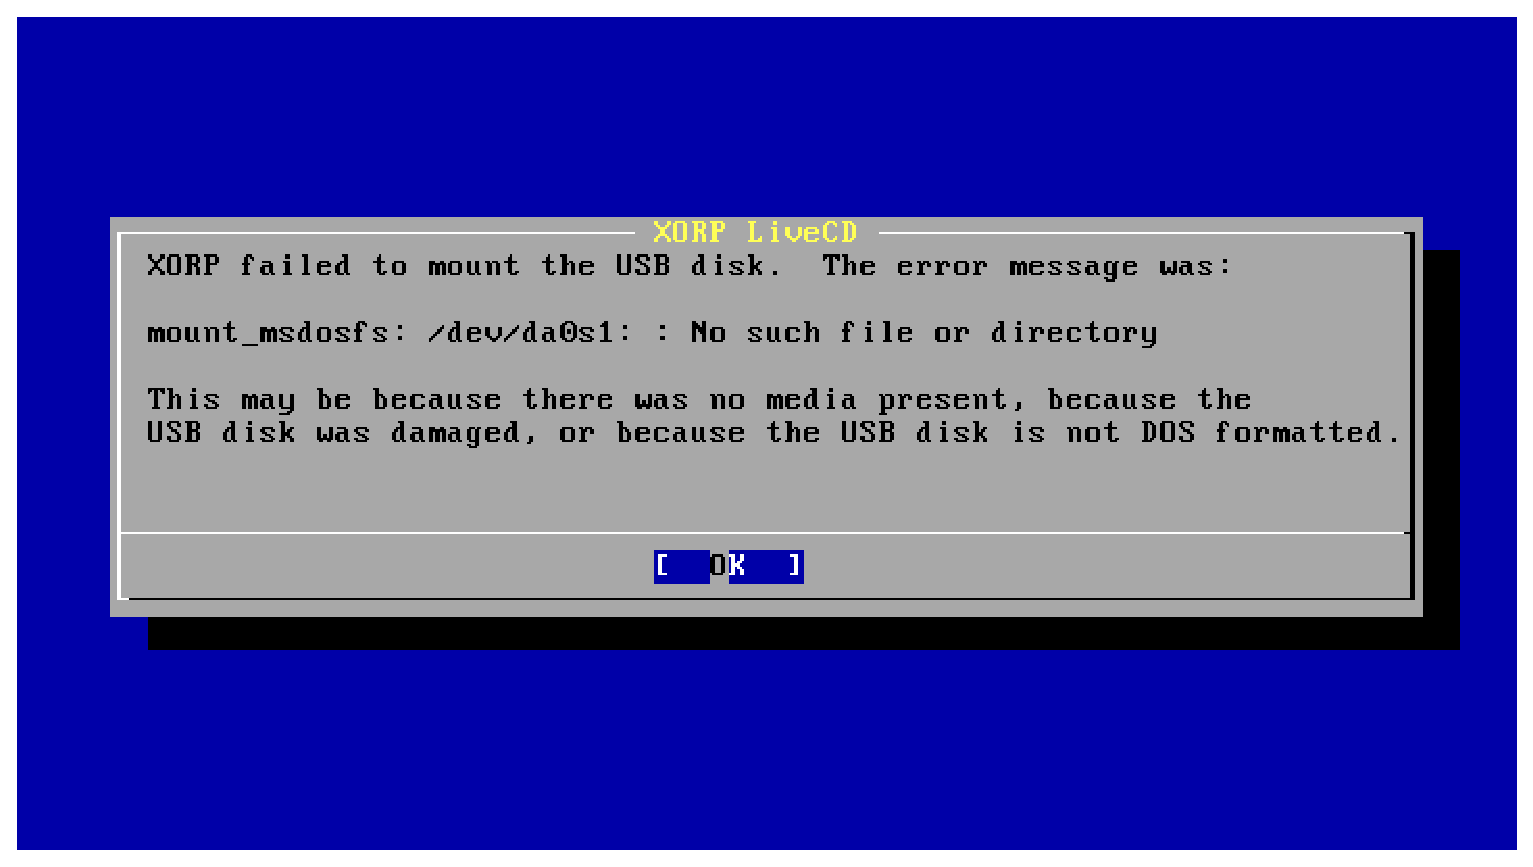
\includegraphics[width=6.0in]{figs/cd1}
    \caption{LiveCD missing configuration device warning}
    \label{fig:livecd:cd1}
  \end{center}
\end{figure}

Hit enter, and you'll be given the choices shown in
Figure~\ref{fig:livecd:cd2}.

\begin{figure}[h]
  \begin{center}
    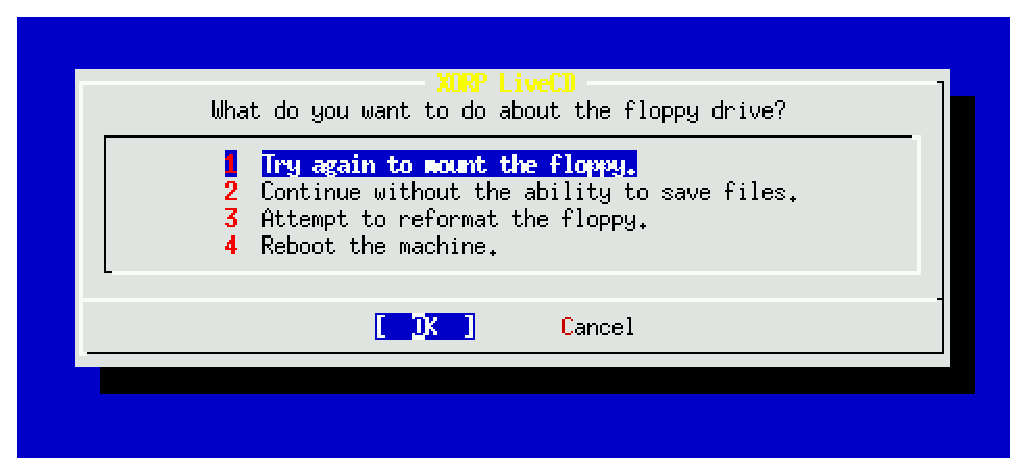
\includegraphics[width=6.0in]{figs/cd2}
    \caption{LiveCD configuration device menu}
    \label{fig:livecd:cd2}
  \end{center}
\end{figure}


Use the cursor keys to move up and down to choose an option, and hit enter.

If no USB disk is connected, you can add one now, and select 1.

If your USB disk is not DOS formatted, you can reformat it (erasing all the data
on it) by selecting 3.

If you don't have a USB disk to hand, you can continue by selecting 2,
but you won't be able to preserve any configuration changes you make
later.

If you now have a writable, DOS formatted USB device connected,
hit Enter, and you will be prompted to enter the root password for the
FreeBSD system.  This will allow you to login to the machine as the
superuser to diagnose any problems, or to see how XORP works behind
the scenes.

Next you will be prompted to enter the password for the "xorp" user
account.  On a normal XORP router, you might have many user accounts
for the different router administrators, but on the Live CD we just
create one user called "xorp".  Please do enter a reasonable password,
as this user will be able to login over the network using the ssh
secure shell and this password.

Finally you will be prompted as to which network interfaces you wish
XORP to manage.  These interfaces will show up in the default XORP
configuration file, ready to have IP addresses assigned.  The menu
looks like the one shown in Figure~\ref{fig:livecd:cd4}.

\begin{figure}[h]
  \begin{center}
    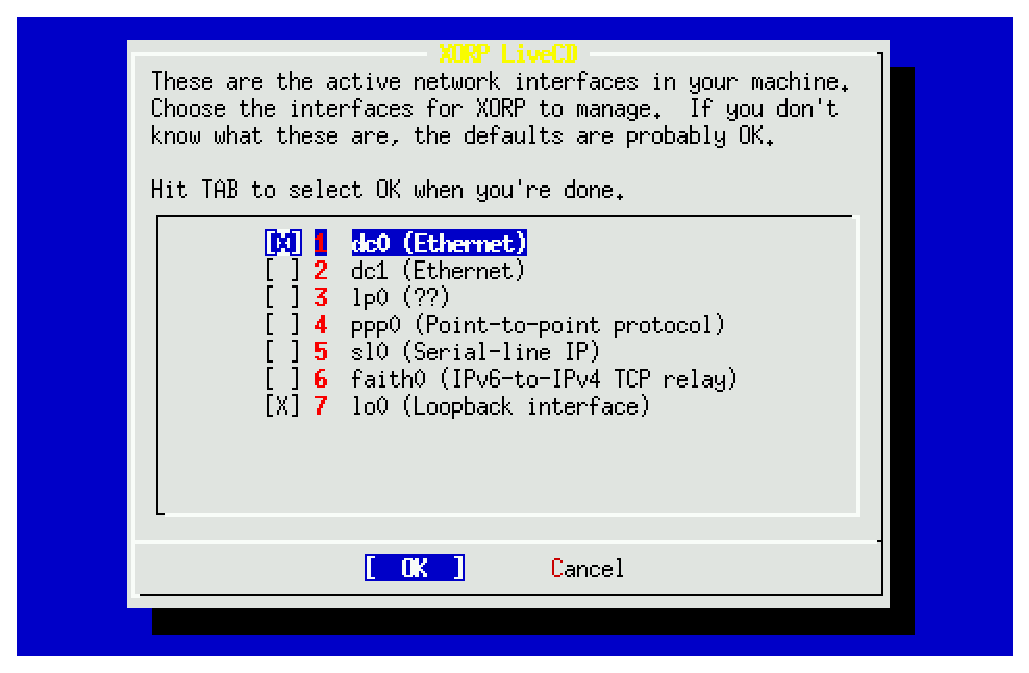
\includegraphics[width=6.0in]{figs/cd4}
    \caption{LiveCD network interfaces menu}
    \label{fig:livecd:cd4}
  \end{center}
\end{figure}

Typically you will only want XORP to manage Ethernet interfaces and
the loopback interface from the Live CD at this stage, because currently
XORP has no built-in support for dial-up links.  Move up and down using the
cursor keys, and hit space to select or unselect an option (an "X"
implies the option is selected).  When you are finished, hit Tab, to
select the "OK" button, and hit Enter.

That's it.  XORP will now finish booting.

Once XORP has finished booting, you will be presented with a login
prompt, and you can login to XORP as the "xorp" user with the password
you have chosen, and interact with the XORP command line interface to
complete the configuration, assign IP addresses, etc.

\section{Saving Config}

The location of the router configuration file used by XORP can be set
using command line parameters, so different XORP systems might choose
to use a different location for this file.  On the Live CD, the
configuration file is stored in {\stt /etc/local/xorp.conf}.

If you change the router configuration using the XORP shell, and want
to save it, you need to enter the following in configuration mode:

\vspace{0.1in}
\noindent\framebox[\textwidth][l]{\scriptsize
\begin{minipage}{6in}
\begin{alltt}
\begin{tabbing}
xxxxxxxxxxxxxxxxxx\=\kill
user@hostname\# \textbf{save /etc/local/xorp.conf}
\end{tabbing}
\end{alltt}
\end{minipage}
}
\vspace{0.1in}

If you save to any other location, the file will not be loaded automatically the next time XORP reboots.

If you want to preserve the configuration on a USB disk, use the following
command in the XORP shell's operational mode:

\vspace{0.1in}
\noindent\framebox[\textwidth][l]{\scriptsize
\begin{minipage}{6in}
\begin{alltt}
\begin{tabbing}
xxxxxxxxxxxxxxxxxx\=\kill
user@hostname> \textbf{usb save}
\end{tabbing}
\end{alltt}
\end{minipage}
}
\vspace{0.1in}


\section{Interface Naming}

If you're used to Linux, you may be surprised that FreeBSD names it's
Ethernet interfaces with names like {\stt fxp0}, {\stt fxp1},
{\stt dc0} and {\stt xl3}, rather than {\stt eth0}, {\stt eth1}, etc.
The advantage is that you can tell exactly what the device driver is
that's being used, and that if you know you have one Intel 10/100 and one
DEC Tulip in the machine, you know they'll be called {\stt fxp0} and
{\stt dc0}, no matter which PCI slot they're in.  The disadvantage is
that it's more confusing for beginners who don't want to know this detail.

Some people get religious about such things.  We don't - this just
reflects the underlying operating system's naming convention.  If you
ran XORP on Linux, you'd see {\stt eth0}, etc.


%%%%%%%%%%%%%%%%%%%%%%%%%%%%%%%%%%%%%%%%%%%%%%%%%%%%%%%%%%%%%%%%%%%%%%%
%     BIBLIOGRAPHY
%%%%%%%%%%%%%%%%%%%%%%%%%%%%%%%%%%%%%%%%%%%%%%%%%%%%%%%%%%%%%%%%%%%%%%%
\bibliography{../tex/xorp}
\bibliographystyle{plain}

%%%%%%%%%%%%%%%%%%%%%%%%%%%%%%%%%%%%%%%%%%%%%%%%%%%%%%%%%%%%%%%%%%%%%%%
\end{document}
